\pagenumbering{arabic}
%\documentclass[slides]{beamer}
\documentclass[mathserif, 8pt]{beamer}
\usepackage[framesassubsections]{beamerprosper}
\setbeamercovered{transparent}
%\documentclass[slides,hyperref={pdfpagelabels=false}]{beamer}
%\documentclass[handout,gray]{beamer}
\usepackage[T1]{fontenc}
\usepackage[utf8]{inputenc}
\usepackage{textcomp}
\usepackage{algorithm}
\usepackage{algorithmic}
\usepackage{color}
\usepackage{verbatim}
\usepackage{amsbsy}
\usepackage{multirow}
\usepackage{multicol}
\usepackage{booktabs} % Make some nice tables
\usepackage{ae,aecompl}

%%%%%%%%%%%% COULEURS %%%%%%%%%%%%%%%%%%%%%%%%%%%

\mode<presentation>
{
  \definecolor{beamerstructure}{RGB}{43,79,112}
  \definecolor{sidebackground}{RGB}{230,242,250}
  \definecolor{CTCC}{RGB}{133,188,228}
  \color{beamerstructure}
  \usetheme{default}
  \usepackage{courier}
  \beamertemplateballitem
\setbeamertemplate{navigation symbols}{}
%\setbeamertemplate{sidebar left}{\thispdfpagelabel{\insertframenumber}}
%\setbeamertemplate{footline}{\quad\insertframenumber}
%\usecolortheme{CTCC}
}
\usebackgroundtemplate{
\includegraphics[width=1.02\paperwidth]{../templets/ctcc_general.jpg}}

\title{\\\vspace{1cm}
Linear scaling Coulomb interaction with Multiwavelets}
%\subtitle{\textcolor{magenta}{My subtitle (if applicable)}}
\author{Stig Rune Jensen}
\institute[CTCC]{\\[-6mm]stig.r.jensen@uit.no\\[6mm]UiT The Arctic University of Norway\\[6mm]

\includegraphics[height=1.5cm]{../templets/uio.pdf}\hspace{1cm} 

\includegraphics[height=1.5cm]{../templets/sff.pdf}\hspace{1cm}

\includegraphics[height=1.5cm]{../templets/uit.pdf}}
\date{Paris, July 4th 2014}

\newcommand{\gb}[1]{green!#1!black}
\newcommand{\rb}[1]{red!#1!black}
\newcommand{\bb}[1]{blue!#1!black}
\newcommand{\coleq}{red!60!black}
\newcommand{\du}{\textrm{d}}

\newcommand{\mydef}{\stackrel{\text{def}}{\hbox{=}}} 
\newcommand{\Node}{\texttt{Node\ }}
\newcommand{\node}{\texttt{node\ }}
\newcommand{\nodes}{\texttt{nodes\ }}
\newcommand{\Tree}{\texttt{Tree\ }}
\newcommand{\tree}{\texttt{tree\ }}
\newcommand{\trees}{\texttt{trees\ }}

\newcommand{\red}[1]{\textcolor{red}{#1}}

\begin{document}

\footnotesize
\setlength{\unitlength}{\textwidth}

{
\usebackgroundtemplate{
\includegraphics[width=1.02\paperwidth]{../templets/ctcc_forside.jpg}}
\maketitle
}

\begin{frame}
    \frametitle{Summary}
    About the presented computer codes
    \begin{itemize}
	\item	written in C++
	\item	parallelized using OpenMP, MPI and hybrid
	\item	based on \textbf{multiresolution analysis} and the \textbf{multiwavelet basis}
    \end{itemize}
    \ \\
    \ \\
    \pause
    Features of \textbf{MultiResolution Computation Program Package (MRCPP)}
    \begin{itemize}
	\item	Multiresolution representations of functions and operators
	\item	On-the-fly adaptive multiresolution grids
	\item	Arithmetic operations and numerical integrals
	\item	\textbf{Linear scaling} application of operators
	\item	\textbf{Guaranteed accuracy}
    \end{itemize}
    \ \\
    \ \\
    \pause
    Features of \textbf{MultiResolution Grid (MRGrid)}
    \begin{itemize}
	\item	Numerical grid generator for conventional QM programs
	\item	Provide accurate and reliable numerical grids for diffuse properties
    \end{itemize}
    \ \\
    \ \\
    \pause
    Features of \textbf{MultiResolution Chemistry (MRChem)}
    \begin{itemize}
	\item	Numerical solution for the electronic structure of molecules
	\item	SCF level of theory (Hartree-Fock and DFT)
	\item	Spin-restricted and spin-unrestricted calculations
	\item	Able to attain high (guaranteed) accuracy in energies
    \end{itemize}
\end{frame}

%\begin{frame}
    %\frametitle{Outlook}
    %\begin{itemize}
	%\item   \textbf{Paper I}
	%\begin{itemize}
	    %\item   Multiwavelets
	    %\item   Function representations
	    %\item   Varying polynomial order
	%\end{itemize}
	%\ \\
	%\ \\
	%\item   \textbf{Paper II}
	%\begin{itemize}
	    %\item   Operator representation
	    %\item   Parallel implementation
	    %\item   Coulomb interaction
	%\end{itemize}
	%\ \\
	%\ \\
	%\item   \textbf{Paper III}
	%\begin{itemize}
	    %\item   Density Functional Theory
	    %\item   Integral formulation
	    %\item   Iterative algorithm
	%\end{itemize}
    %\end{itemize}
%\end{frame}

%\begin{frame}
    %\centering
    %\Large{Part I:}\\
    %\ \\
    %\ \\
    %\centering
    %\Large{Adaptive order polynomial algorithm in a\\
	    %multiwavelet representation scheme}
%\end{frame}

\begin{frame}
    \frametitle{Multiwavelets}
    \begin{columns}
    \begin{column}[b]{0.55\linewidth}
	\begin{itemize}
	    \item   \textbf{Scaling functions} are polynomials or order $\leq k$\\
		    on the unit interval
	    \item   \textbf{Dilation and translation} to refinement scale $n$
		    \begin{equation}
			\nonumber
			\phi_l^n(x) = 2^{n/2}\phi(2^nx-l)
		    \end{equation}
	    \item   At scale $n$ there are $2^n$ subintervals
	    \item   The length of each subinterval is $2^{-n}$
	    \item   \textbf{Scaling projection} at scale $N$
		    \begin{equation}
			\nonumber
			f(x) \approx f^N(x) = \sum_l s_l^N \phi_l^N(x)
		    \end{equation}
		    \ \\
		    \ \\
	    \item   For a $k$-order basis in $d$ dimensions there are\\
		    $\left(2(k+1)\right)^{nd}$ basis functions at scale $n$\\
	\end{itemize}
	\centering
	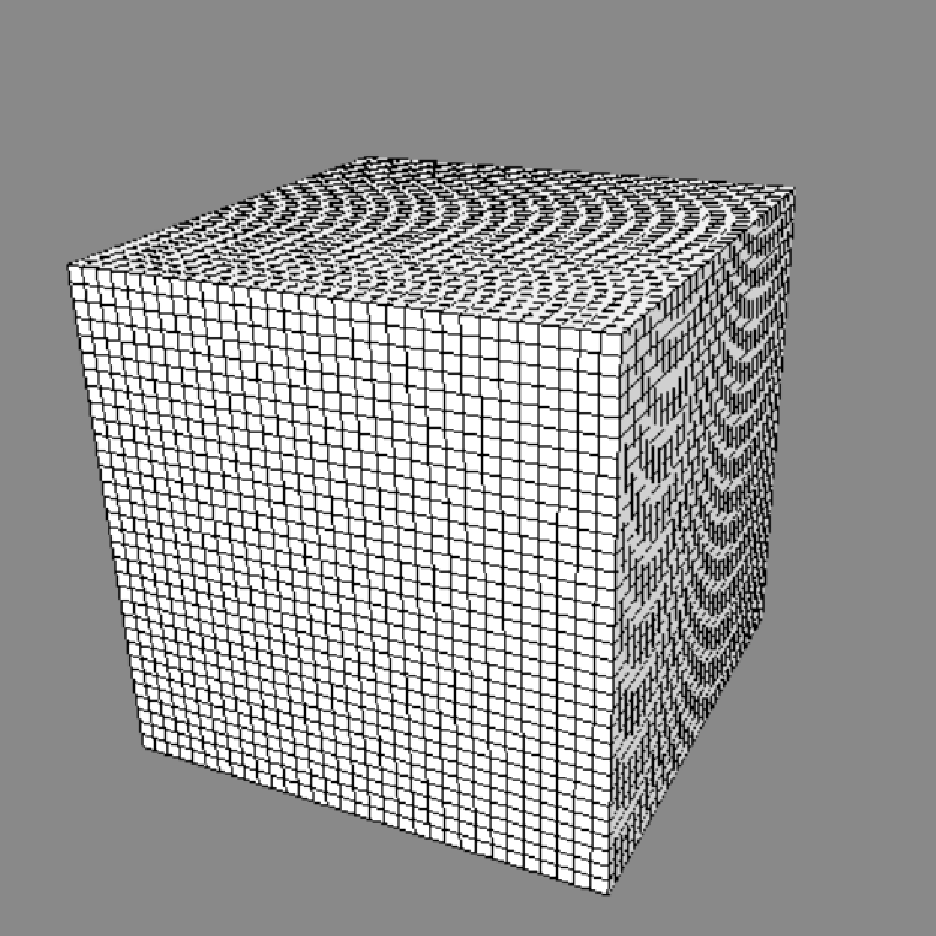
\includegraphics[scale=0.2]{figures/unifgrid.pdf}
    \end{column}
    \begin{column}[b]{0.45\linewidth}
	\centering
	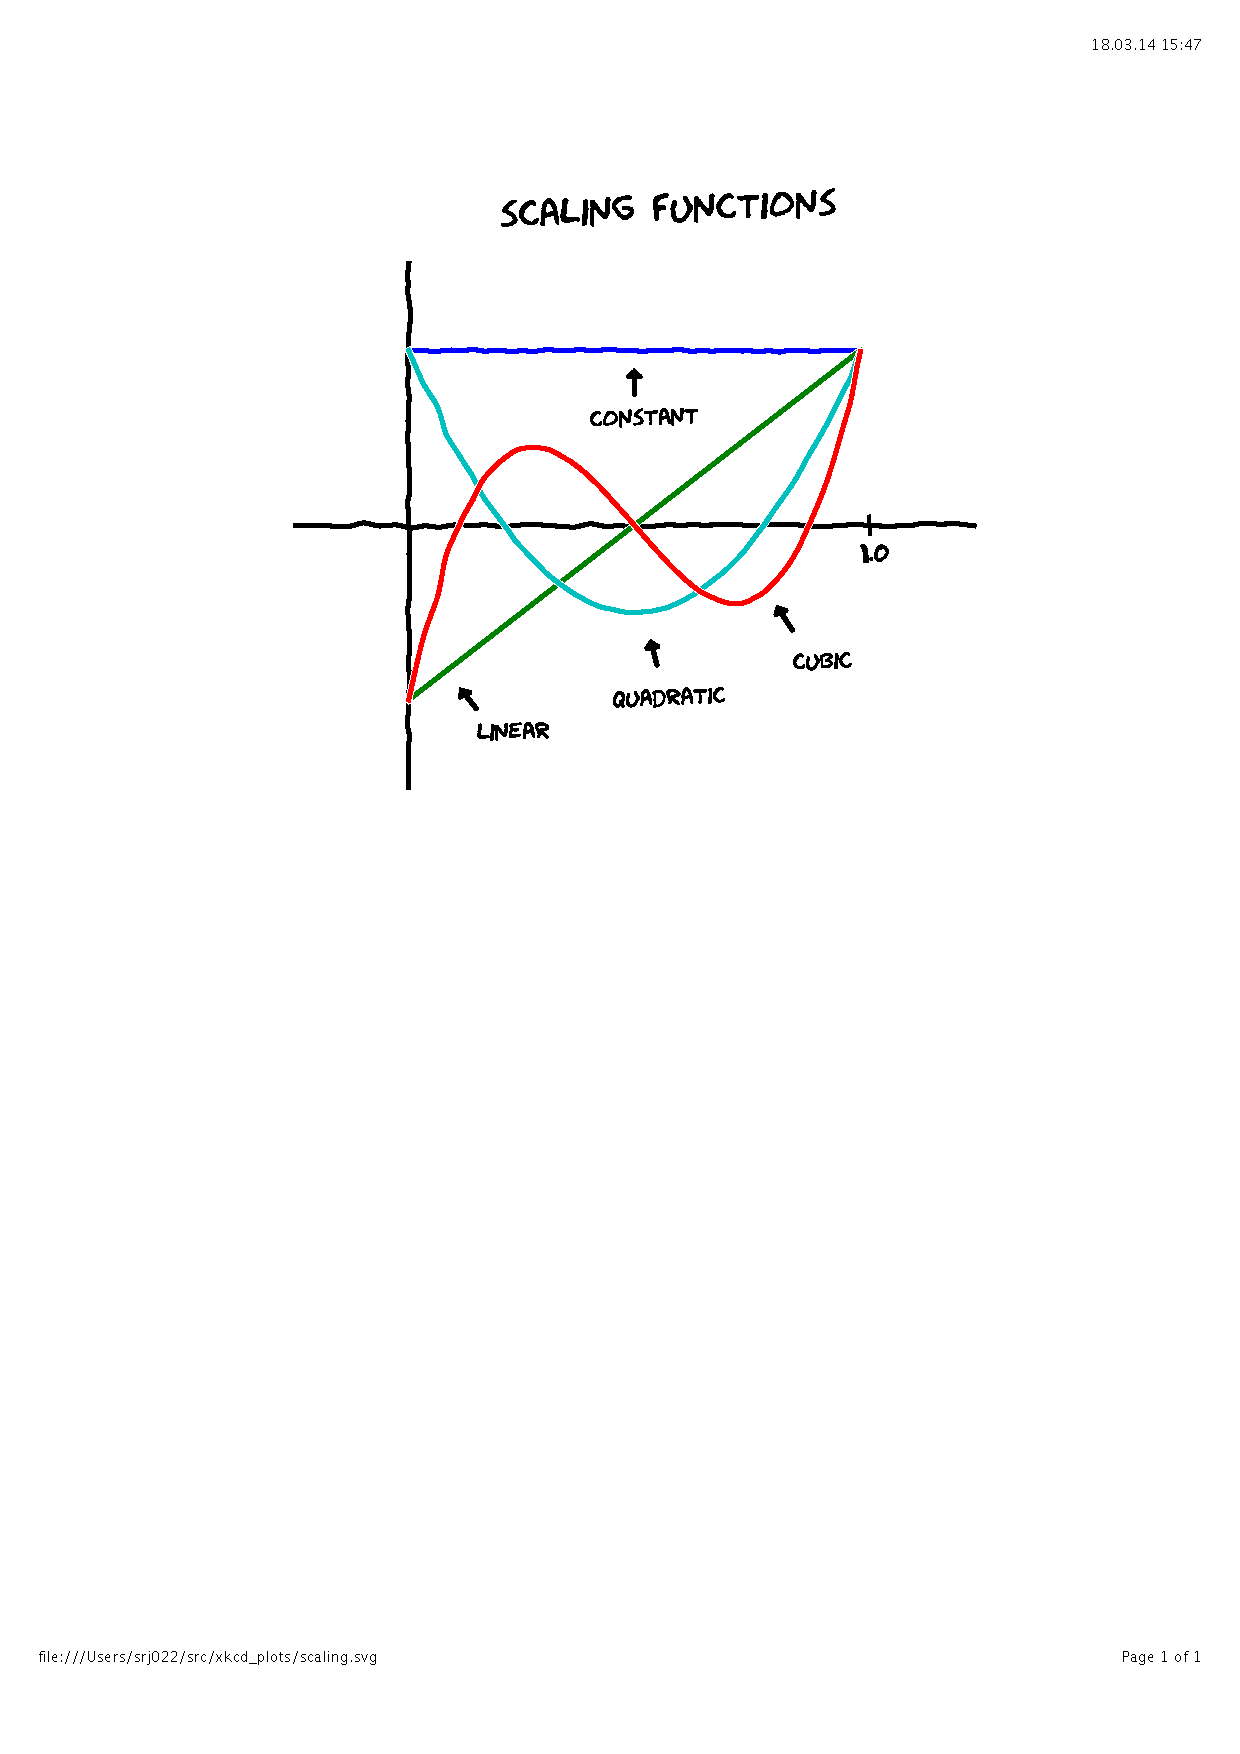
\includegraphics[scale=0.3, clip, viewport = 150 450 450 750]{figures/scaling.pdf}\\
	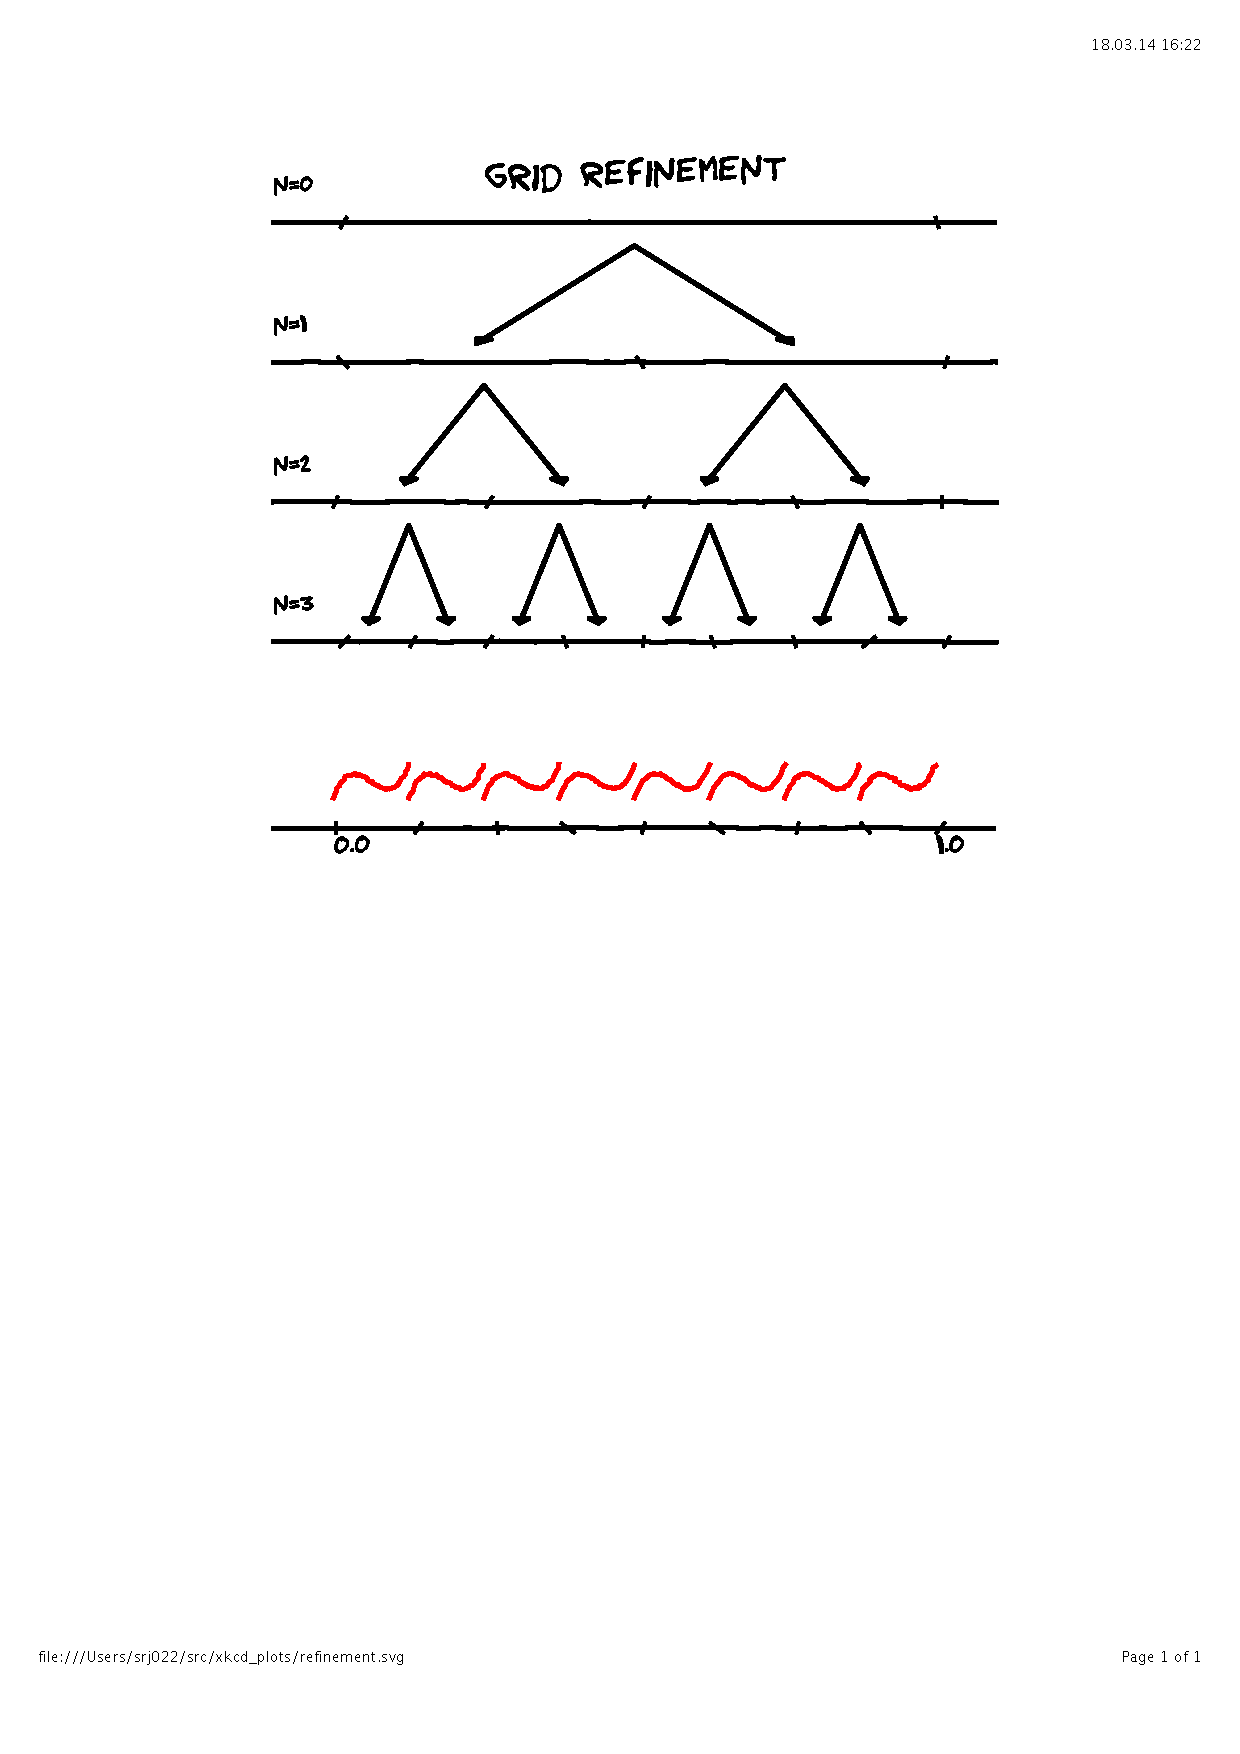
\includegraphics[scale=0.3, clip, viewport = 100 400 500 800]{figures/refinement.pdf}
    \end{column}
    \end{columns}
\end{frame}

\begin{frame}
    \frametitle{Multiwavelets}
    \centering
    \only<1>{\ \ \ 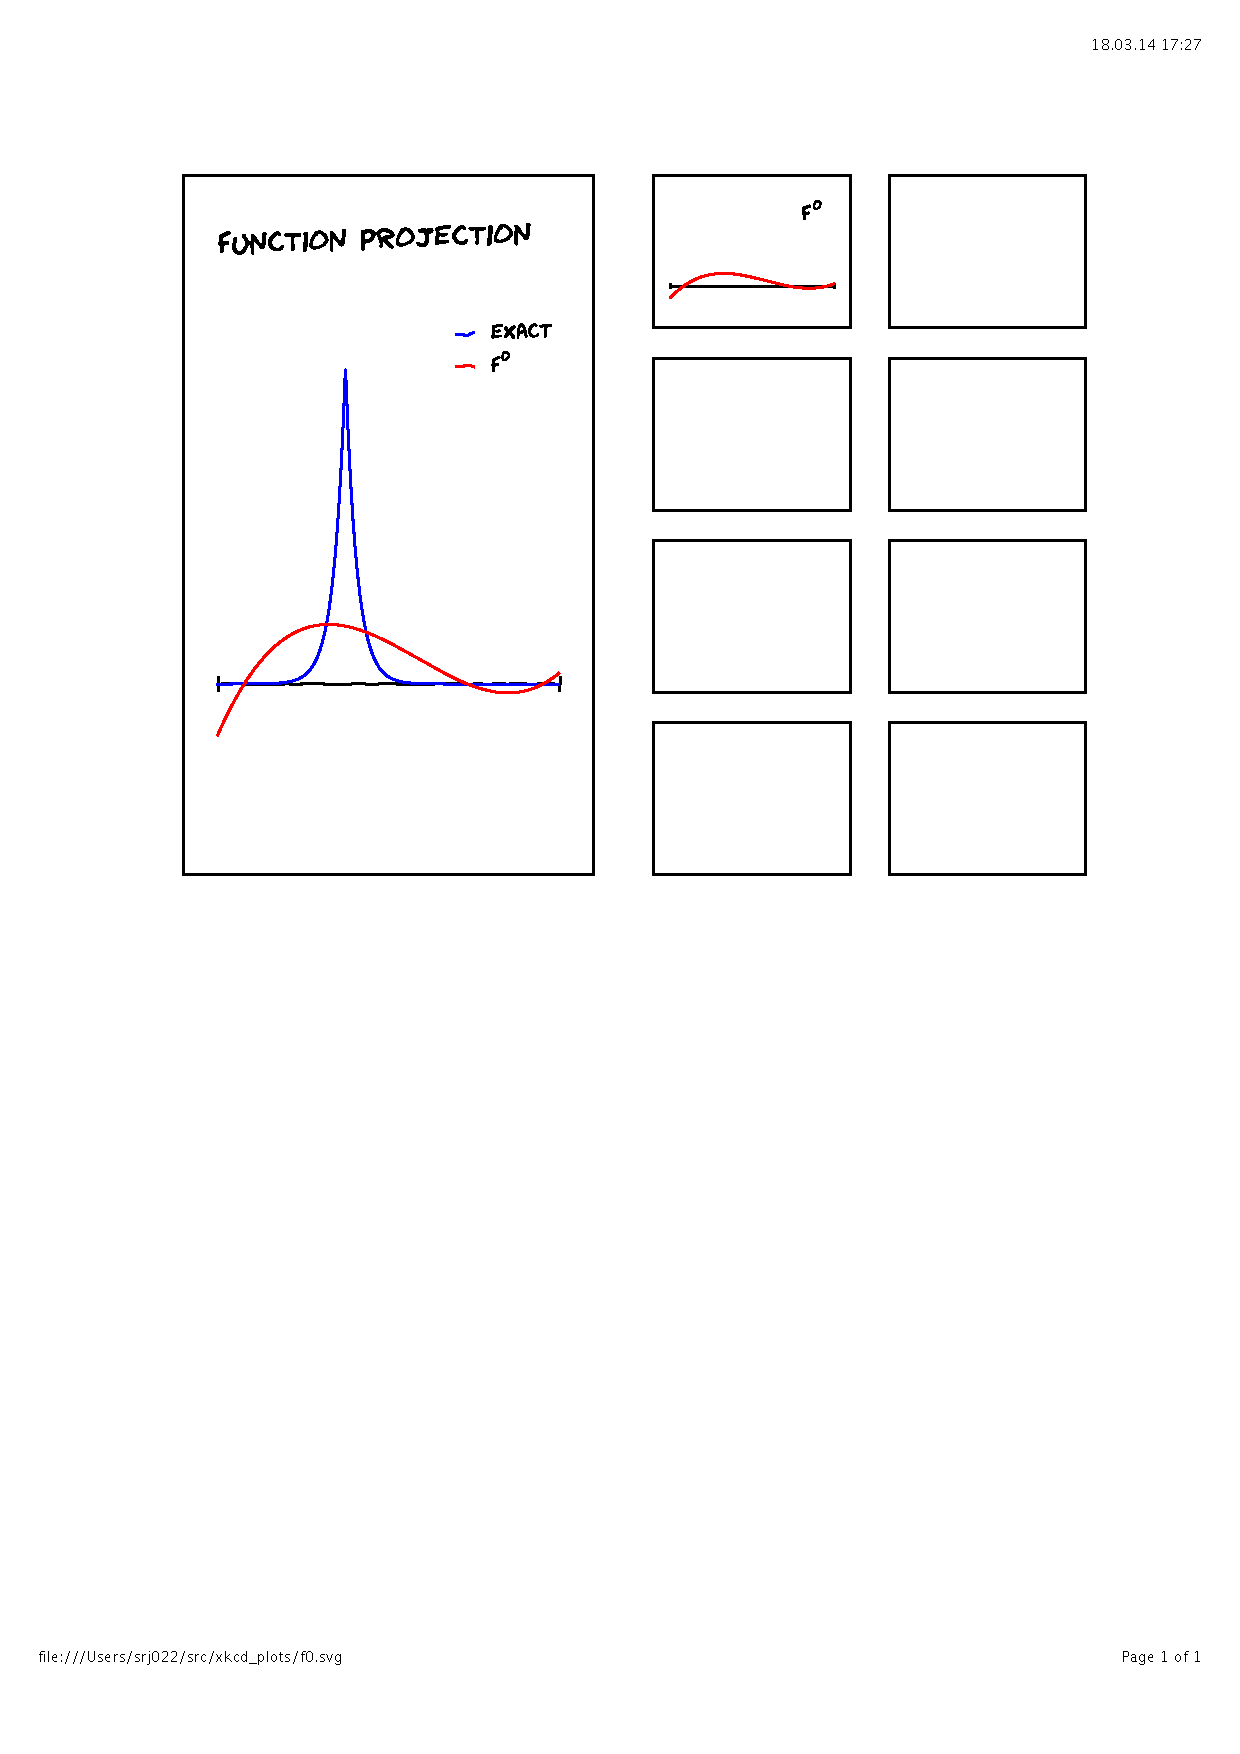
\includegraphics[clip, viewport=50 100 600 800, scale=0.5]{figures/f0.pdf}}
    \only<2>{\ \ 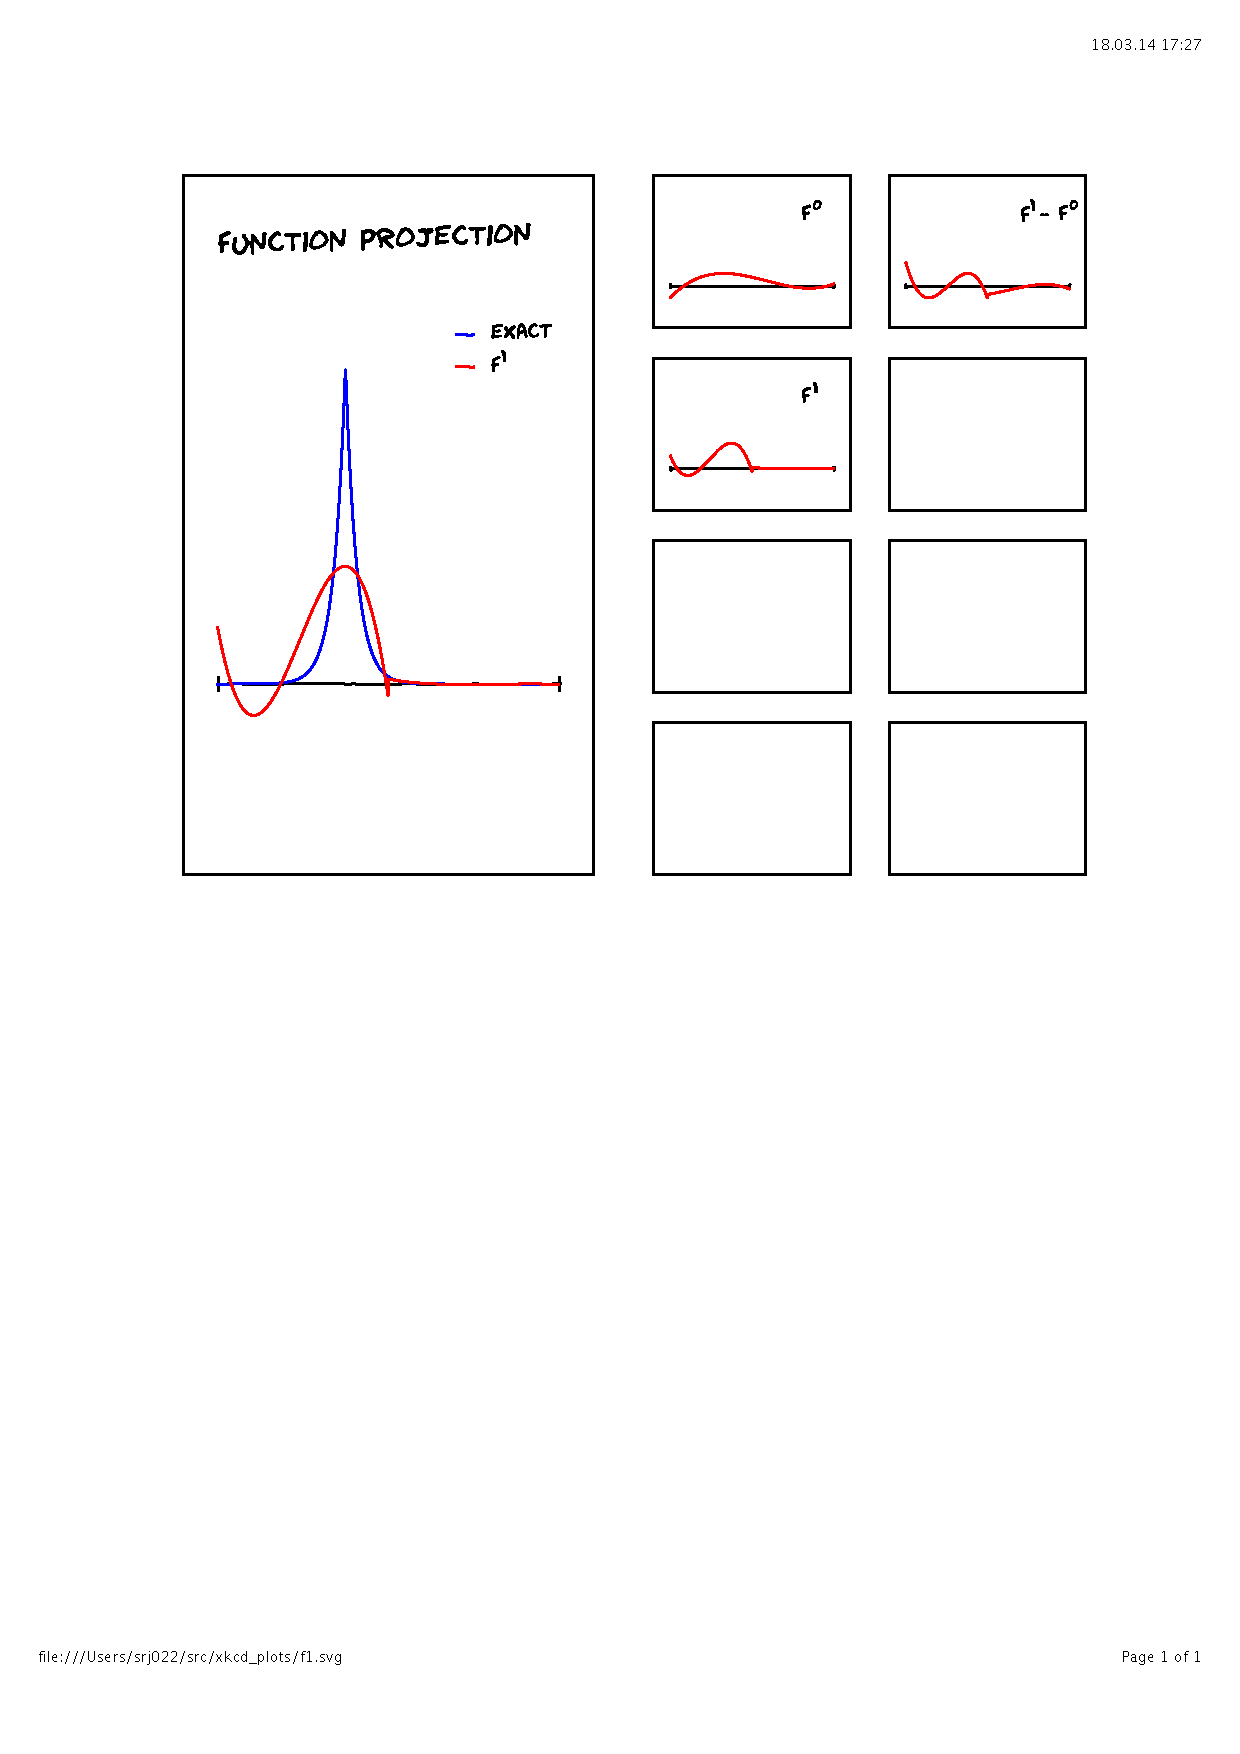
\includegraphics[clip, viewport=50 100 600 800, scale=0.5]{figures/f1.pdf}}
    \only<3>{\ 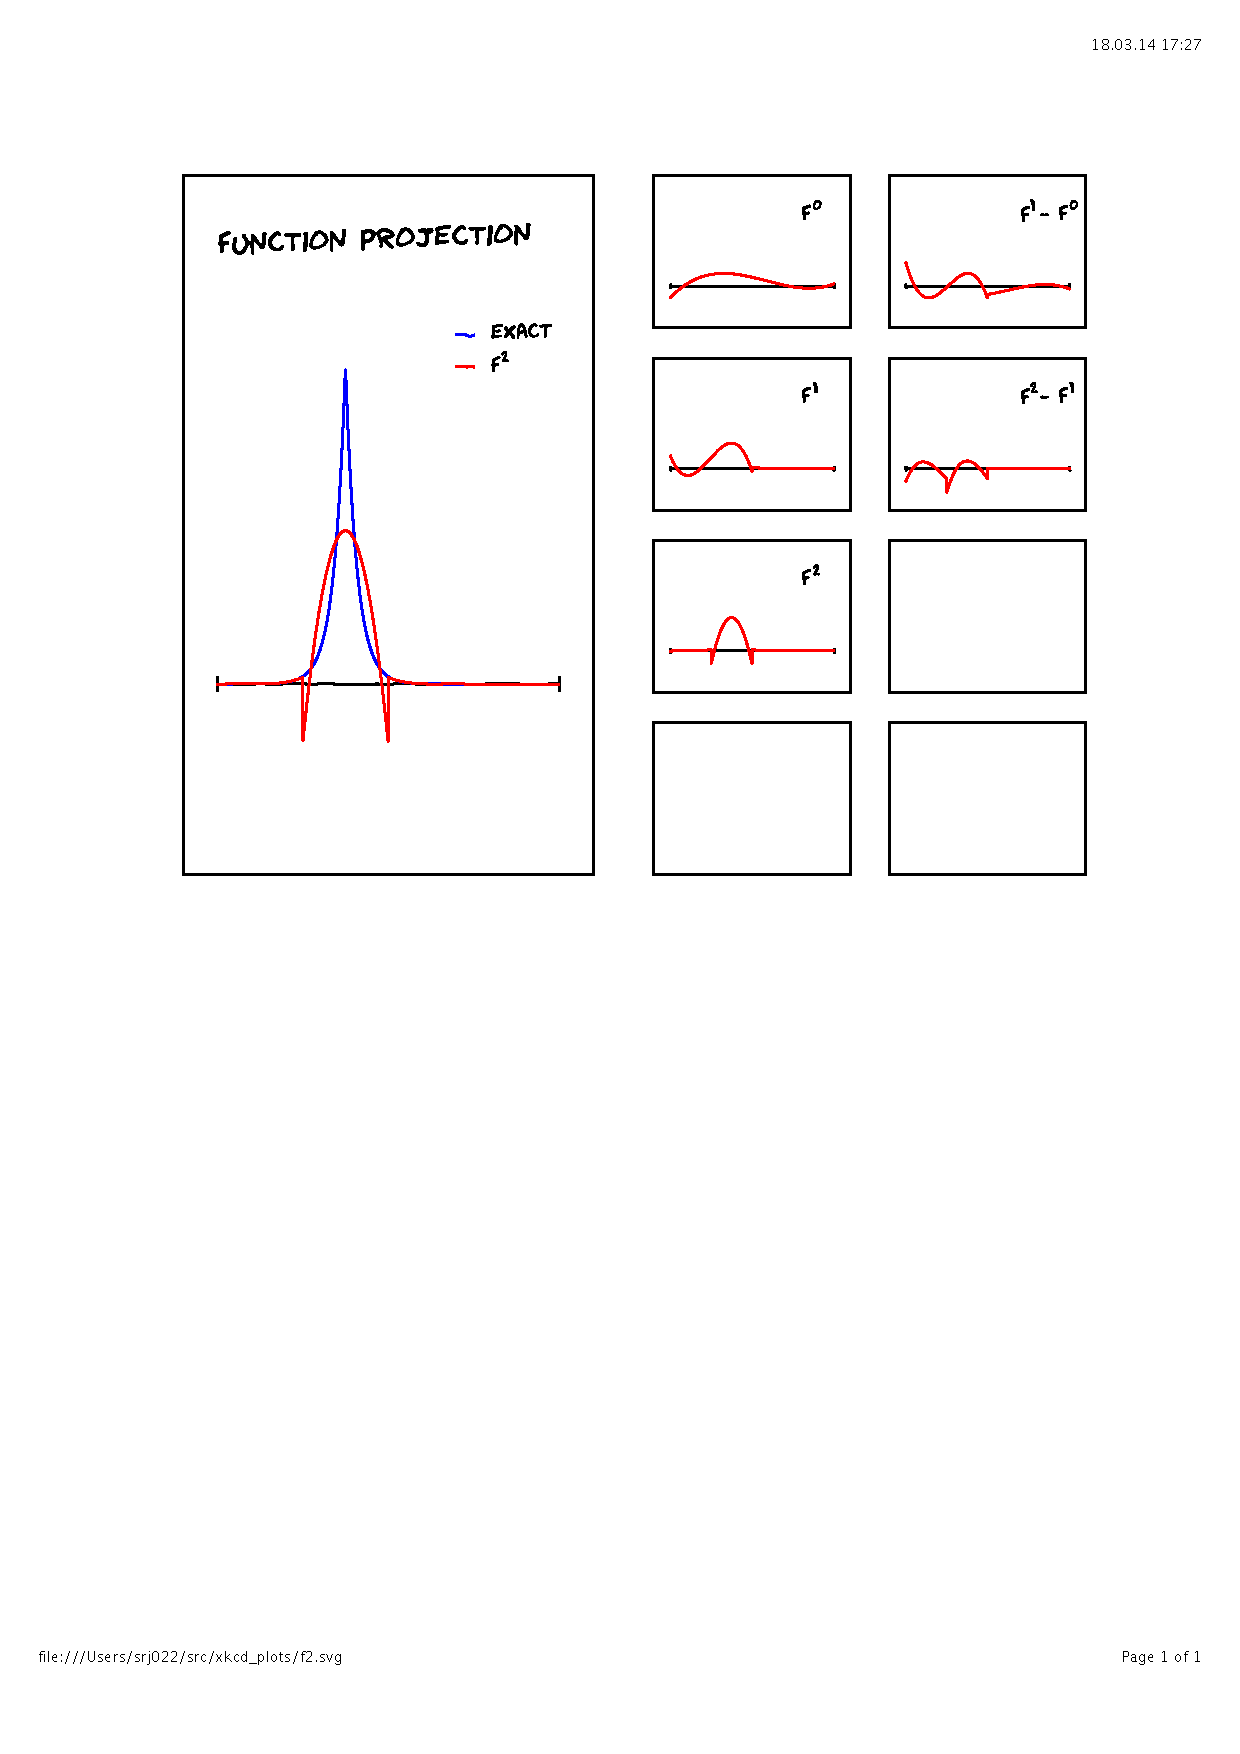
\includegraphics[clip, viewport=50 100 600 800, scale=0.5]{figures/f2.pdf}}
    \only<4>{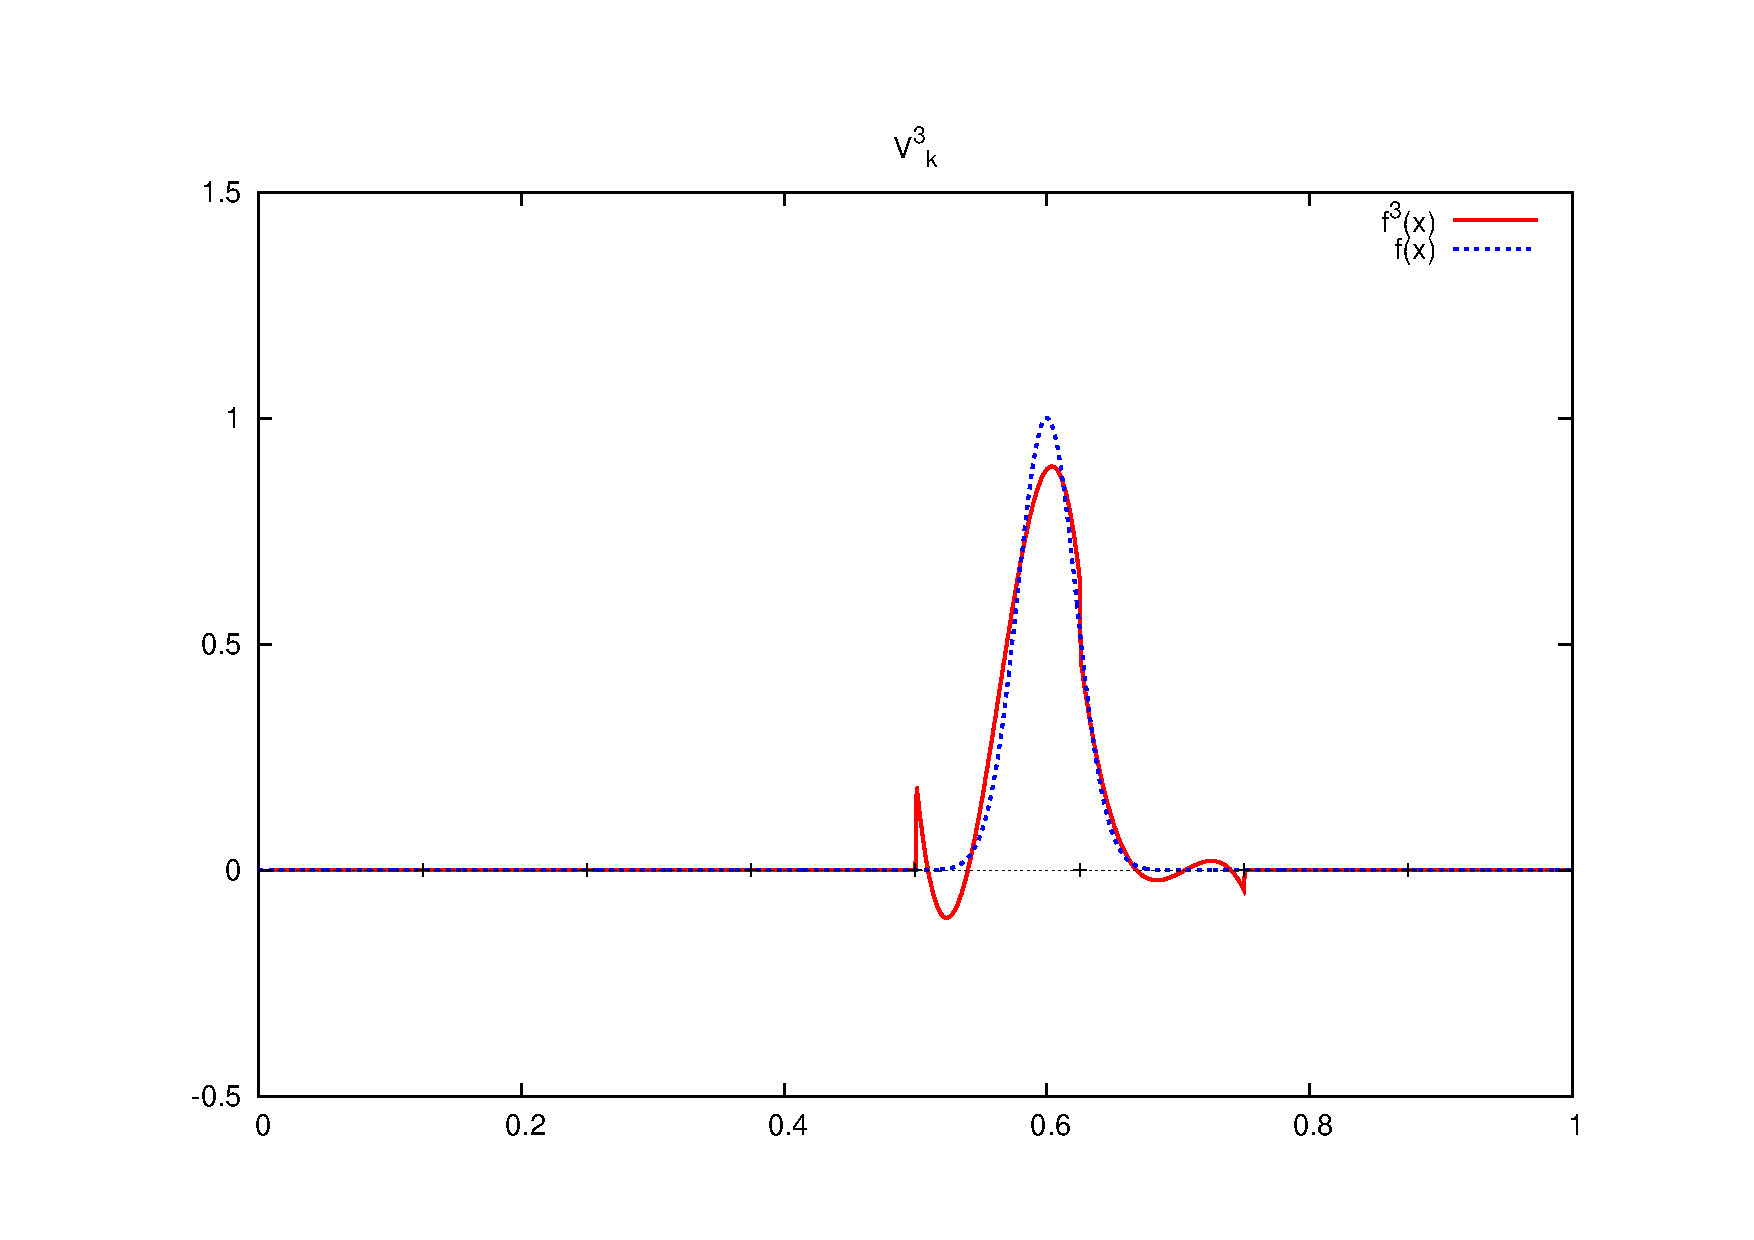
\includegraphics[clip, viewport=50 100 600 800, scale=0.5]{figures/f3.pdf}}
    \only<5>{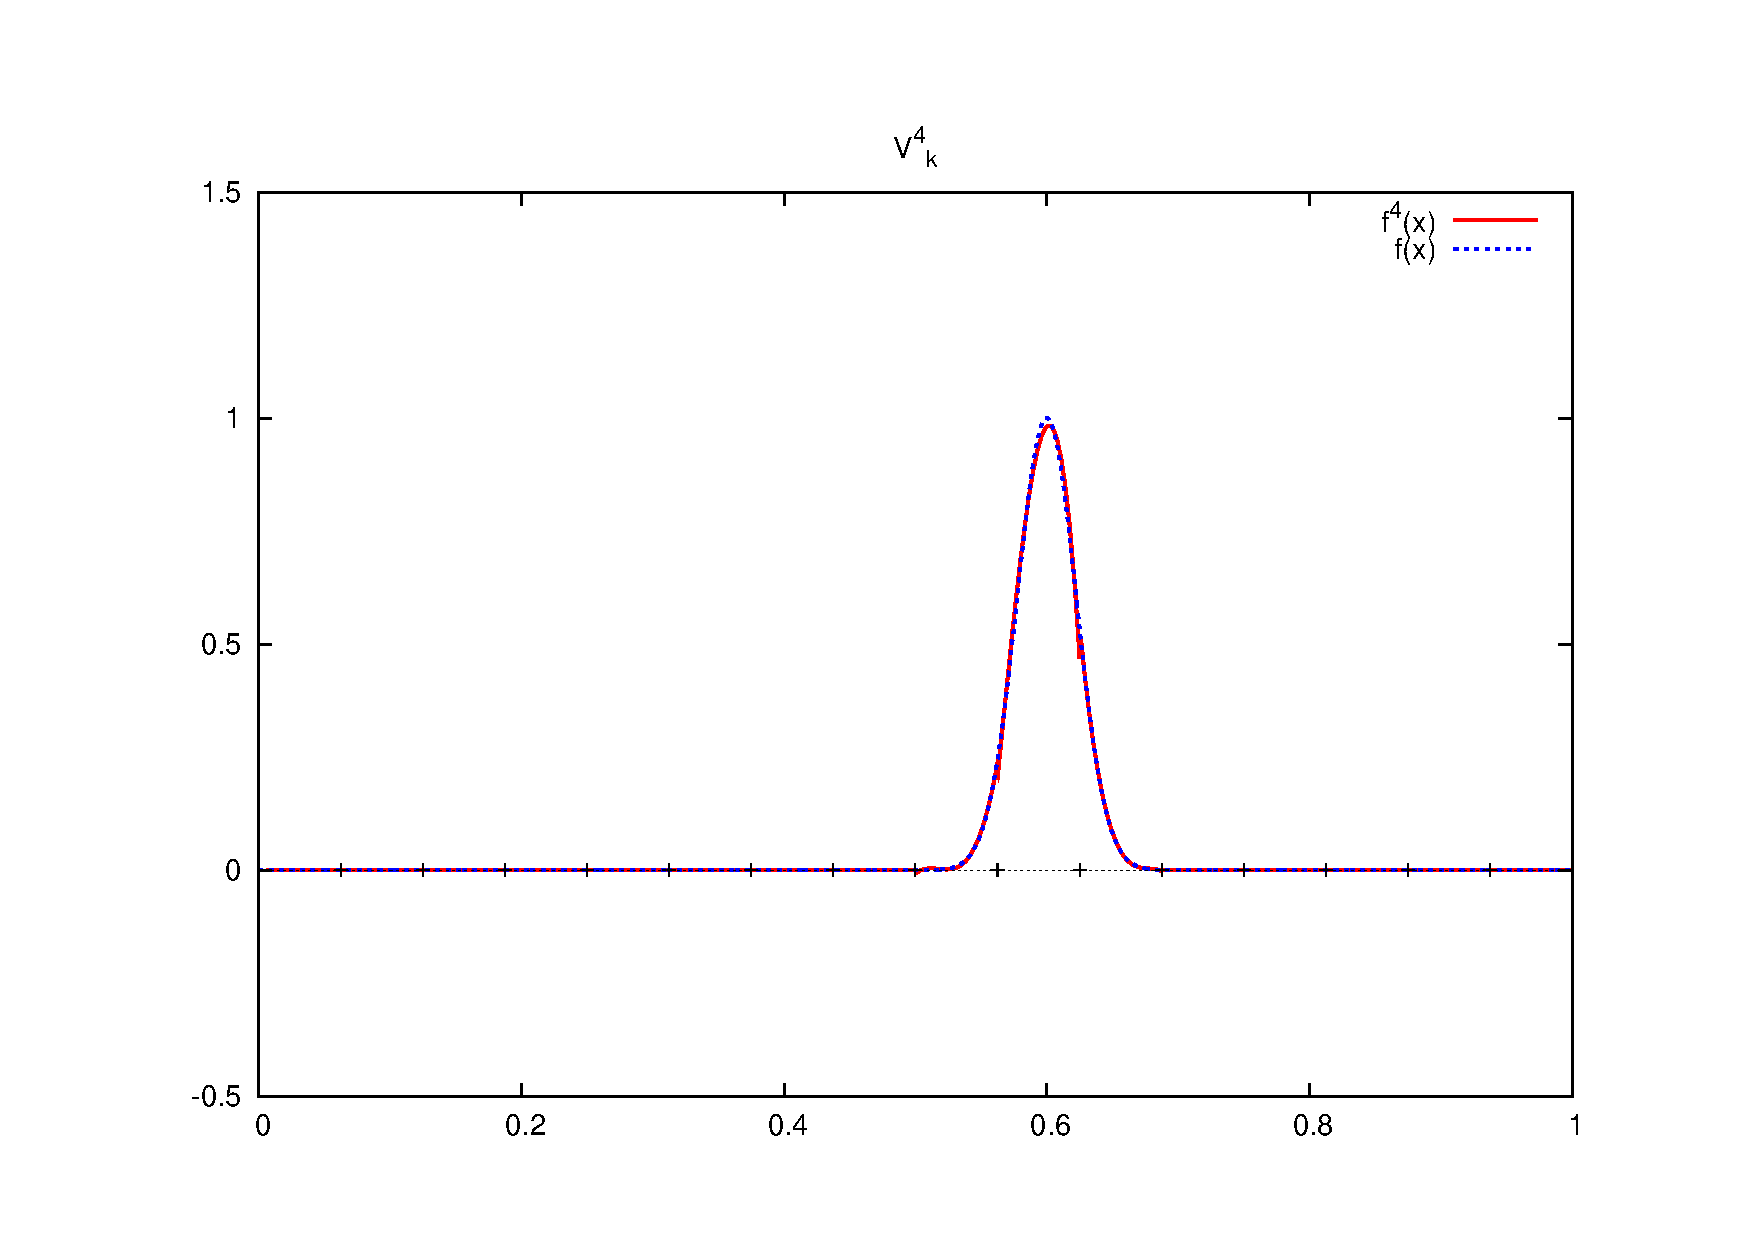
\includegraphics[clip, viewport=50 100 600 800, scale=0.5]{figures/f4.pdf}}
\end{frame}

\begin{frame}
    \frametitle{Multiwavelets}
    \begin{columns}
    \begin{column}[b]{0.55\linewidth}
	\begin{itemize}
	    \item   \textbf{Wavelet functions} are piecewise polynomials
	    \item   \textbf{Wavelet projection} at scale $n$
		    \begin{equation}
			\nonumber
			df^n(x) = f^{n+1}(x) - f^{n}(x)
		    \end{equation}
		    \ \\
	    \item   Alternative \textbf{multiresolution} representation
		    \begin{equation}
			\nonumber
			f^N(x) = f^{0}(x) + \sum_{n=0}^{N-1} df^{n}(x)
		    \end{equation}
	    \item   Allows for \textbf{adaptive refinement} by local thresholding
		    \begin{equation}
			\nonumber
			\|df_l^n\| < \frac{\epsilon}{2^{n/2}}\|f\|
		    \end{equation}
	    \item   Representations with \textbf{guaranteed precision} $\epsilon$
	\end{itemize}
	\ \\
	\ \\
    \end{column}
    \begin{column}[b]{0.45\linewidth}
	\centering
	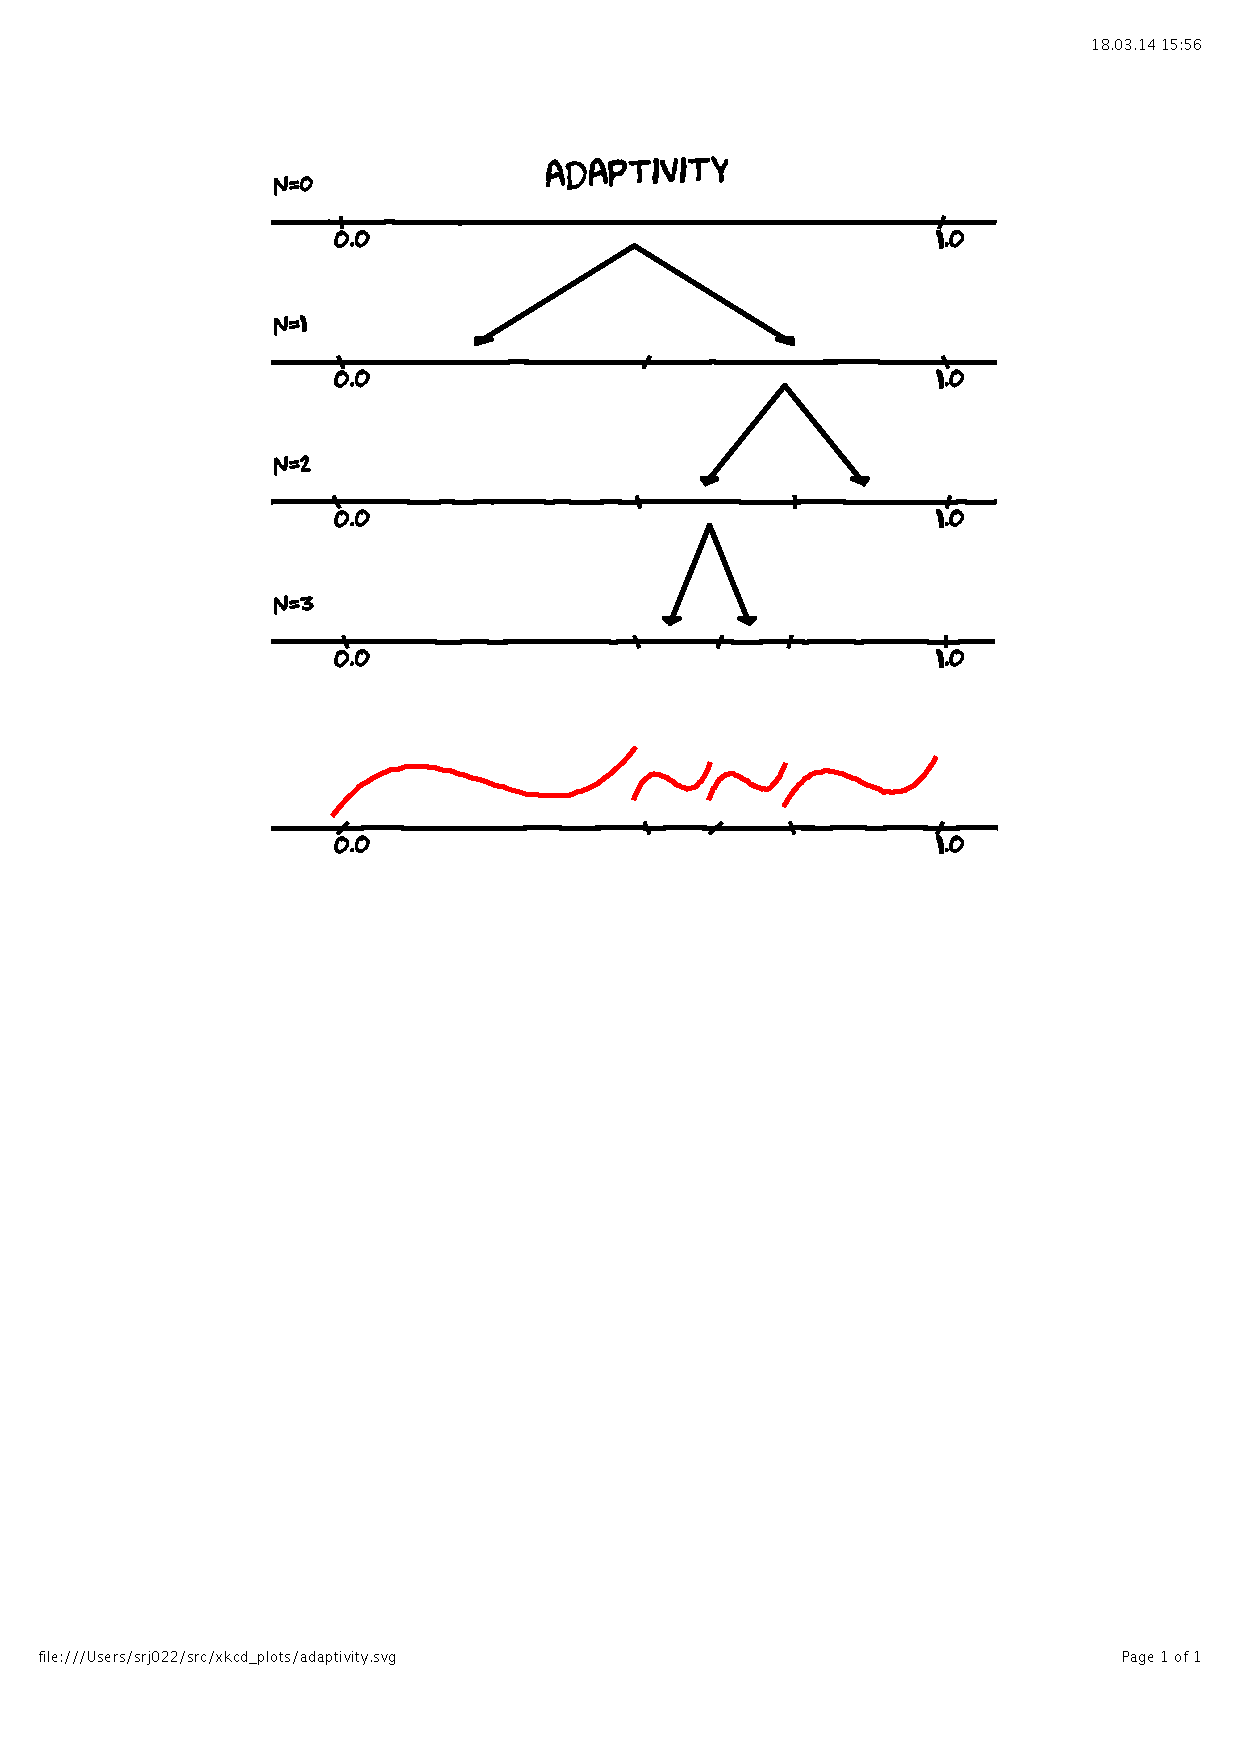
\includegraphics[scale=0.3, clip, viewport = 100 400 500 800]{figures/adaptivity.pdf}
    \end{column}
    \end{columns}
    \ \\
    \centering
    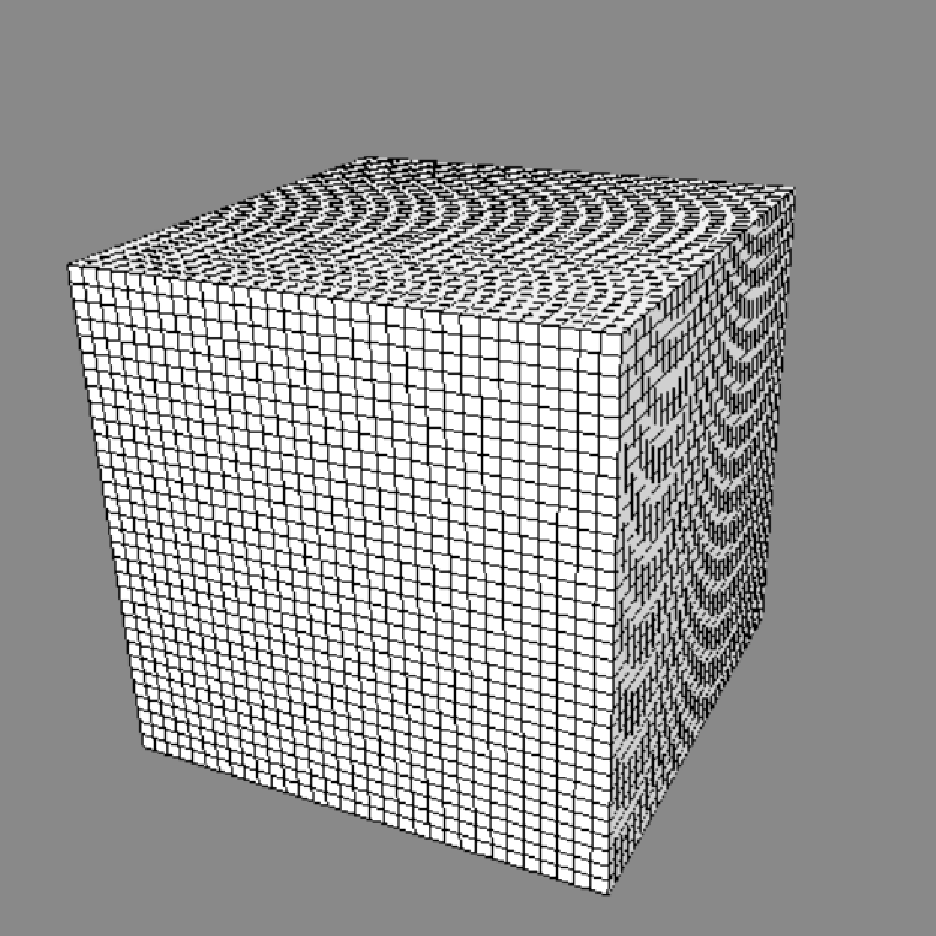
\includegraphics[scale=0.2]{figures/unifgrid.pdf}
    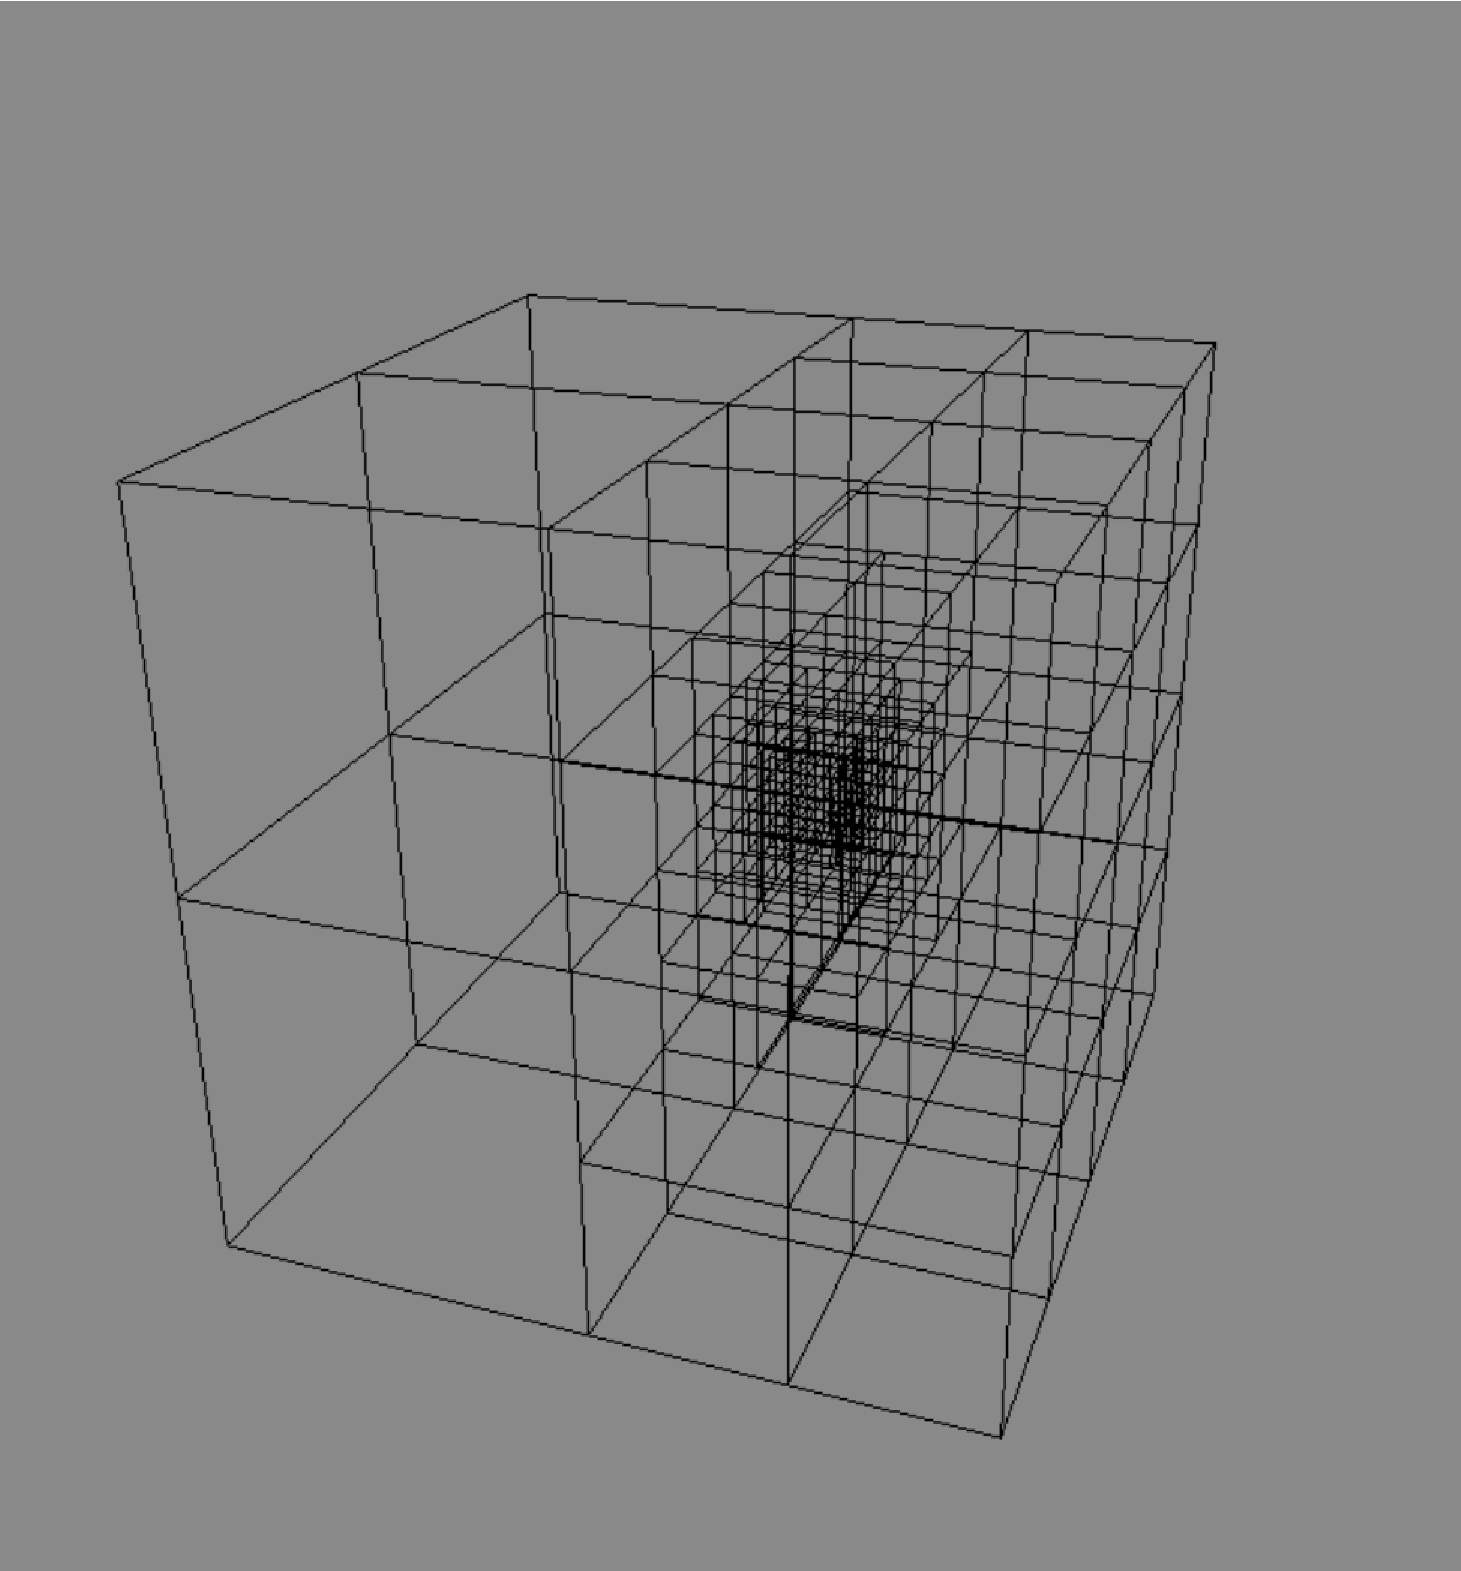
\includegraphics[scale=0.1192]{figures/adapgrid.pdf}
\end{frame}


%\begin{frame}
    %\frametitle{Decreasing order polynomial basis}
    %\begin{columns}
    %\begin{column}[b]{0.7\linewidth}
	%\begin{itemize}
	    %\item   Multi-dimensional functions require many expansion coefficients\\
		    %\ \\
	    %\item   Try to reduce the memory footprint by varying the polynomial order\\
		    %\ \\
	    %\item   Specifically decreasing the order $k$ with increasing scale $n$
	%\end{itemize}
	%\ \\
	%\ \\
	%\ \\
    %\end{column}
    %\begin{column}[b]{0.3\linewidth}
    %\centering
    %\begin{figure}
	%\setlength{\unitlength}{.5mm}
	%\begin{picture}(93,46)
	    %\put( 0,10){\vector(1,0){60}} %n- axis
	    %\put(61,10){$n$}
	    %\put(10,4){\vector(0,1){37}} %k-axis
	    %\put(10,43){$k$}
	    %\put(40,38){$k(n)$}
	    %\put(-5,30){$k_{\max}$}
	    %\put(-5,15){$k_{\min}$}
	    %\put(25,5){$n_0$}
	    %\put(40,5){$n_1$}
	    %\put(10,30){\line(1,0){15}}
	    %\put(25,30){\line(1,-1){15}}
	    %\put(40,15){\line(1,0){15}}
	    %\multiput(40,10)(0,0.1){5}{\line(0,1){2}} 
	    %\multiput(25,10)(0,4){5}{\line(0,1){2}}
	    %\multiput(10,15)(6,0){5}{\line(1,0){2}}
	%\end{picture}
    %\end{figure}
    %\end{column}
    %\end{columns}
    %\ \\
    %\centering
    %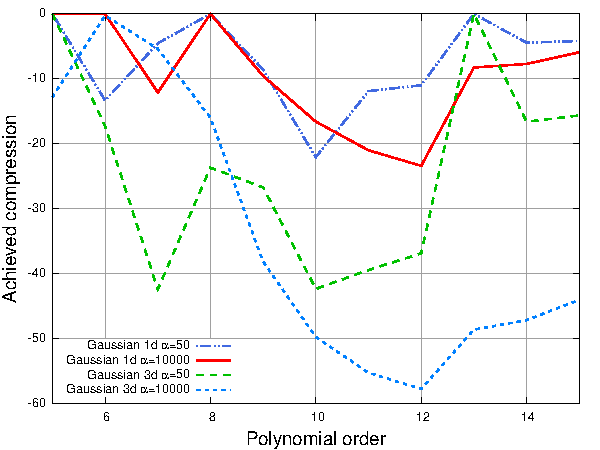
\includegraphics[scale=0.6]{figures/decrease.pdf}
%\end{frame}
%
%\begin{frame}
    %\centering
    %\Large{Part II:}\\
    %\ \\
    %\ \\
    %\centering
    %\Large{Linear scaling Coulomb interaction in the multiwavelet basis,\\
	%a parallel implementation}
%\end{frame}
%
\begin{frame}
    \frametitle{Operator representation}
    \begin{columns}
    \begin{column}[b]{0.5\linewidth}
    \begin{itemize}
	\item	The multiwavelet basis is well suited for\\ \textbf{integral convolution operators}
	    \begin{equation}
		\nonumber
		g(\boldsymbol{r}) = \left[T f\right](\boldsymbol{r}) = 
		    \int K(\boldsymbol{r} - \boldsymbol{r'})f(\boldsymbol{r'}) d\boldsymbol{r'}
	    \end{equation}
	    \ \\
	    \ \\
	\item \textbf{Scaling projection} of operator at scale $n$
	    \begin{equation}
		\nonumber
		T \approx T^n
	    \end{equation}
	\item \textbf{Wavelet projections} obtained by the difference
	    \begin{equation}
		\nonumber
		T^{n+1} - T^n = A^n + B^n + C^n
	    \end{equation}
	\item \textbf{Multiresolution operator} obtained by recursion
	    \begin{equation}
		\nonumber
		T^N = T^0 + \sum_{n=0}^{N-1} \left[A^n + B^n + C^n\right]
	    \end{equation}
	\item Scaling operator $T$ is \textbf{dense}
	\item Wavelet operators $A$, $B$ and $C$ are \textbf{sparse} 
    \end{itemize}
    \end{column}
    \begin{column}[b]{0.5\linewidth}
    \begin{center}
    \only<2>{\ \ \ 
\includegraphics[scale=0.6, clip, viewport = 240 280 450 480]{figures/matrix/matrix_1.pdf}}
    \only<3>{\ \ 
\includegraphics[scale=0.6, clip, viewport = 240 280 450 480]{figures/matrix/matrix_2.pdf}}
    \only<4>{\ 
\includegraphics[scale=0.6, clip, viewport = 240 280 450 480]{figures/matrix/matrix_3.pdf}}
    \only<5>{
\includegraphics[scale=0.6, clip, viewport = 240 280 450 480]{figures/matrix/matrix_4.pdf}}
    \only<6>{
\includegraphics[scale=0.6, clip, viewport = 240 280 450 480]{figures/matrix/matrix_5.pdf}}
    \only<7,8>{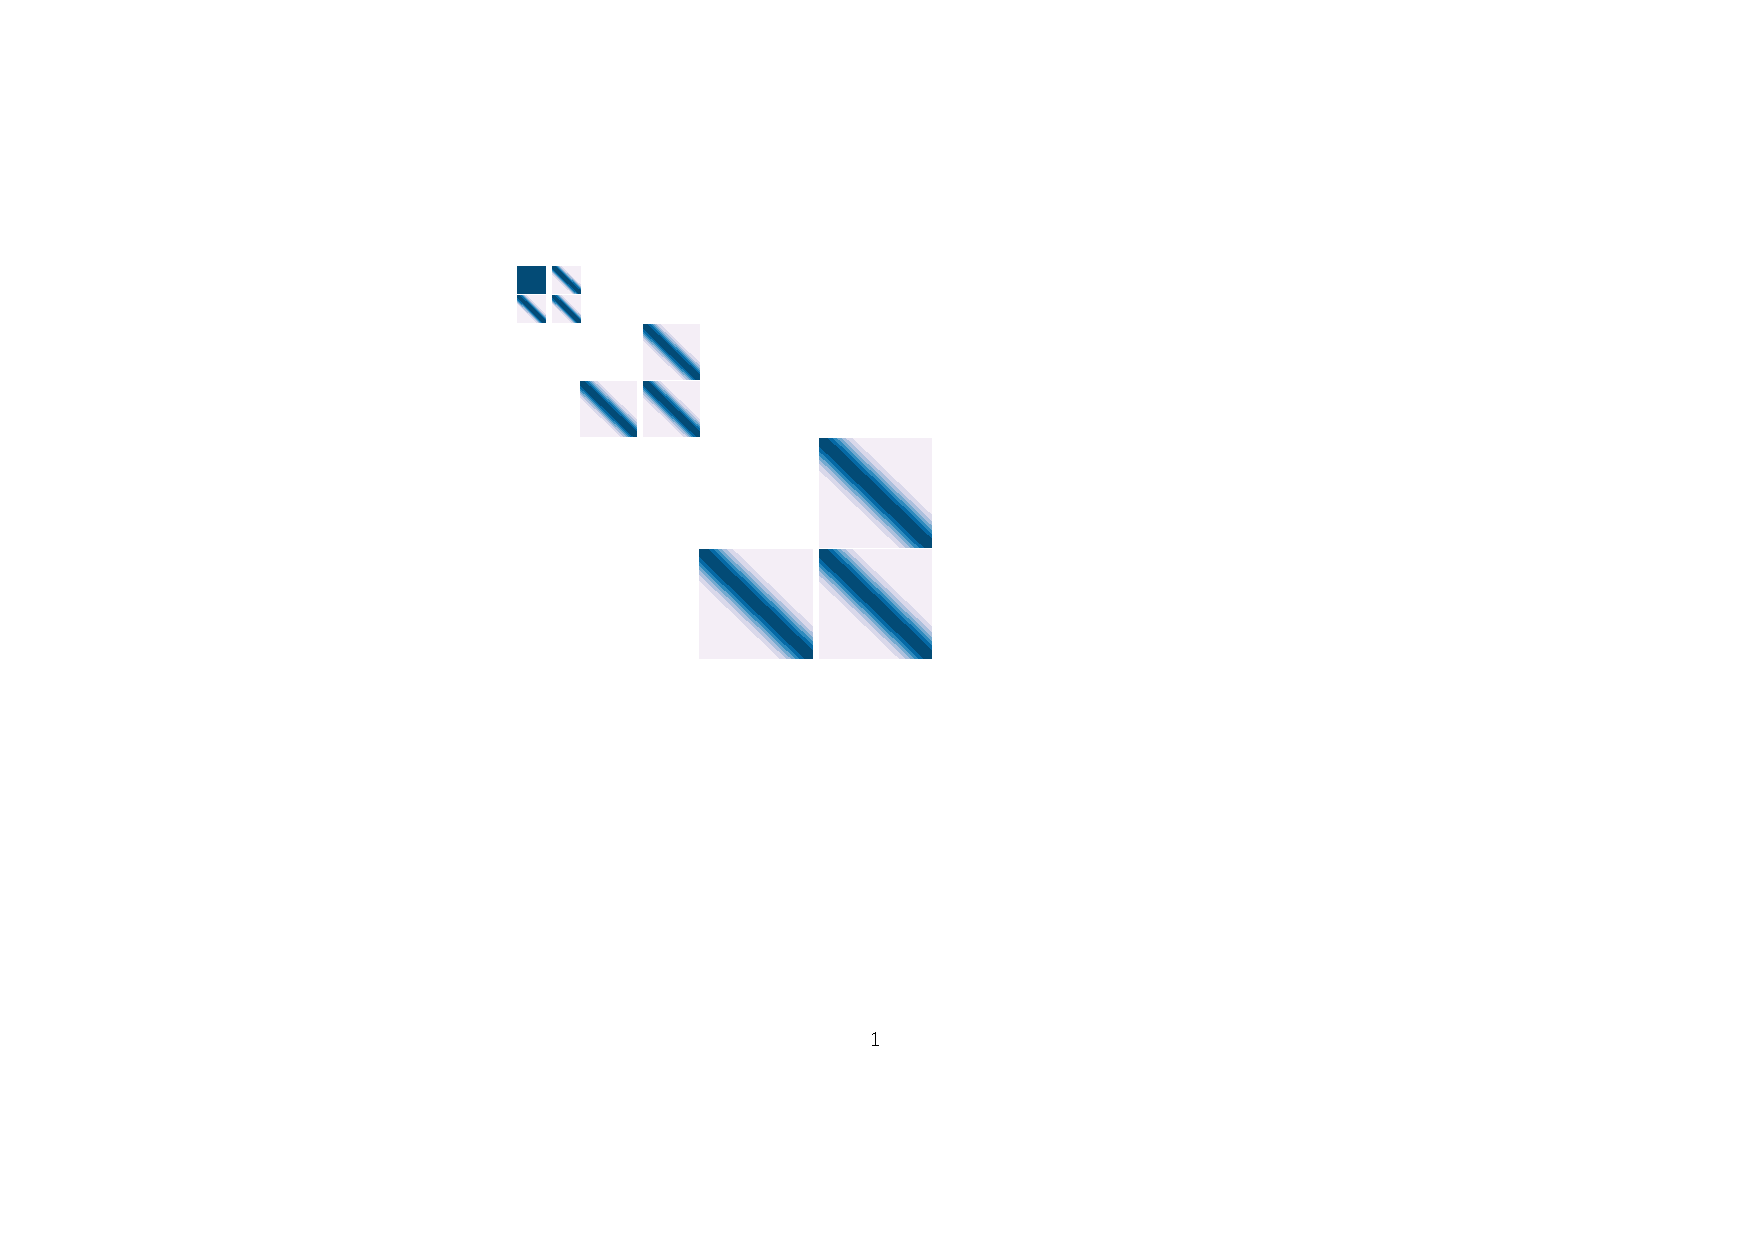
\includegraphics[scale=0.6, clip, viewport = 240 280 450 480]{figures/matrix/matrix_6.pdf}}
    \ \\
    \ \\
    \ \\
    \end{center}
    \end{column}
    \end{columns}
    \ \\
    \ \\
    \ \\
    \ \\
    \pause
    \pause
    \pause
    \pause
    \pause
    \pause
    \pause
    \begin{columns}
    \begin{column}{.30\textwidth}
    \centering
    \textbf{Poisson kernel}
    \begin{equation}
	\nonumber
	P(\boldsymbol{r}-\boldsymbol{r}') = 
	    \frac{1}{4\pi}\ \frac{1}{|\boldsymbol{r}-\boldsymbol{r}'|}
    \end{equation}
    \end{column}
    \begin{column}{.30\textwidth}
    \centering
    \textbf{Helmholtz kernel}
    \begin{equation}
	\nonumber
	H^{\mu}(\boldsymbol{r}-\boldsymbol{r}') = \frac{1}{4\pi}\ 
	    \frac{e^{-\mu |\boldsymbol{r}-\boldsymbol{r}'|}}{|\boldsymbol{r}-\boldsymbol{r}'|}
    \end{equation}
    \end{column}
    \begin{column}{.30\textwidth}
    \centering
    \textbf{Derivative kernel}
    \begin{equation}
	\nonumber
	D(x-x') = \frac{d}{dx}\delta(x-x')
    \end{equation}
    \end{column}
    \end{columns}    
\end{frame}

\begin{frame}
    \frametitle{Coulomb interaction}
    \begin{itemize}
	\item	Electrostatic potential from a \textbf{point charge} follows from Coulomb's law
		\begin{equation}
		    \nonumber
		    V(\boldsymbol{r}) = \frac{q}{4\pi\epsilon_0}
		    \frac{1}{|\boldsymbol{r}-\boldsymbol{r}'|}
		\end{equation}
		\ \\
		\ \\
		\ \\
	\item	Electrostatic potential from a \textbf{charge density} is given by the Poisson equation
		\begin{equation}
		    \nonumber
		    \nabla^2 V(\boldsymbol{r}) = -\rho(\boldsymbol{r})
		\end{equation}
		\ \\
		\ \\
		\ \\
	\item	Can be solved directly in integral form using the Poisson kernel
		\begin{equation}
		    \nonumber
		    V(\boldsymbol{r}) = 
		    \int P(\boldsymbol{r}-\boldsymbol{r'})\rho(\boldsymbol{r'}) d\boldsymbol{r'} =
		    \int\frac{\rho(\boldsymbol{r'})}{4\pi|\boldsymbol{r} - \boldsymbol{r'}|} d\boldsymbol{r'} 
		\end{equation}
		\ \\
		\ \\
		\ \\
    \end{itemize}
    \ \\
    \ \\
    \ \\
    \begin{columns}
    \begin{column}{.30\textwidth}
        \ \\
    \end{column}
    \begin{column}{.40\textwidth}
        \ \ \ \ \textbf{Numerical problems}
        \begin{itemize}
	    \item Not Cartesian separable
	    \item Singularity at short-range
	    \item Slow decay at long-range
	\end{itemize}
    \end{column}
    \begin{column}{.30\textwidth}
	\ \\
    \end{column}
    \end{columns}
\end{frame}

\begin{frame}
    \frametitle{Separation of variables using Gaussians}
    \begin{columns}
    \begin{column}{.50\textwidth}
    \begin{itemize}
	\item The Poisson kernel can be approximated as
	    \begin{equation}
		\nonumber
		P(\boldsymbol{r}) = \frac{1}{4\pi\boldsymbol{r}} \approx \sum_{i=1}^M a_i e^{-\alpha_i \boldsymbol{r}^2} 
	    \end{equation}
	\item Any accuracy can in principle be obtained
	\item Full operator is decomposed into $M$ components
	\item Each separated component is further decomposed using MRA
	\item Each operator term is applied separately
    \end{itemize}
    \ \\
    \ \\
    \ \\
    \ \\
    \ \\
    \pause
    \pause
    \pause
    \pause
    \pause
    \pause
    \pause
    \ \ \ \ \textbf{Solves problems}
    \begin{itemize}
	\item	Separates coordinates
	\item	Removes singularity
	\item	Separates length scales
    \end{itemize}
    \end{column}
    \begin{column}{.50\textwidth}
	\only<1,2,3,4,5>{\ \\}
	\only<1>{\ \ \ \ \ \ \ 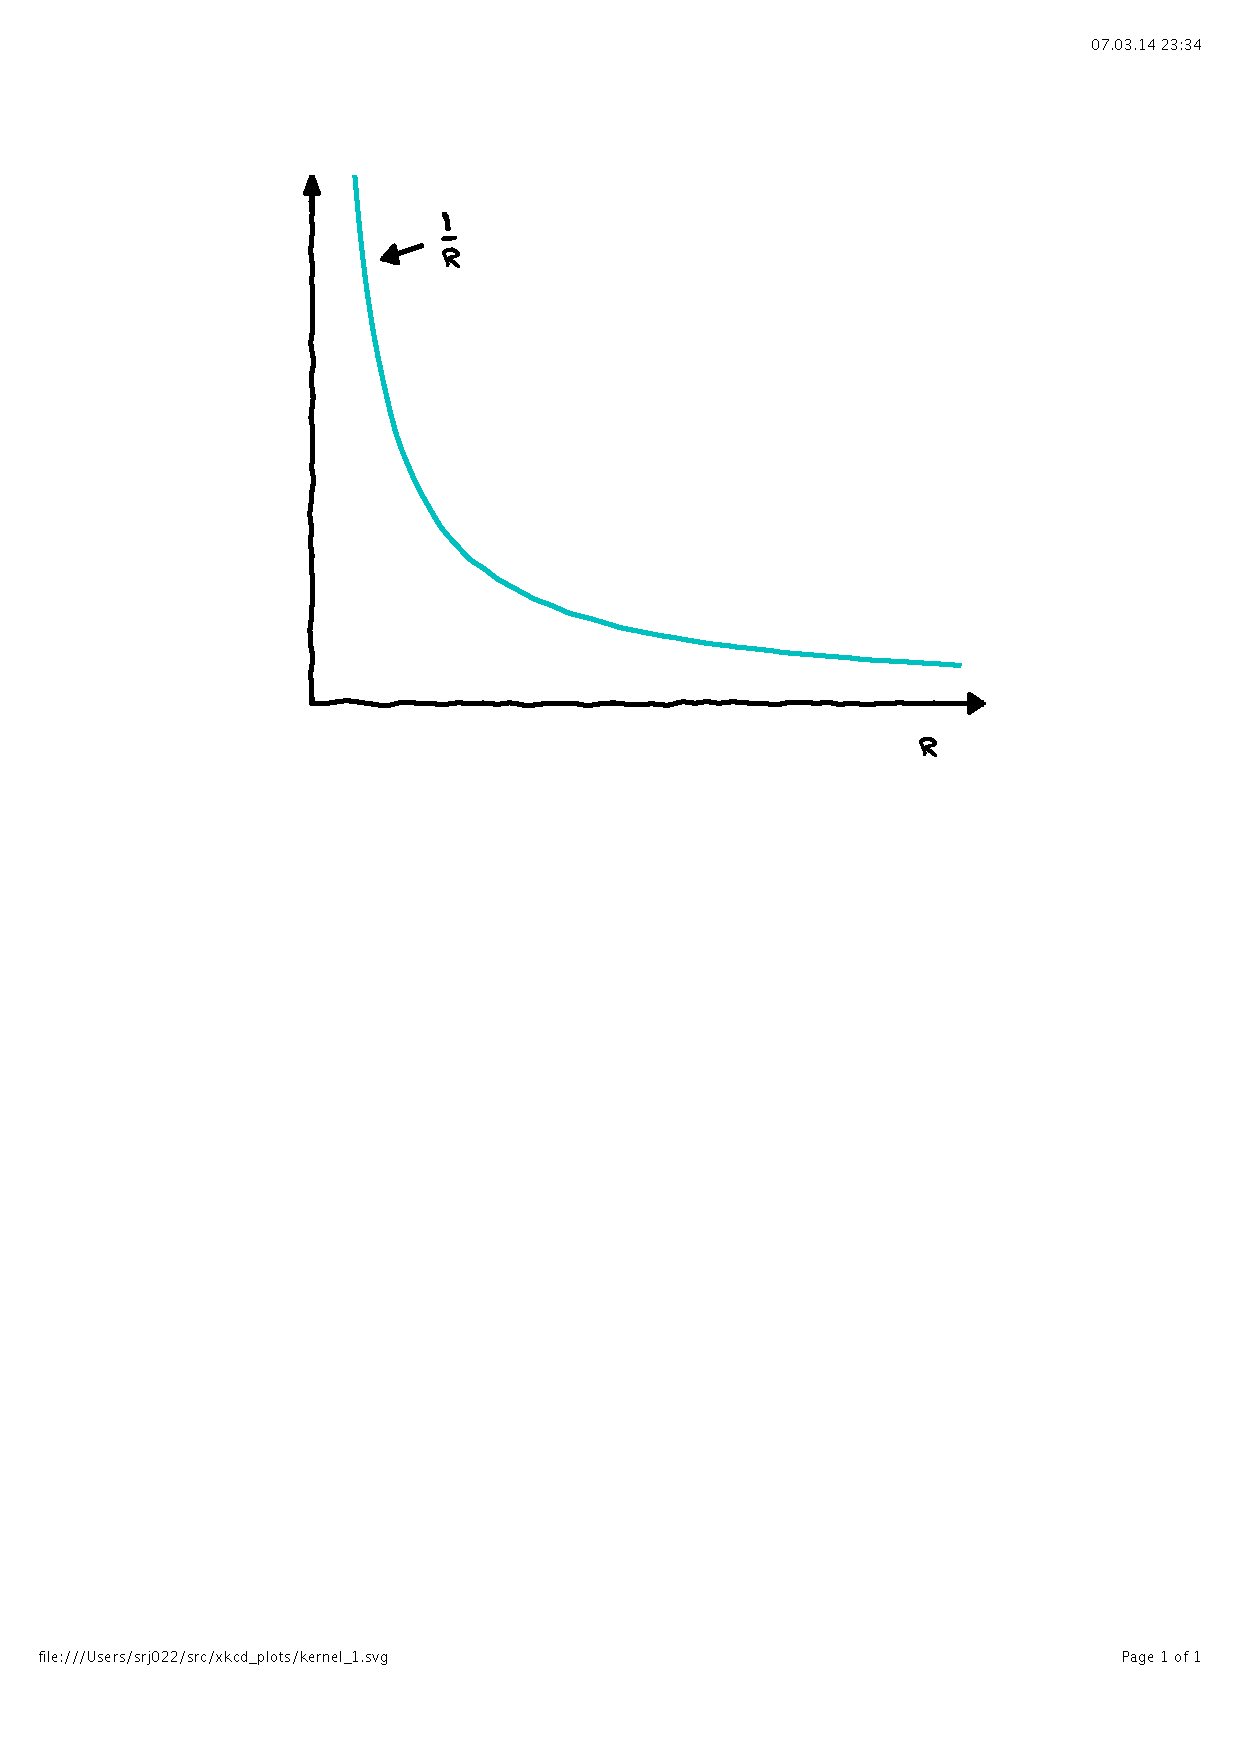
\includegraphics[scale=0.4, clip, viewport = 110 450 490 800]{figures/kernel_1.pdf}}
	\only<2>{\ \ \ \ \ \ 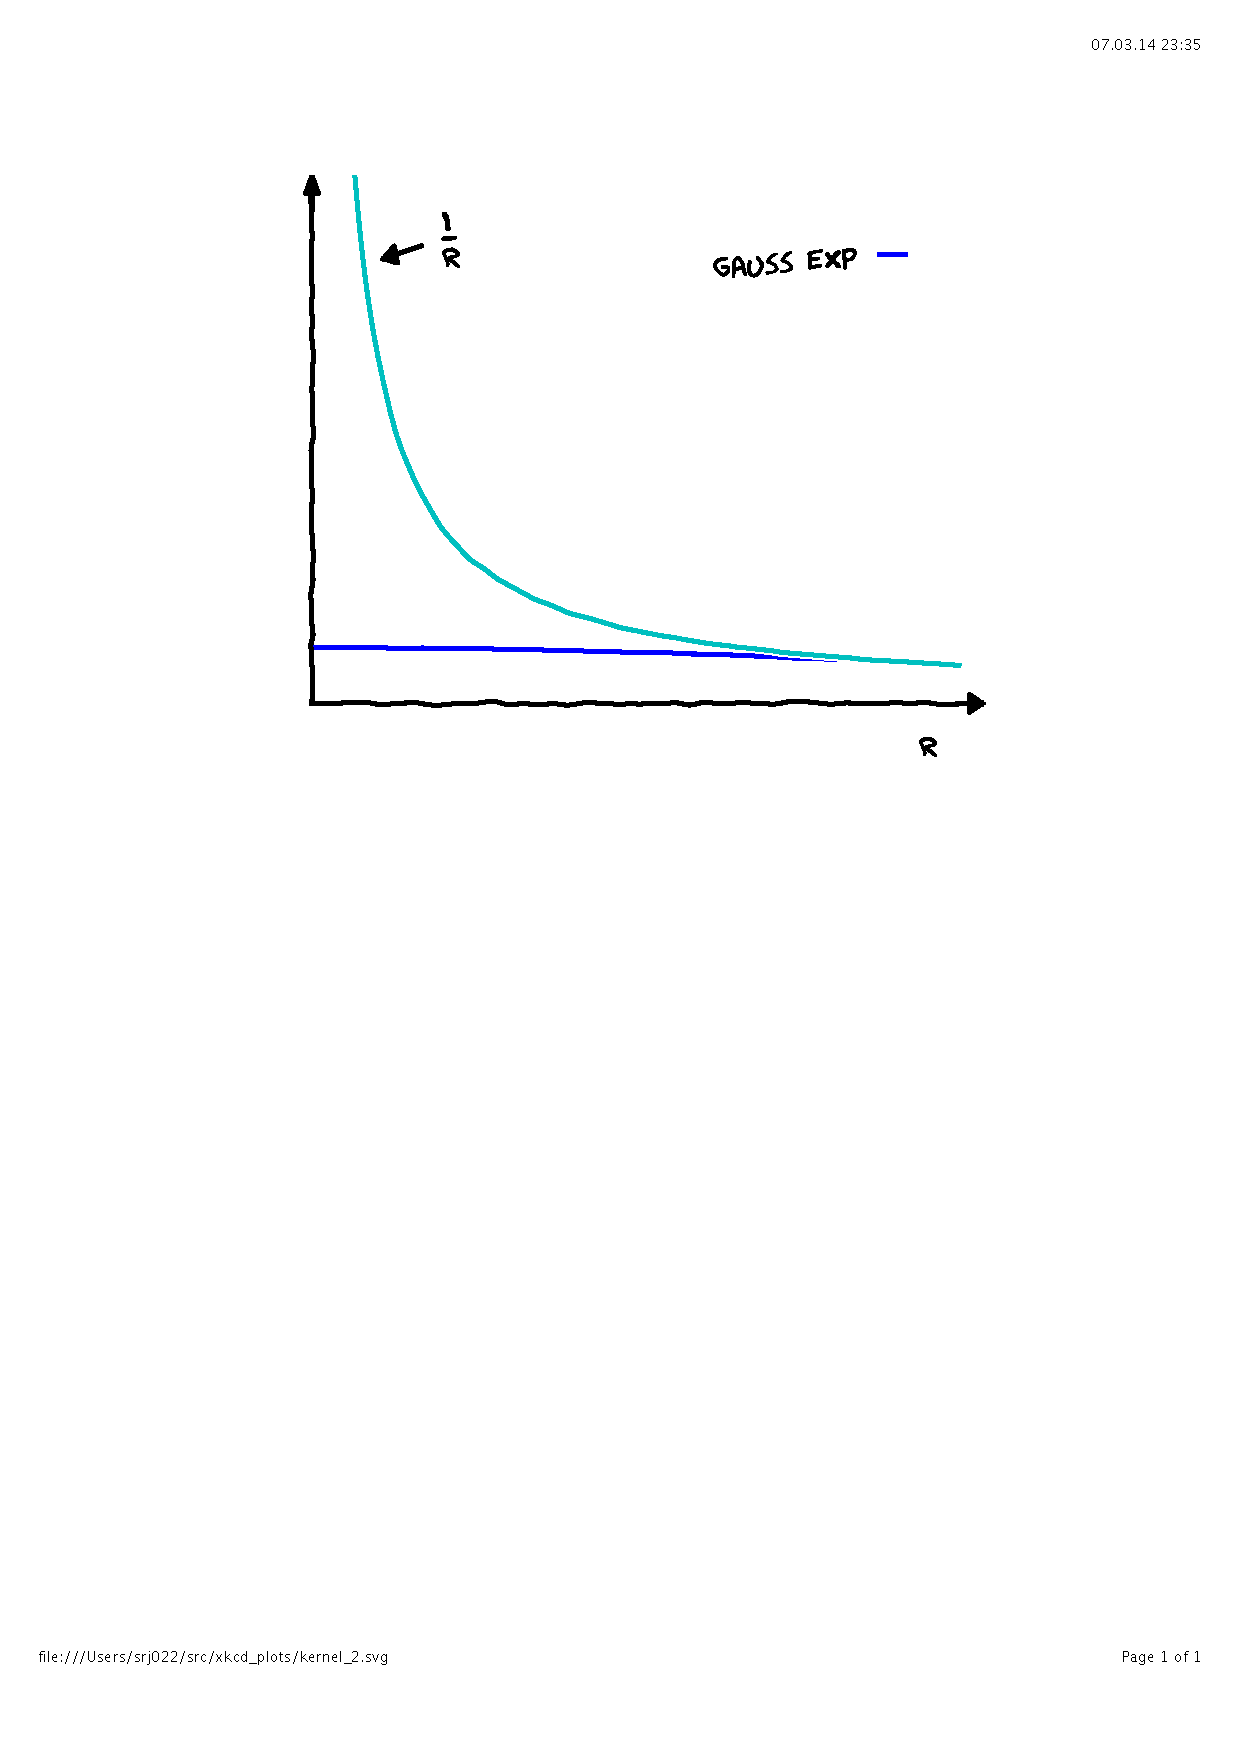
\includegraphics[scale=0.4, clip, viewport = 110 450 490 800]{figures/kernel_2.pdf}}
	\only<3>{\ \ \ \ \ 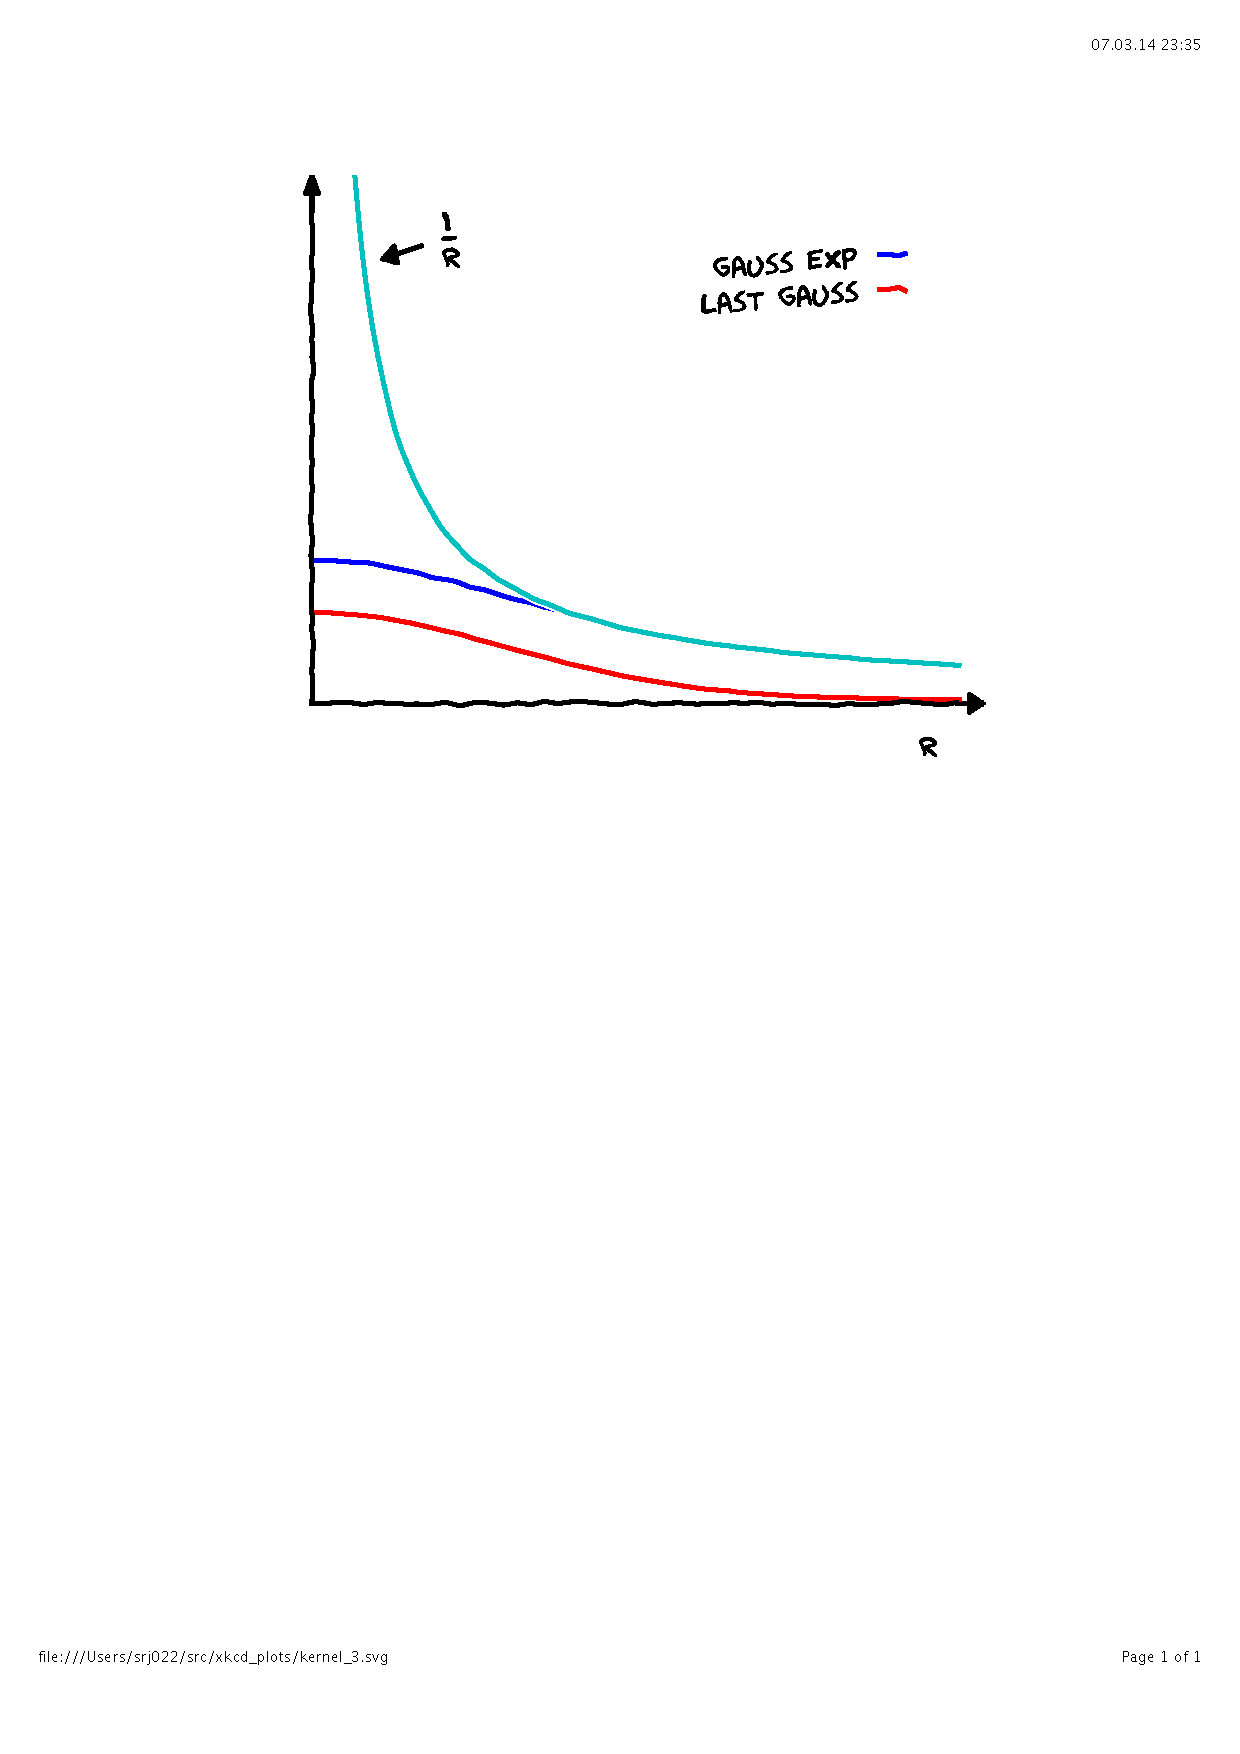
\includegraphics[scale=0.4, clip, viewport = 110 450 490 800]{figures/kernel_3.pdf}}
	\only<4>{\ \ \ \ 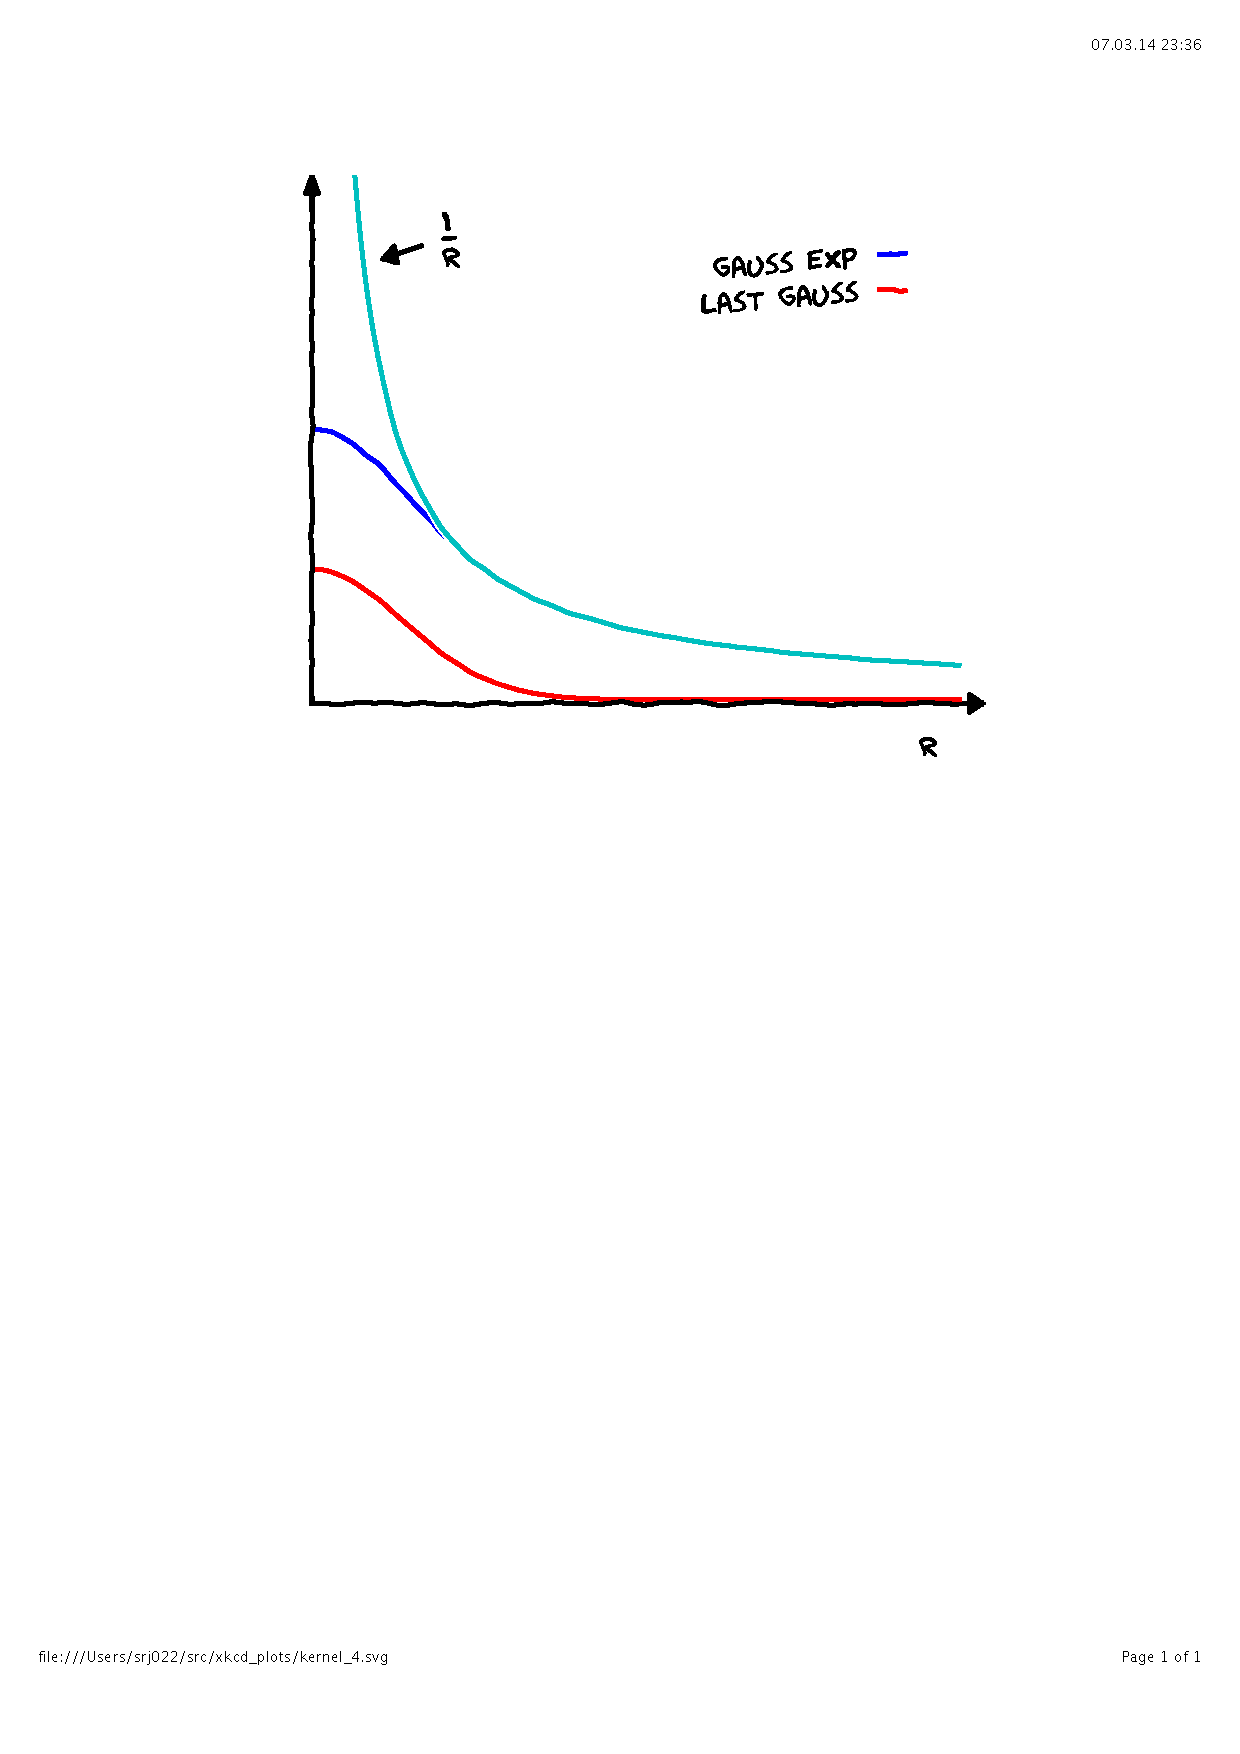
\includegraphics[scale=0.4, clip, viewport = 110 450 490 800]{figures/kernel_4.pdf}}
	\only<5>{\ \ \ 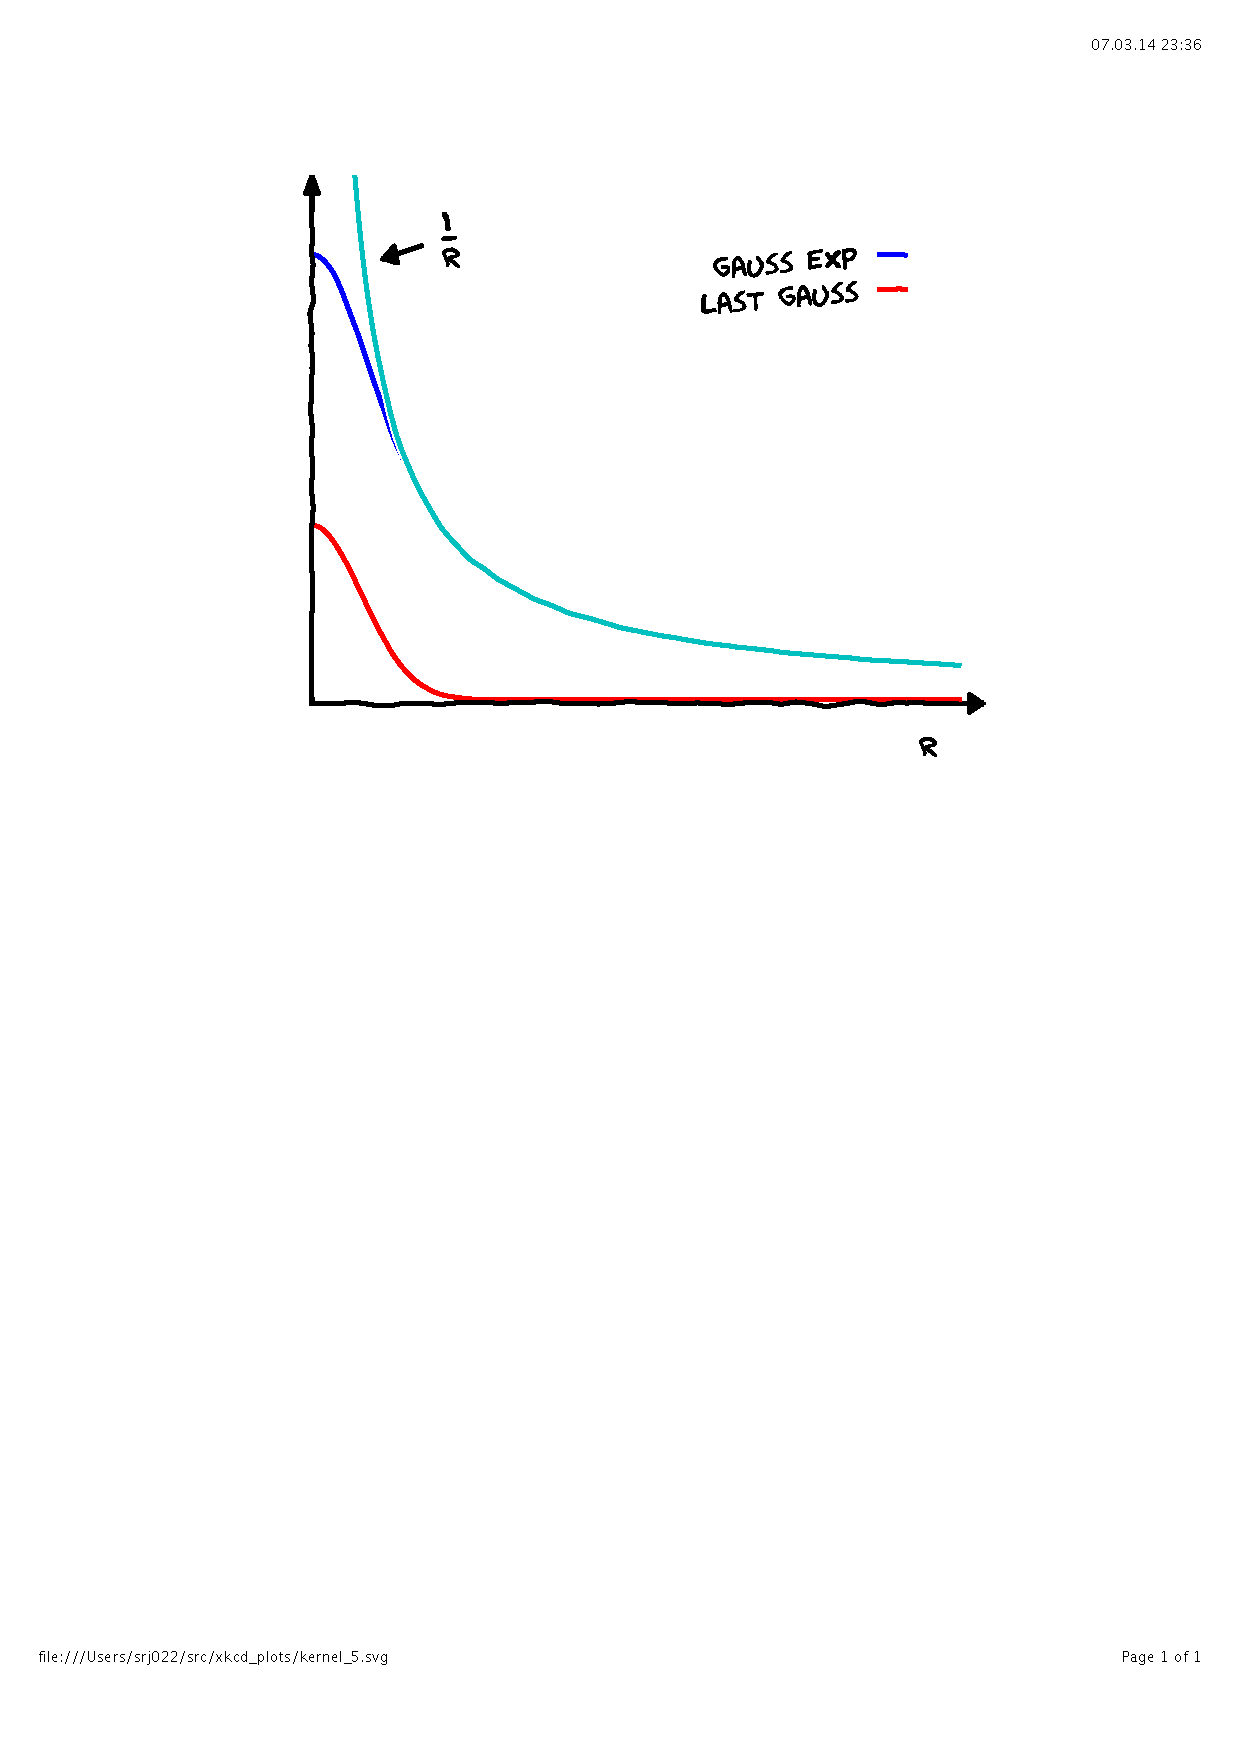
\includegraphics[scale=0.4, clip, viewport = 110 450 490 800]{figures/kernel_5.pdf}}
	\only<6>{\ \ 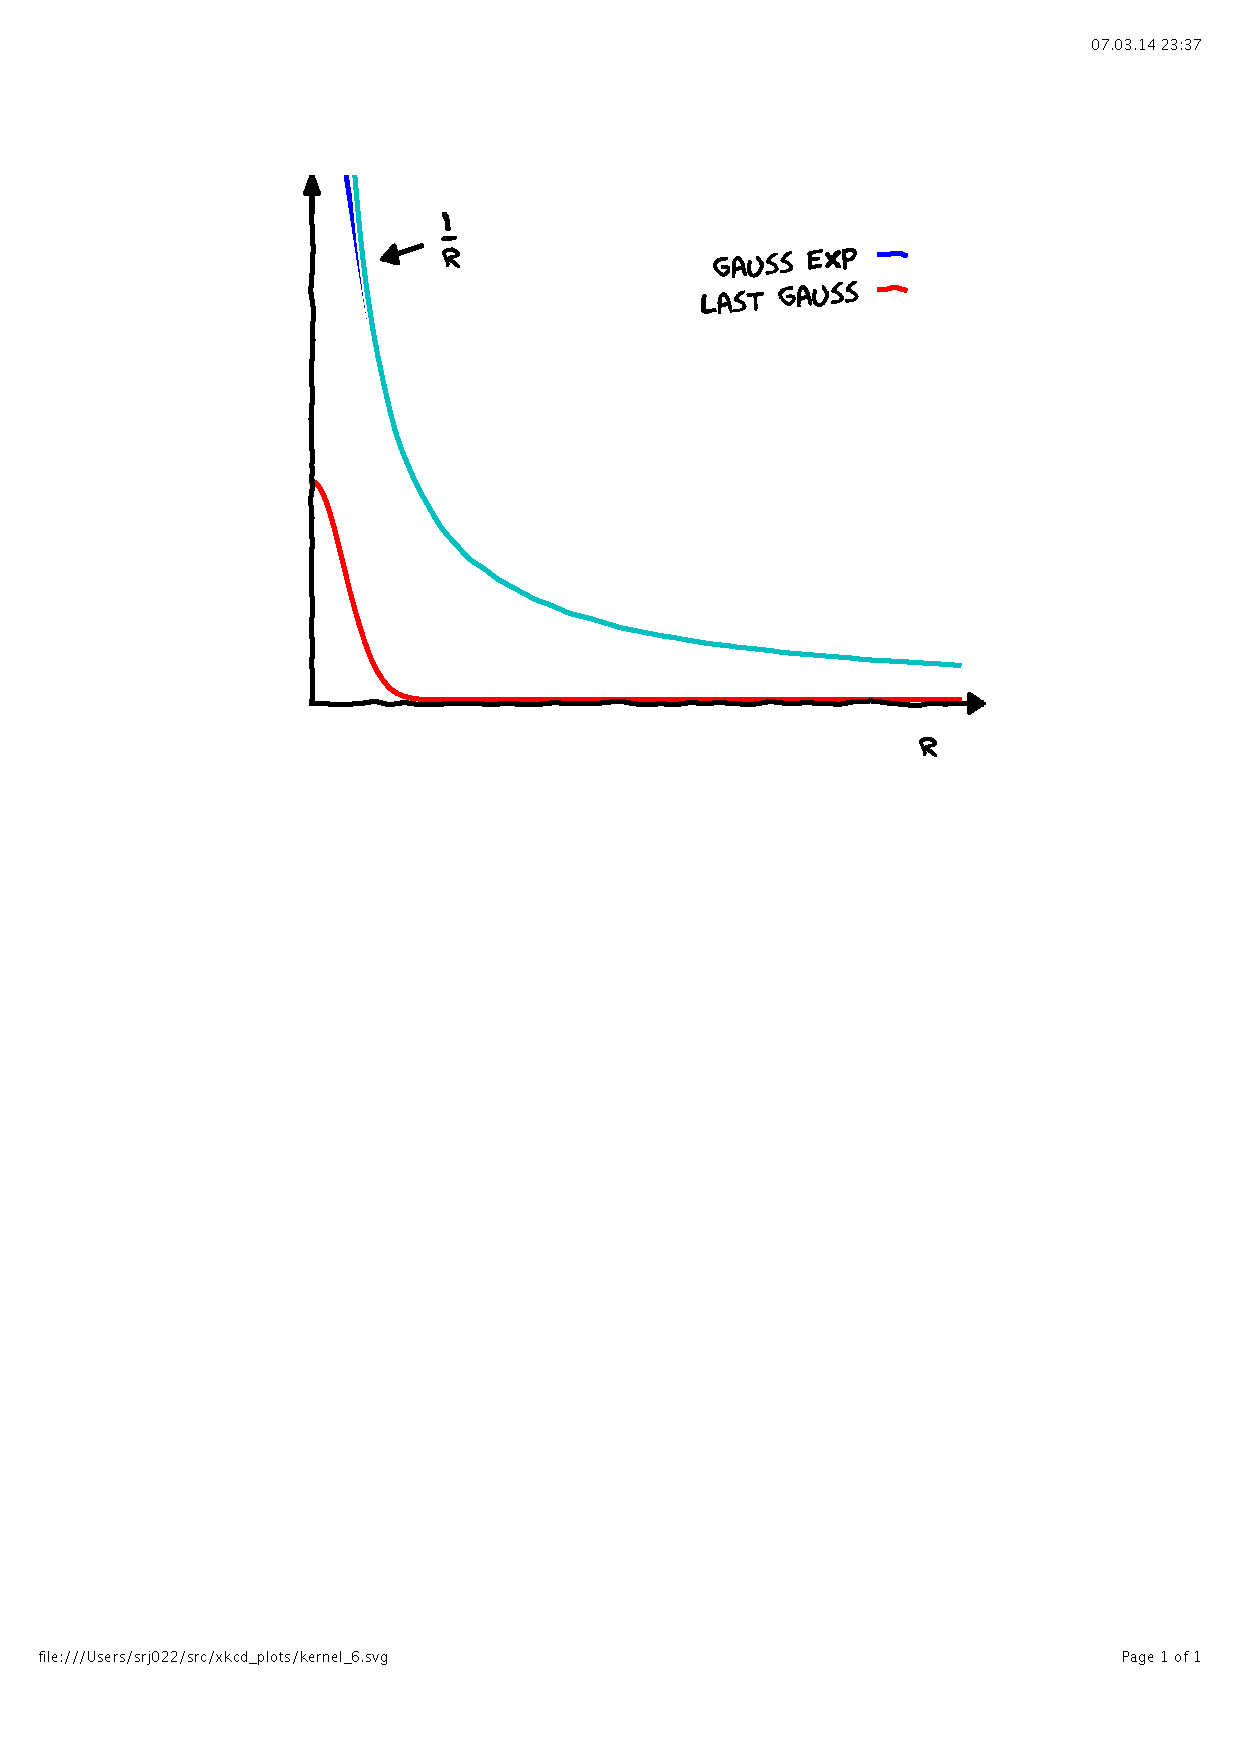
\includegraphics[scale=0.4, clip, viewport = 110 450 490 800]{figures/kernel_6.pdf}}
	\only<7,8>{\ 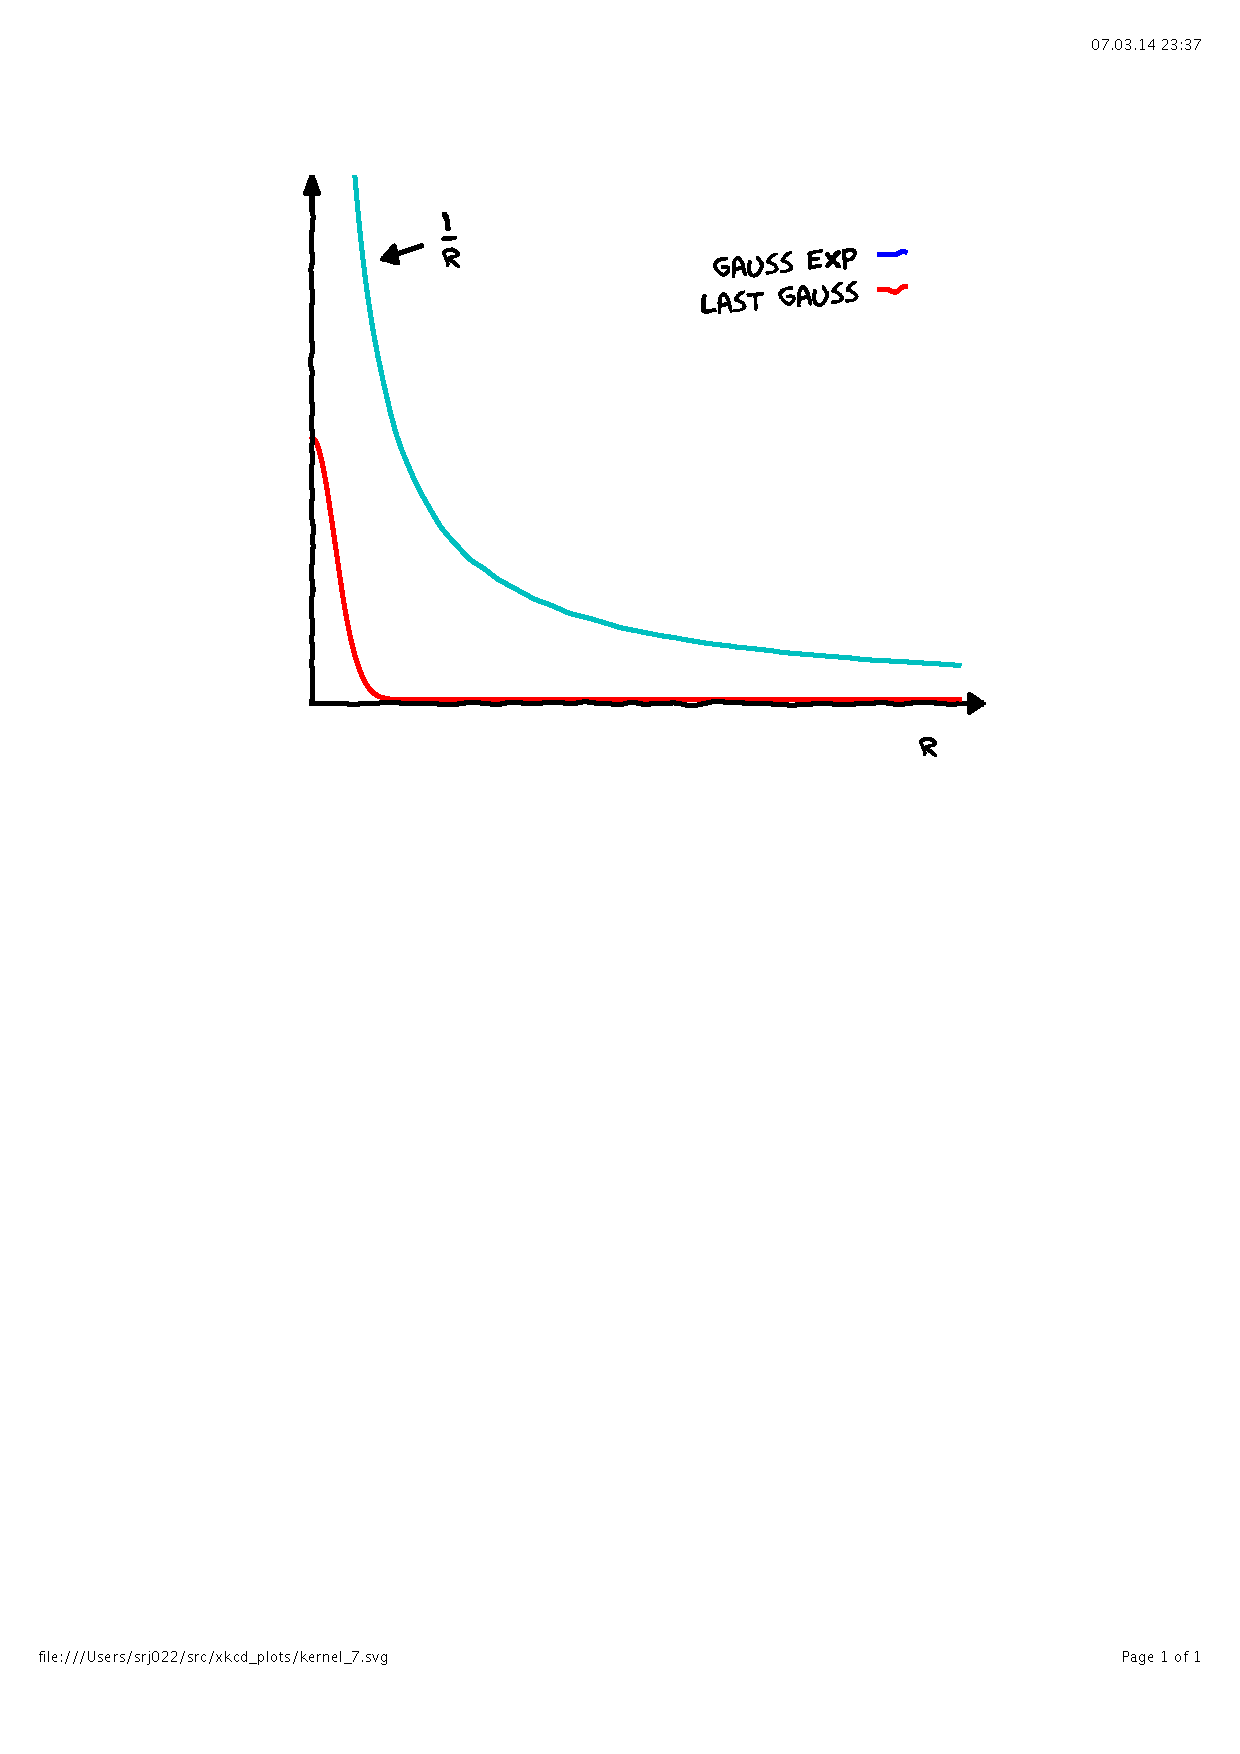
\includegraphics[scale=0.4, clip, viewport = 110 450 490 800]{figures/kernel_7.pdf}}
    \end{column}
    \end{columns}    
    \ \\
    \ \\
    \ \\
    \ \\
    \ \\
    \ \\
    \centering
    \only<1,2,3,4,5,6,7>{\ \\ \ \\}
    \only<8>{\normalsize{Combined with the sparse wavelet representation of operators we get\\
	\textbf{linear scaling algorithms}}}
\end{frame}

%\begin{frame}
    %\frametitle{Vanishing moments}
    %\centering
    %\textbf{A function $f$ has $M$ vanishing moments if}
    %\begin{equation}
	%\nonumber
	%\mu_m = \int_0^1 x^m f(x) dx = 0,\qquad m = 0, 1, \dots, M - 1
    %\end{equation}
    %\ \\
    %\ \\
    %\ \\
    %\begin{columns}
    %\begin{column}{.15\textwidth}
	%\ \\
    %\end{column}
    %\begin{column}{.85\textwidth}
    %\begin{itemize}
        %\item   Scaling basis has no vanishing moments $\longrightarrow$ \textbf{long ranged} interaction
        %\item   Wavelet basis has $k$ vanishing moments $\longrightarrow$ \textbf{short ranged} interaction
    %\end{itemize}
    %\end{column}
    %\end{columns}
    %\ \\
    %\ \\
    %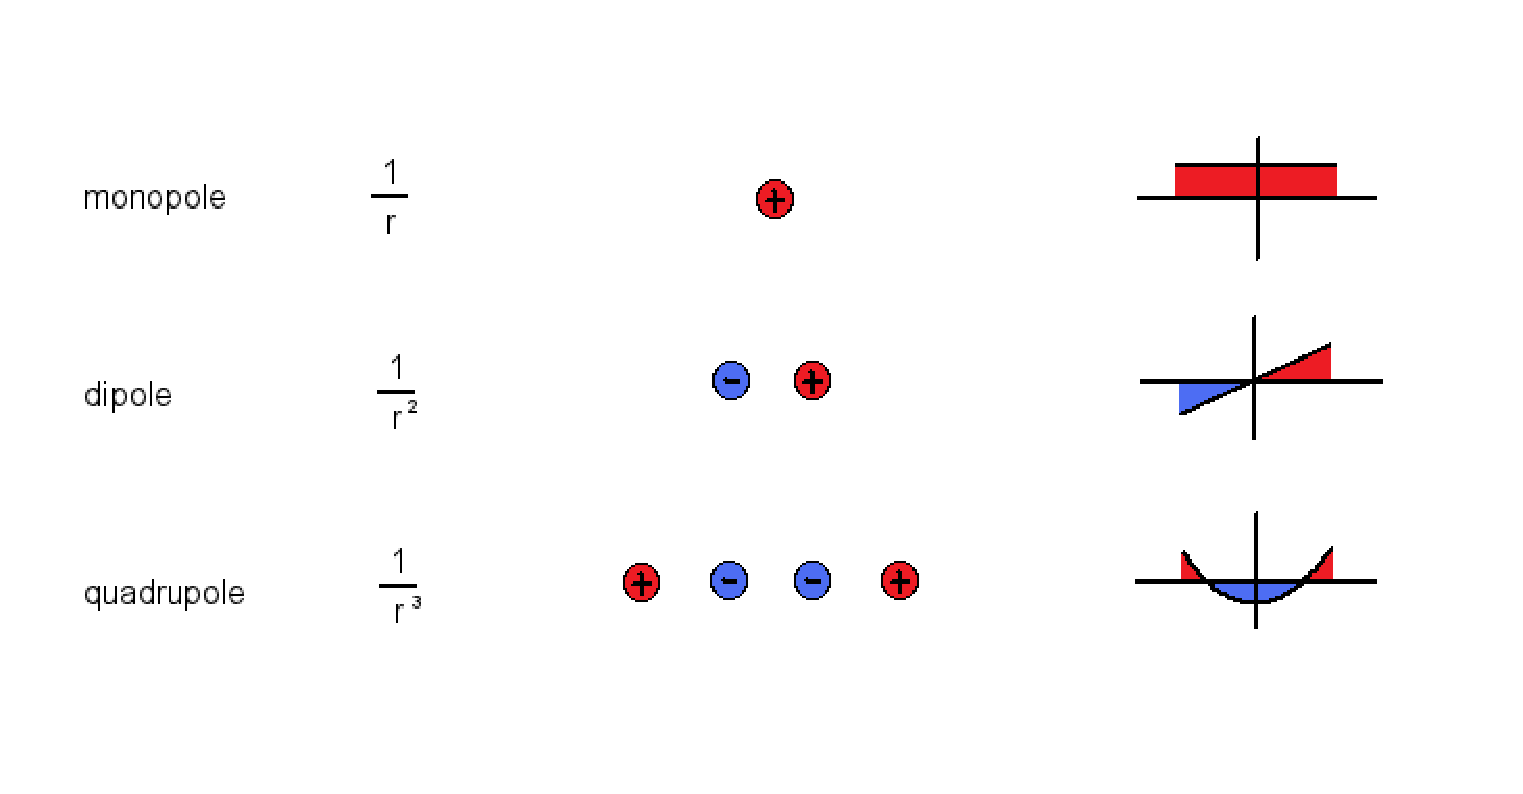
\includegraphics[scale=0.3, clip, viewport = 0 50 680 350]{figures/multipoles.pdf}
%\end{frame}

\begin{frame}
    \frametitle{Algorithm}
    \begin{algorithmic}[1]
	\STATE create \tree skeleton of empty \nodes for the output function
	\STATE create list of \emph{all} output \nodes
	\WHILE{number of output \nodes in the current list $N>0$}
	    \FOR{each output \node in the current list}
		\STATE fetch \emph{all} input \nodes within bandwidth of the \emph{full} operator
		\STATE compute scaling and wavelet coefficients of output \node
	    \ENDFOR
	    \FOR{each \node of the output function}
		\STATE remove \node from current list
		\IF{\node needs to be refined}
		    \STATE allocate children \nodes
		    \STATE add children \nodes to the current list
		\ENDIF
	    \ENDFOR
	\ENDWHILE
    \end{algorithmic}
    \ \\
    \ \\
    \ \\
    \pause
    \begin{algorithmic}[1]
	\FOR{each separated component ($\kappa = 1,\dots,M$) of the operator}
	    \FOR{each s/w component of output function}
		\FOR{each s/w component of input function}
		    \STATE fetch appropriate operator component (e.g. $T\times A\times A$)
		    \STATE construct bandwidth
		    \STATE fetch input and operator \nodes within bandwidth
		    \STATE prune list of input \nodes based on Cauchy-Schwartz screening
		    \FOR{each contributing input \node}
			\STATE apply operator
		    \ENDFOR
		\ENDFOR
	    \ENDFOR
	\ENDFOR		
    \end{algorithmic}
\end{frame}

\begin{frame}
    \frametitle{Linear scaling Coulomb interaction}
    \begin{columns}
    \begin{column}{.10\textwidth}
    \ \\
    \end{column}
    \begin{column}{.40\textwidth}
	\centering
	\ \\
	\ \\
	\ \\
	\ \\
	\textbf{Alkane chains}
	\begin{equation}
	    \nonumber
	    C_{n}H_{2n+2}, \qquad n=2,\dots,70
	\end{equation}
	\ \\
	\ \\
	\ \\
	\ \\
	\textbf{Fitted curve}
	\begin{equation}
	    \nonumber
	    t_{rel}(n) = 12.5 + 2.34n^{0.754} 
	\end{equation}
    \end{column}
    \begin{column}{.50\textwidth}
	\centering
	\begin{figure}
	    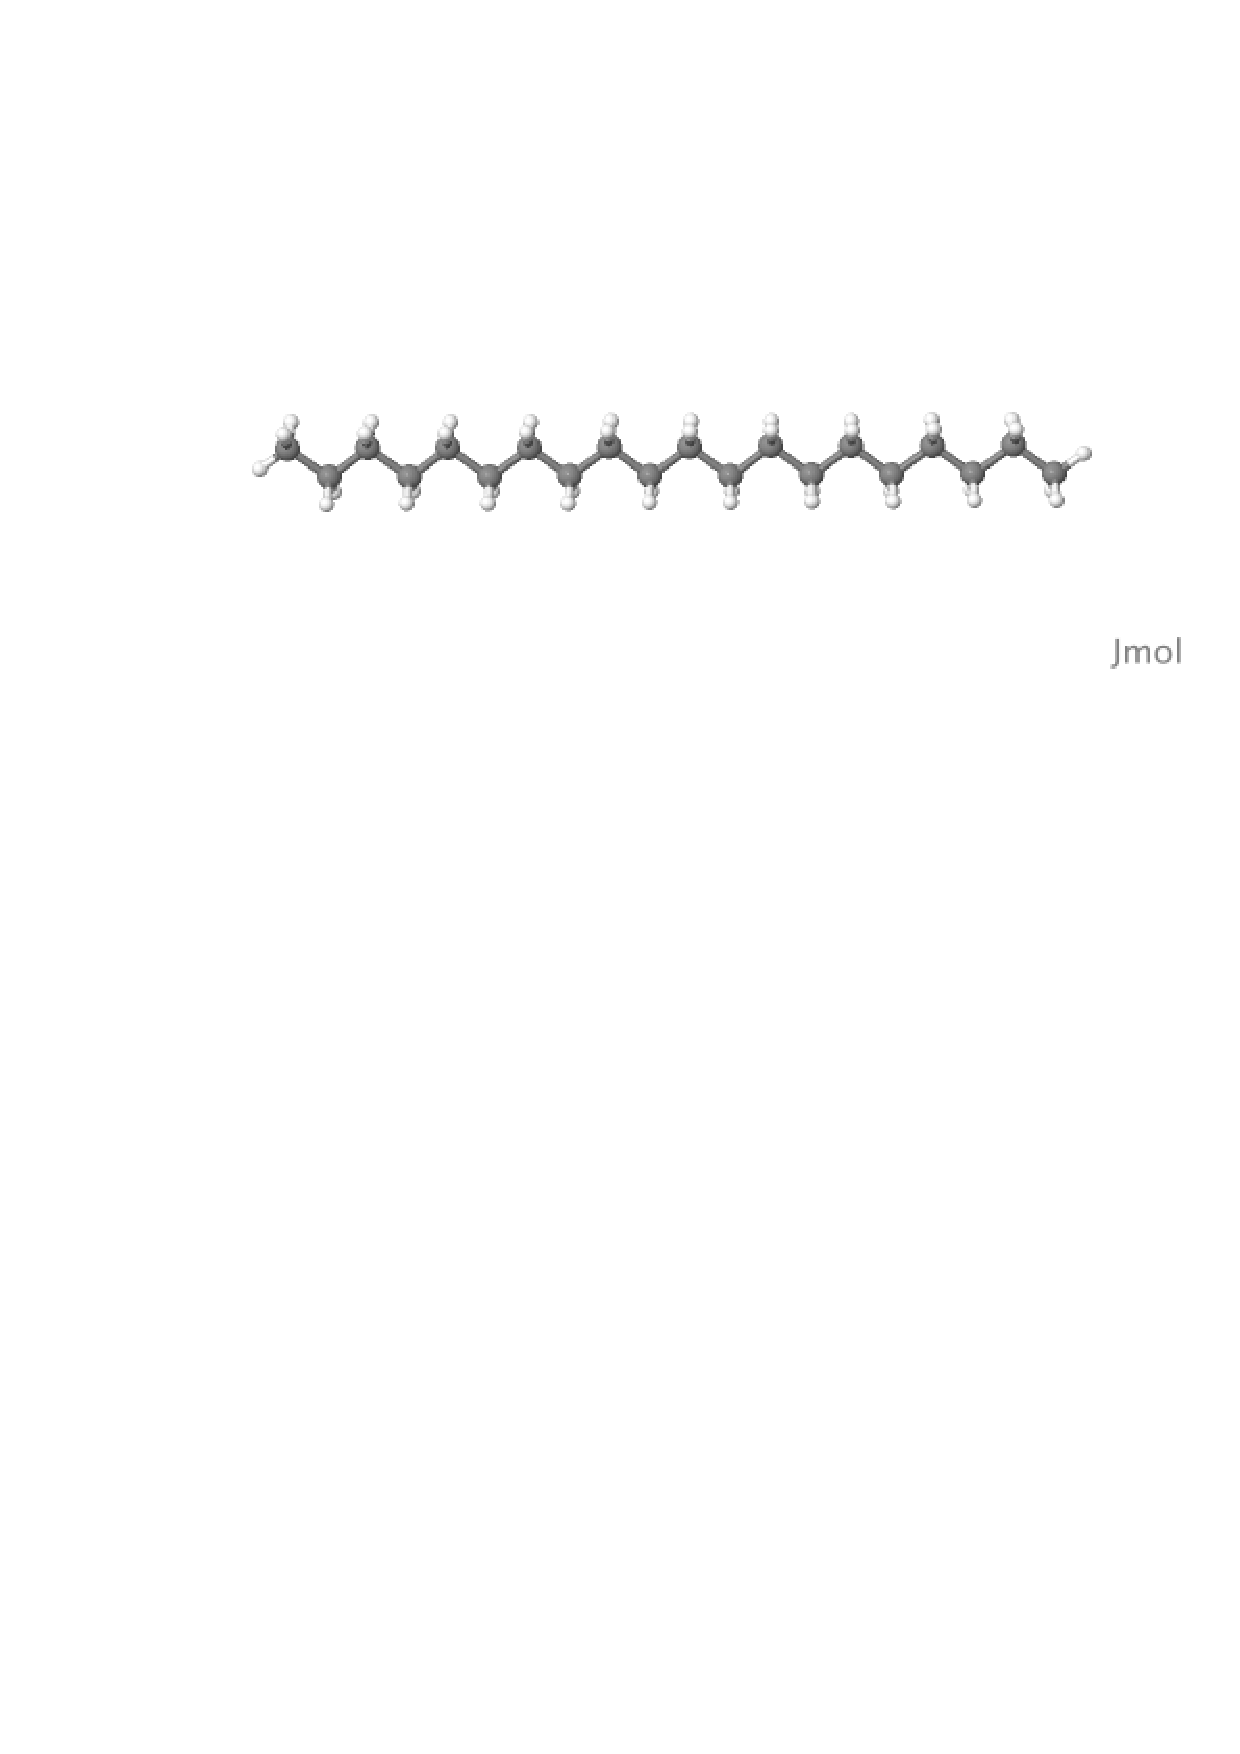
\includegraphics[scale=0.3, clip, viewport = 80 560 600 720]{figures/alkane.pdf}
	\end{figure}
	\textbf{Fitted curve}
	\begin{equation}
	    \nonumber
	    t_{abs}(n) = -6.0 + 1.33n^{0.991}
	\end{equation}
	\ \\
	\ \\
    \end{column}
    \end{columns}    
    \ \\
    \begin{center}
	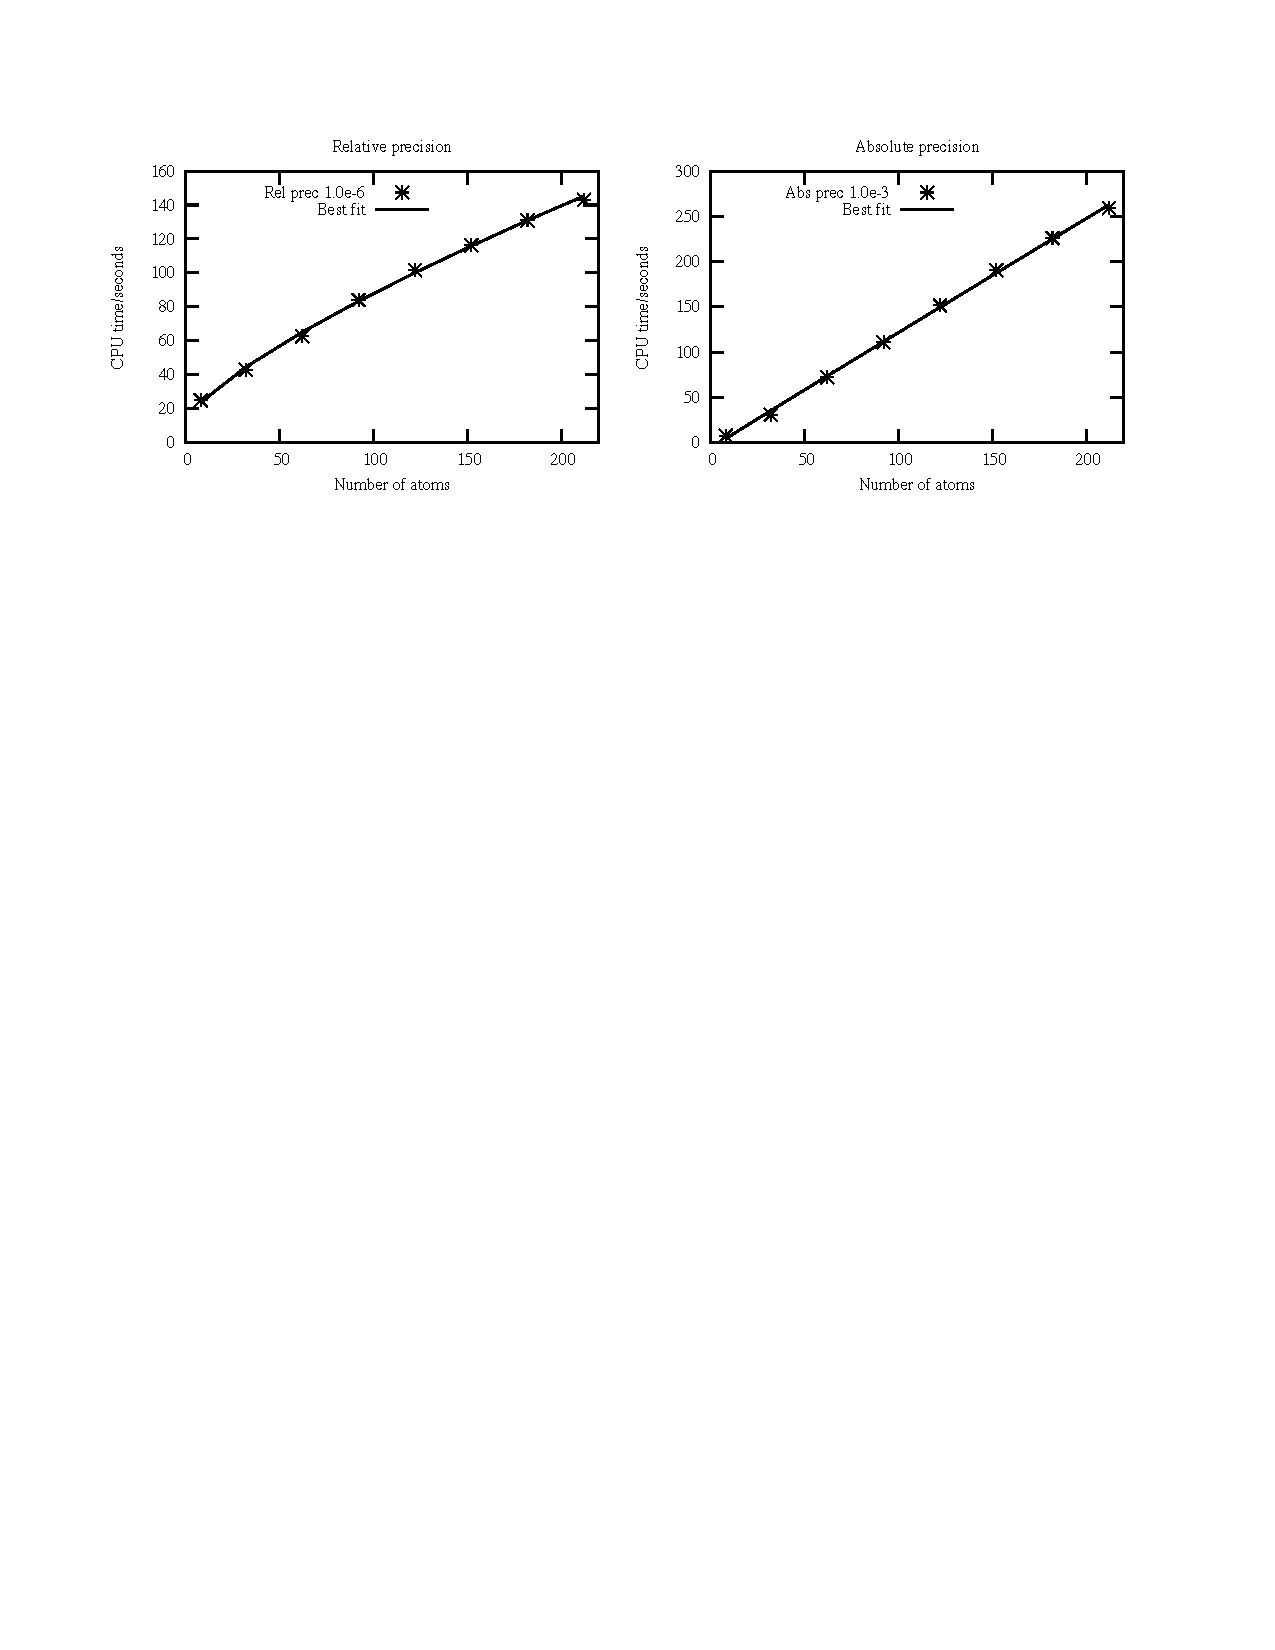
\includegraphics[scale=0.6, clip, viewport = 50 550 540 730]{figures/linearScaling.pdf}
    \end{center}
\end{frame}

%\begin{frame}
    %\frametitle{Parallel programming}
    %Why parallel processing?
    %\begin{itemize}
	%\item	To get more processing power
	%\item	To get more available memory
	%\item	Future $\rightarrow$ \emph{more} processors rather than faster
    %\end{itemize}
    %\ \\
    %\ \\
    %\ \\
    %\pause
    %Parallelization means
    %\begin{itemize}
	%\item	\textbf{distributing work} among available processors
	%\item	\textbf{syncronizing} distributed work
	%\item	\textbf{distributing data} among available memory
	%\item	\textbf{communicating} distributed data
    %\end{itemize}
%\end{frame}

%\begin{frame}
    %\frametitle{Shared memory (OpenMP)}
    %\begin{columns}
    %\begin{column}[b]{0.45\linewidth}
	%Pros
	%\begin{itemize}
	    %\item Relatively simple implementation
	    %\item Quick way to good performance
	    %\item No communication
	    %\item Simple load balance
	%\end{itemize}
	%\ \\
	%\ \\
	%\pause
	%Cons
        %\begin{itemize}
	    %\item Small to medium scale parallelization
	    %\item Limited memory
	    %\item Race conditions
	    %\item Tedious debugging (Heisenbugs)
	%\end{itemize}
	%\ \\
	%\ \\
    %\end{column}
    %\begin{column}[b]{0.4\linewidth}
	%\only<3>{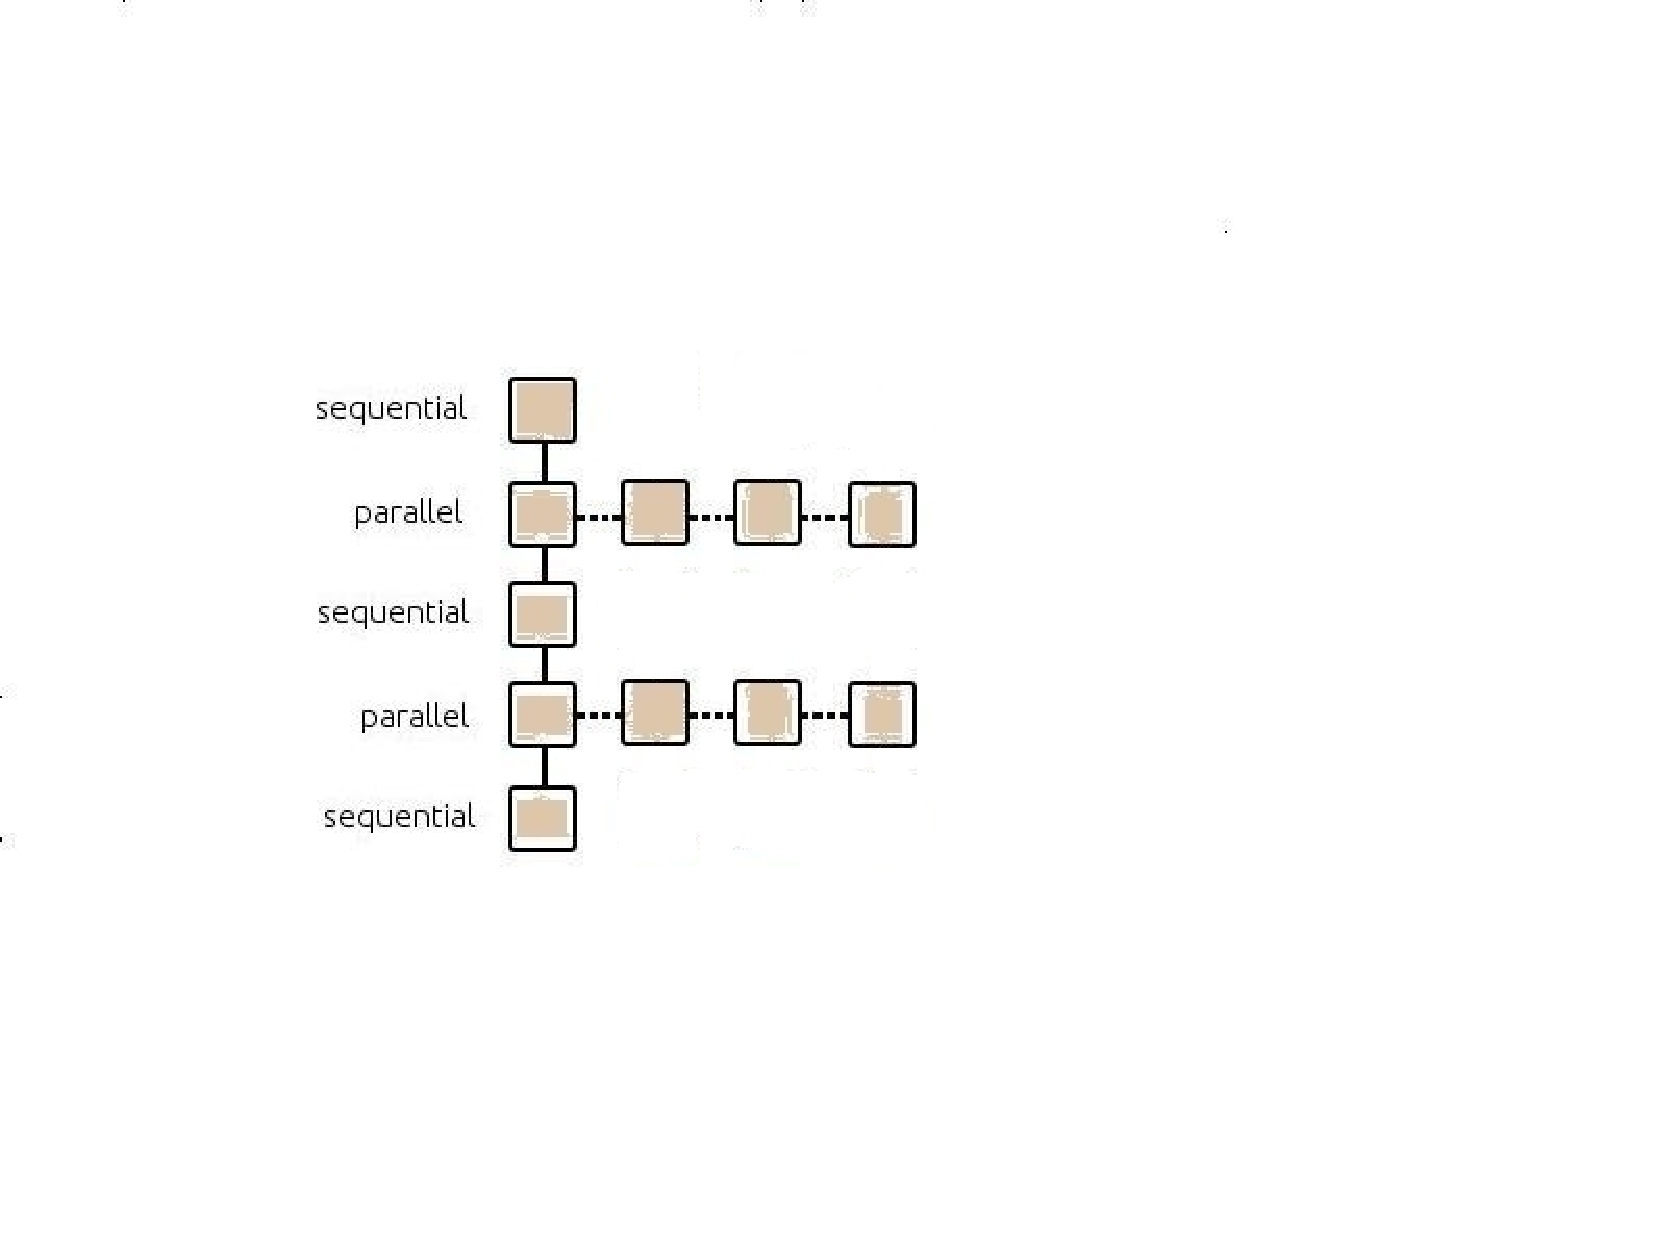
\includegraphics[viewport = 120 160 460 450, clip, scale=0.4]{figures/parallel_OMP.pdf}}
	%\ \\
	%\ \\
	%\ \\
	%\ \\
    %\end{column}
    %\end{columns}
%\end{frame}

%\begin{frame}
    %\frametitle{Distributed memory (MPI)}
    %\begin{columns}
    %\begin{column}[b]{0.45\linewidth}
	%Pros
	%\begin{itemize}
	    %\item Large scale parallelization
	    %\item Extensive memory
	%\end{itemize}
	%\ \\
	%\ \\
	%\ \\
	%\ \\
	%\pause
	%Cons
	%\begin{itemize}
	    %\item Complicated implementation
	    %\item User specified work/data decomposition 
	    %\item User specified communication
	    %\item Difficult to load balance
	    %\item Communication overhead
	%\end{itemize}
    %\end{column}
    %\begin{column}[b]{0.4\linewidth}
	%\only<3>{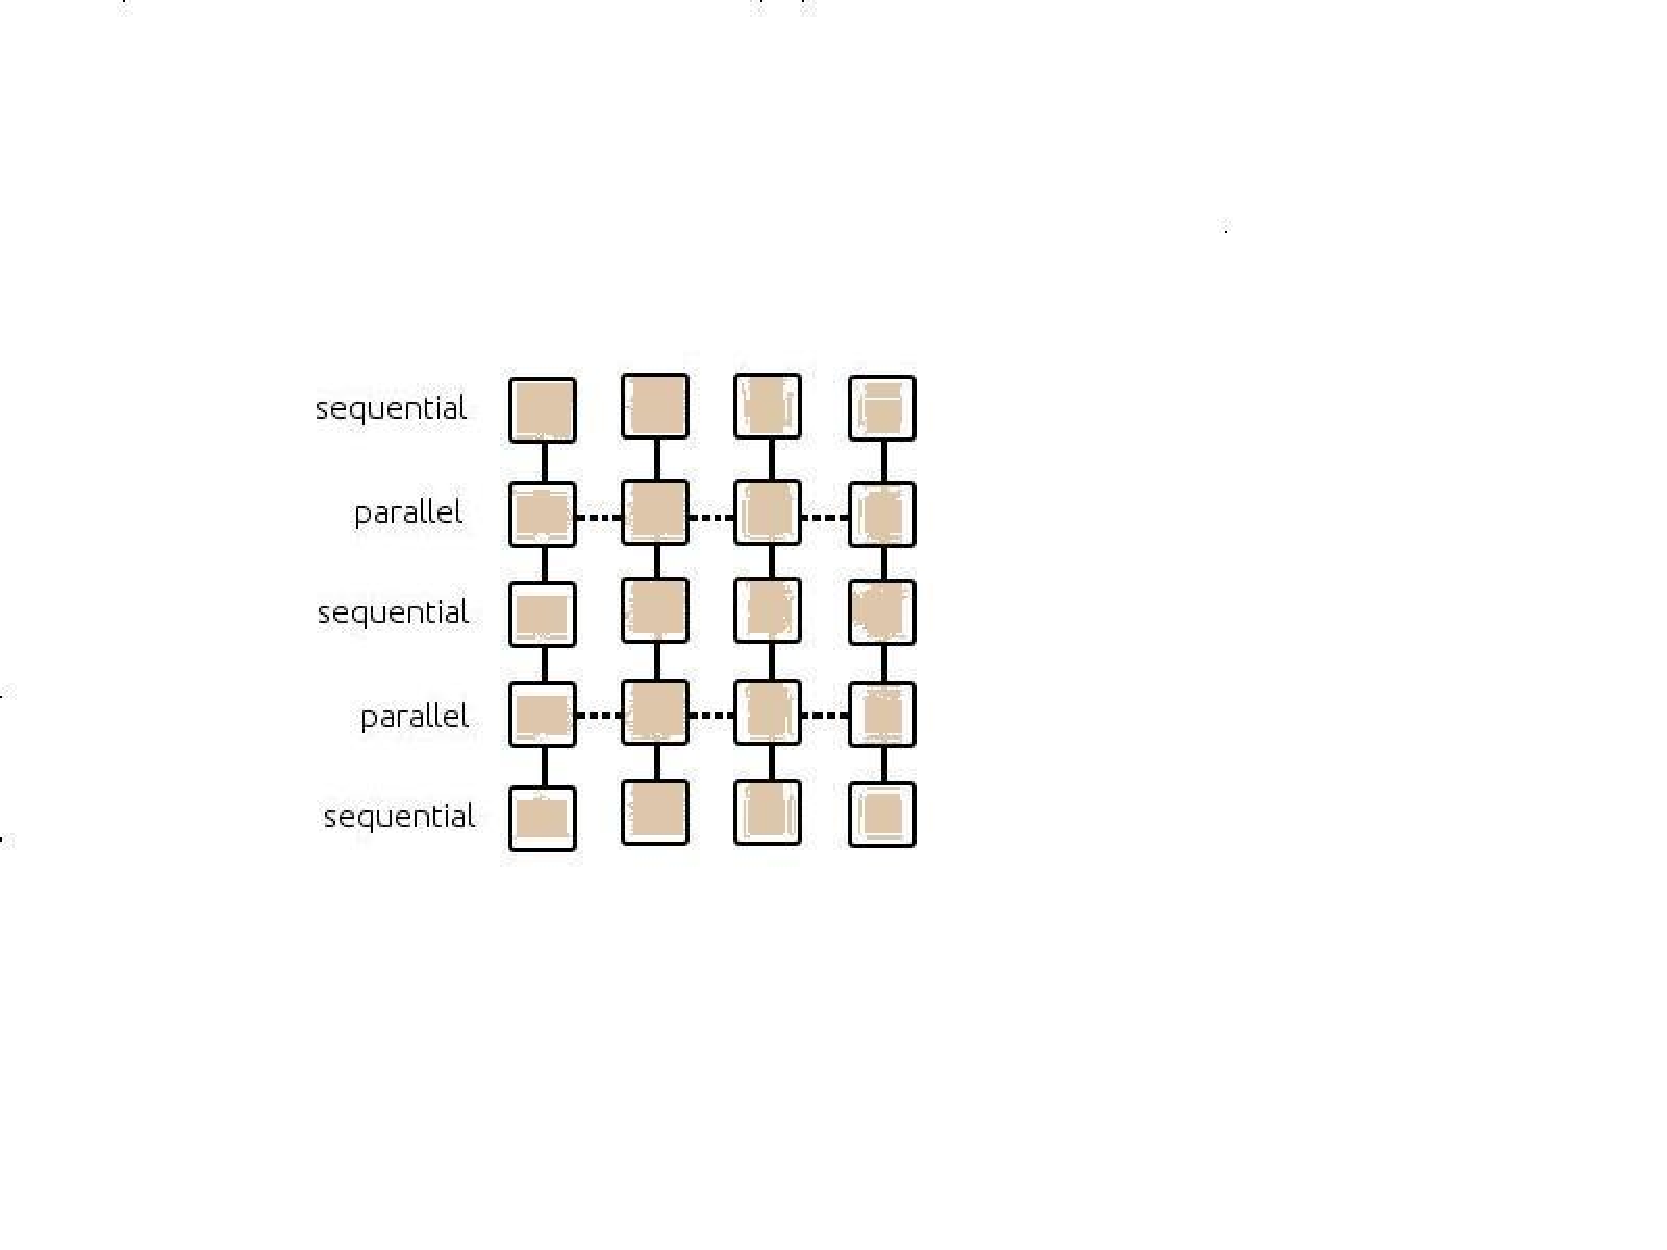
\includegraphics[viewport = 120 160 460 450, clip, scale=0.4]{figures/parallel_mpi_2.pdf}}
	%\ \\
	%\ \\
	%\ \\
    %\end{column}
    %\end{columns}
%\end{frame}

%\begin{frame}
    %\frametitle{Parallel efficiency}
    %\begin{center}
    %\only<1>{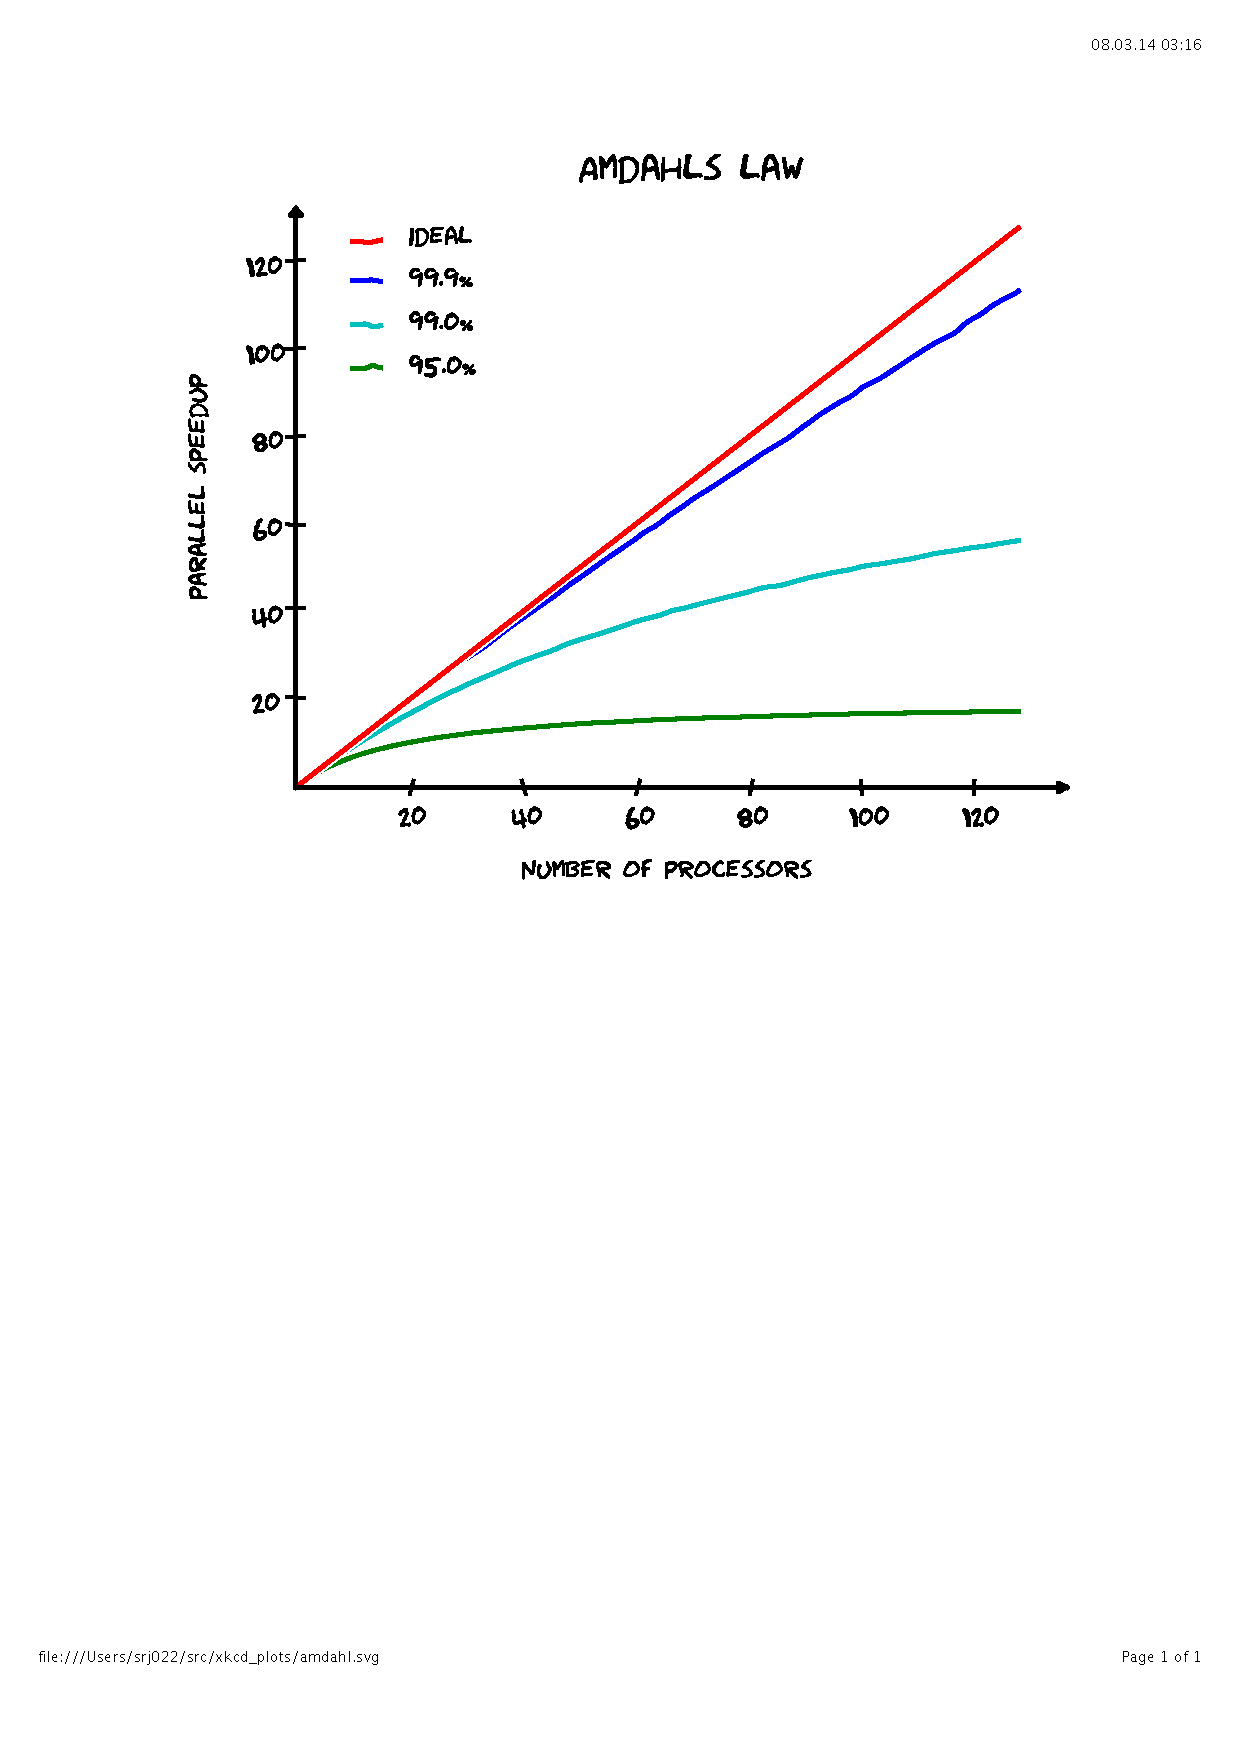
\includegraphics[clip, viewport = 50 250 550 800, scale=0.5]{figures/amdahl.pdf}}
    %\only<2>{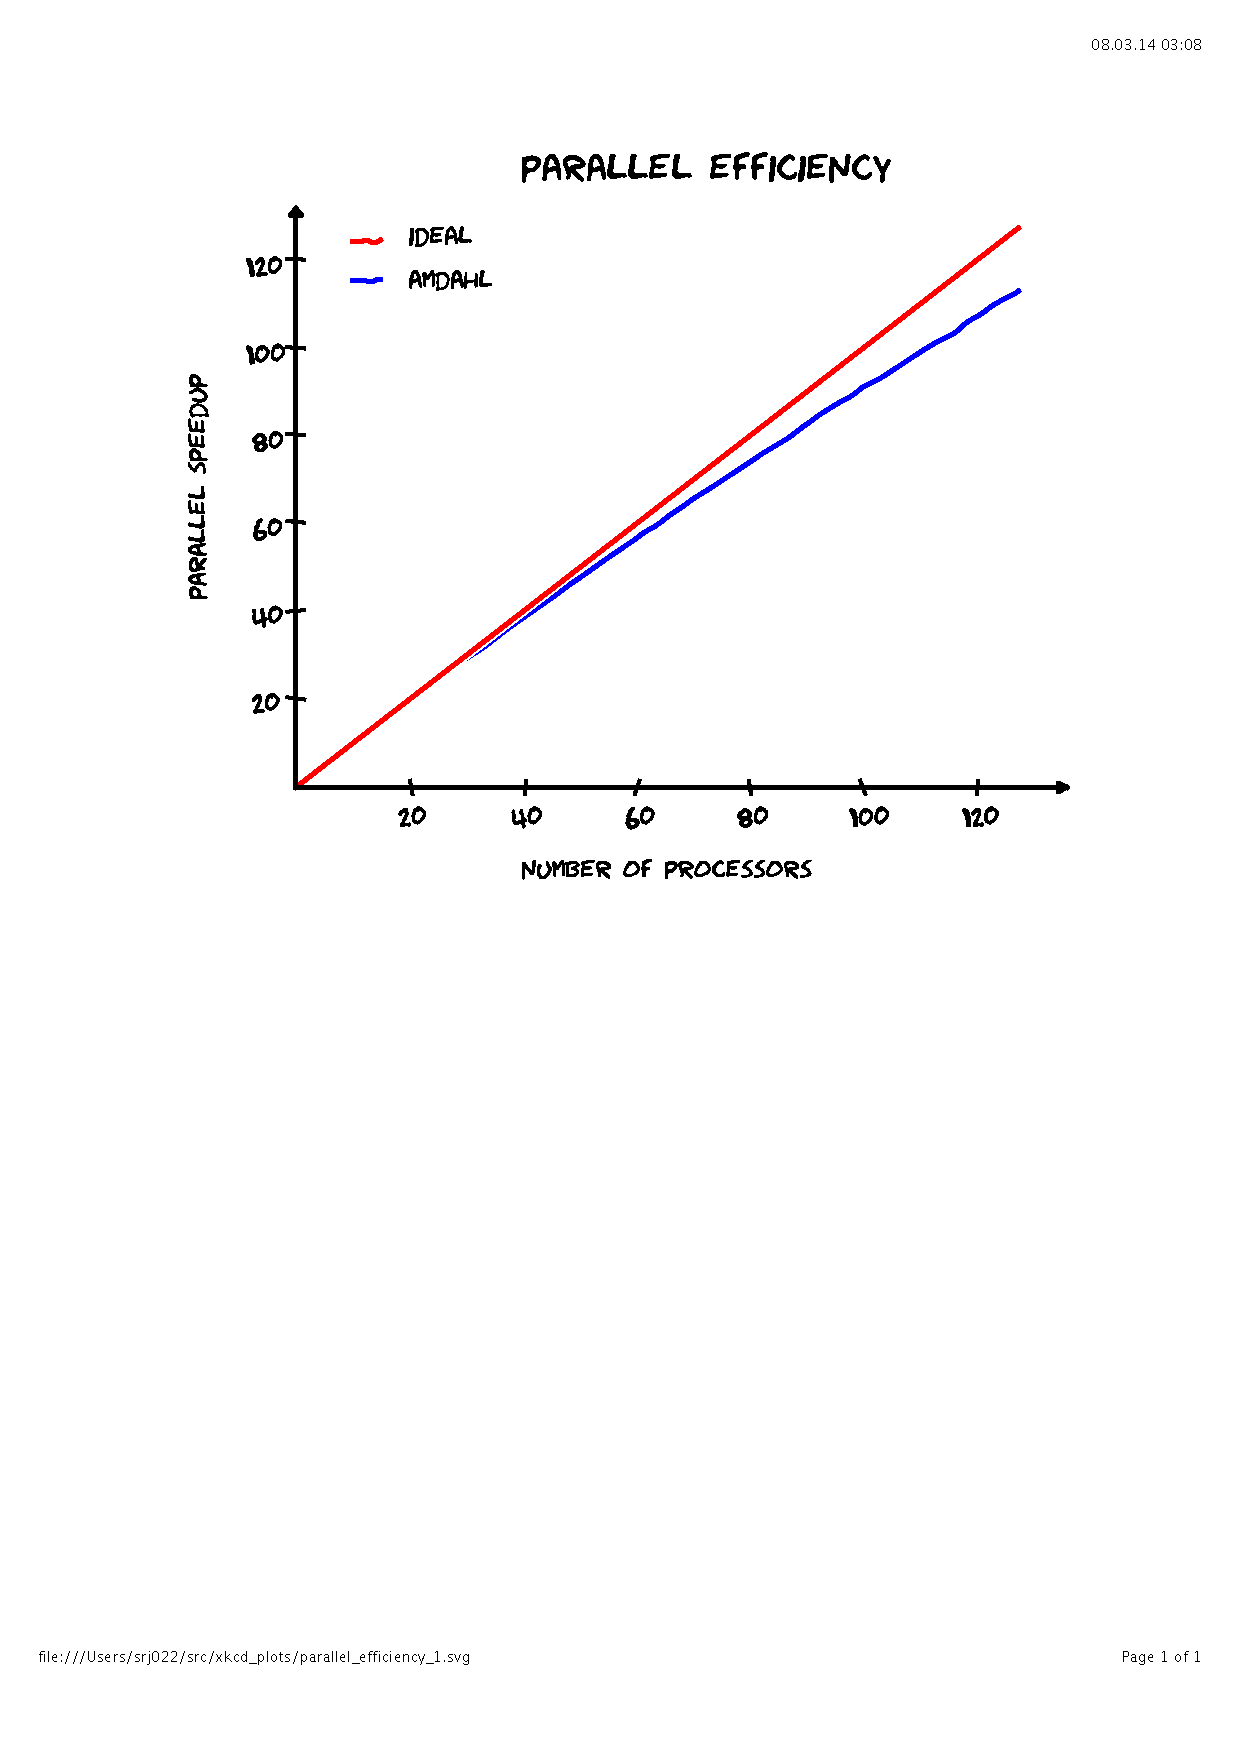
\includegraphics[clip, viewport = 50 250 550 800, scale=0.5]{figures/parallel_efficiency_1.pdf}}
    %\only<3>{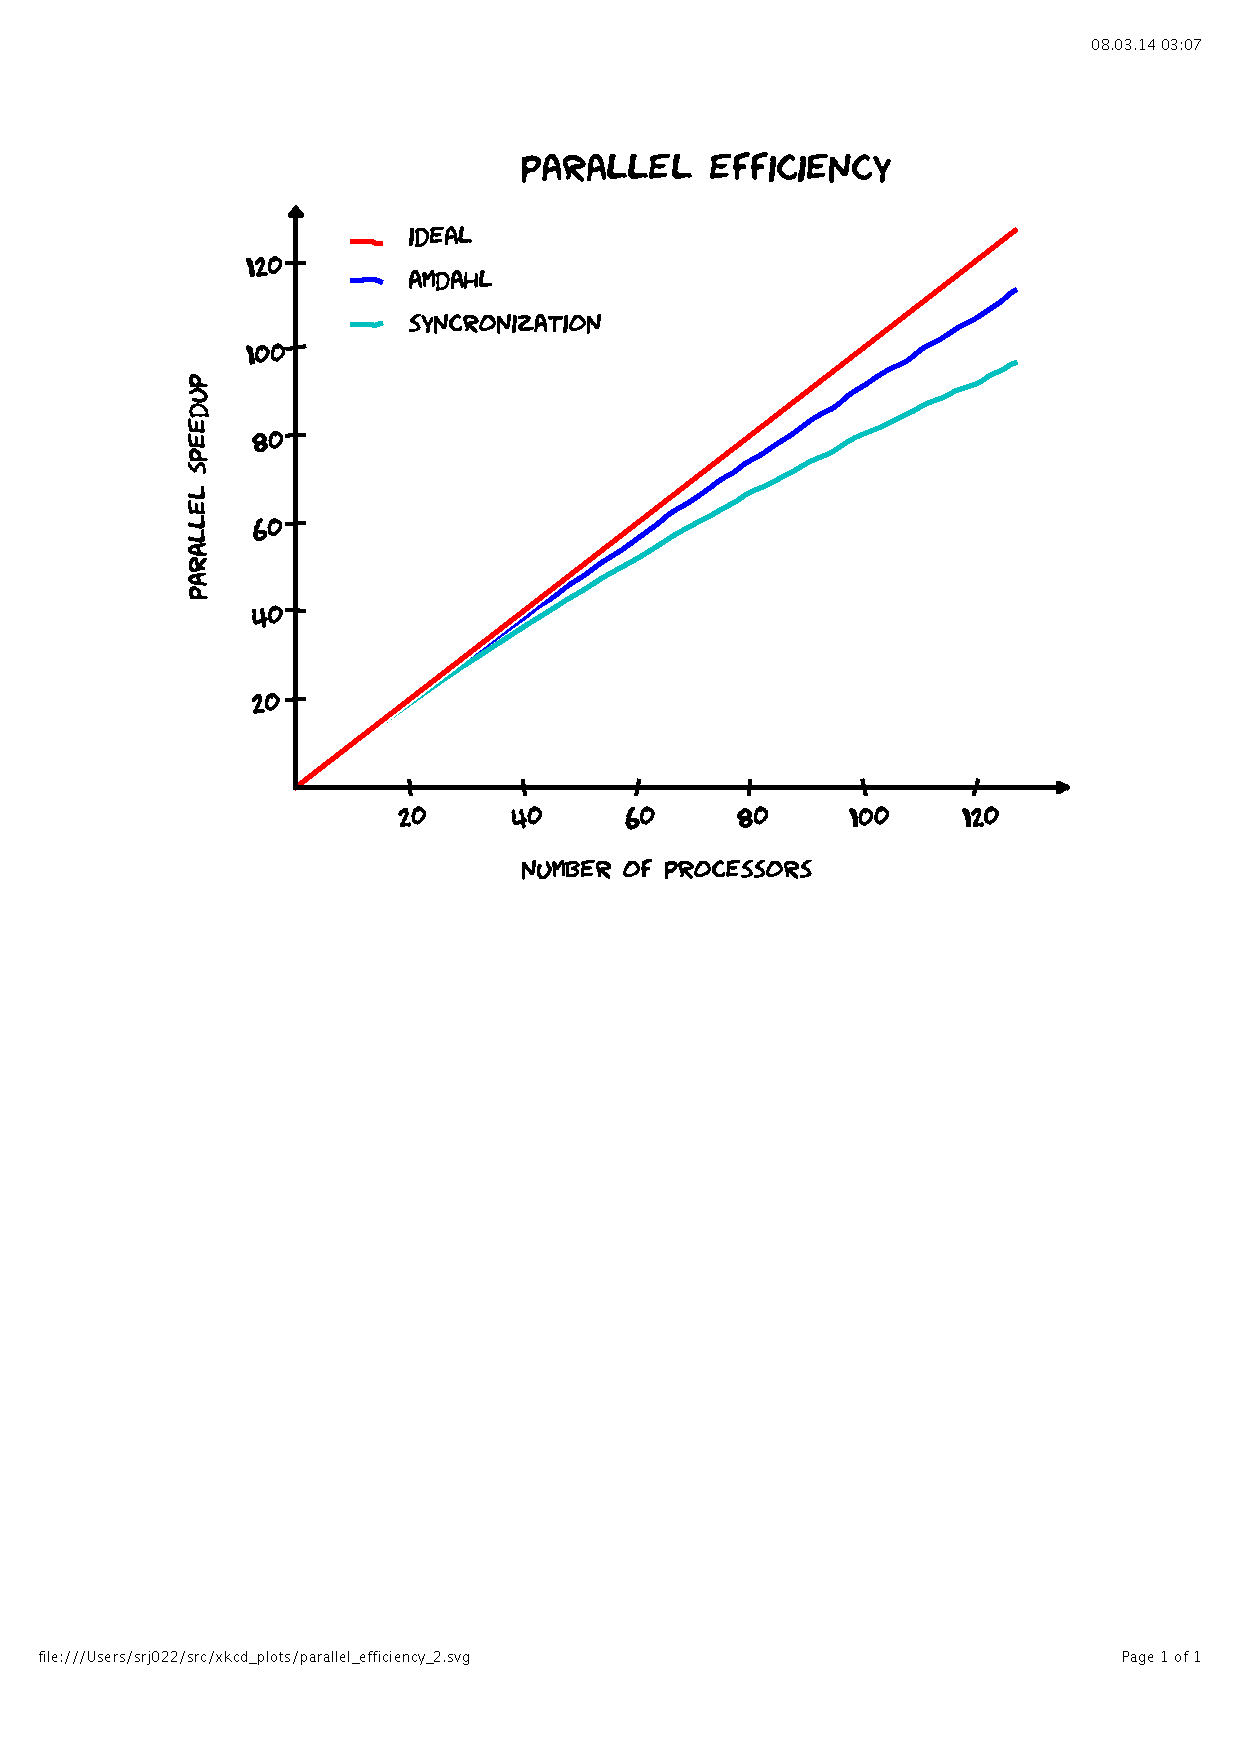
\includegraphics[clip, viewport = 50 250 550 800, scale=0.5]{figures/parallel_efficiency_2.pdf}}
    %\only<4>{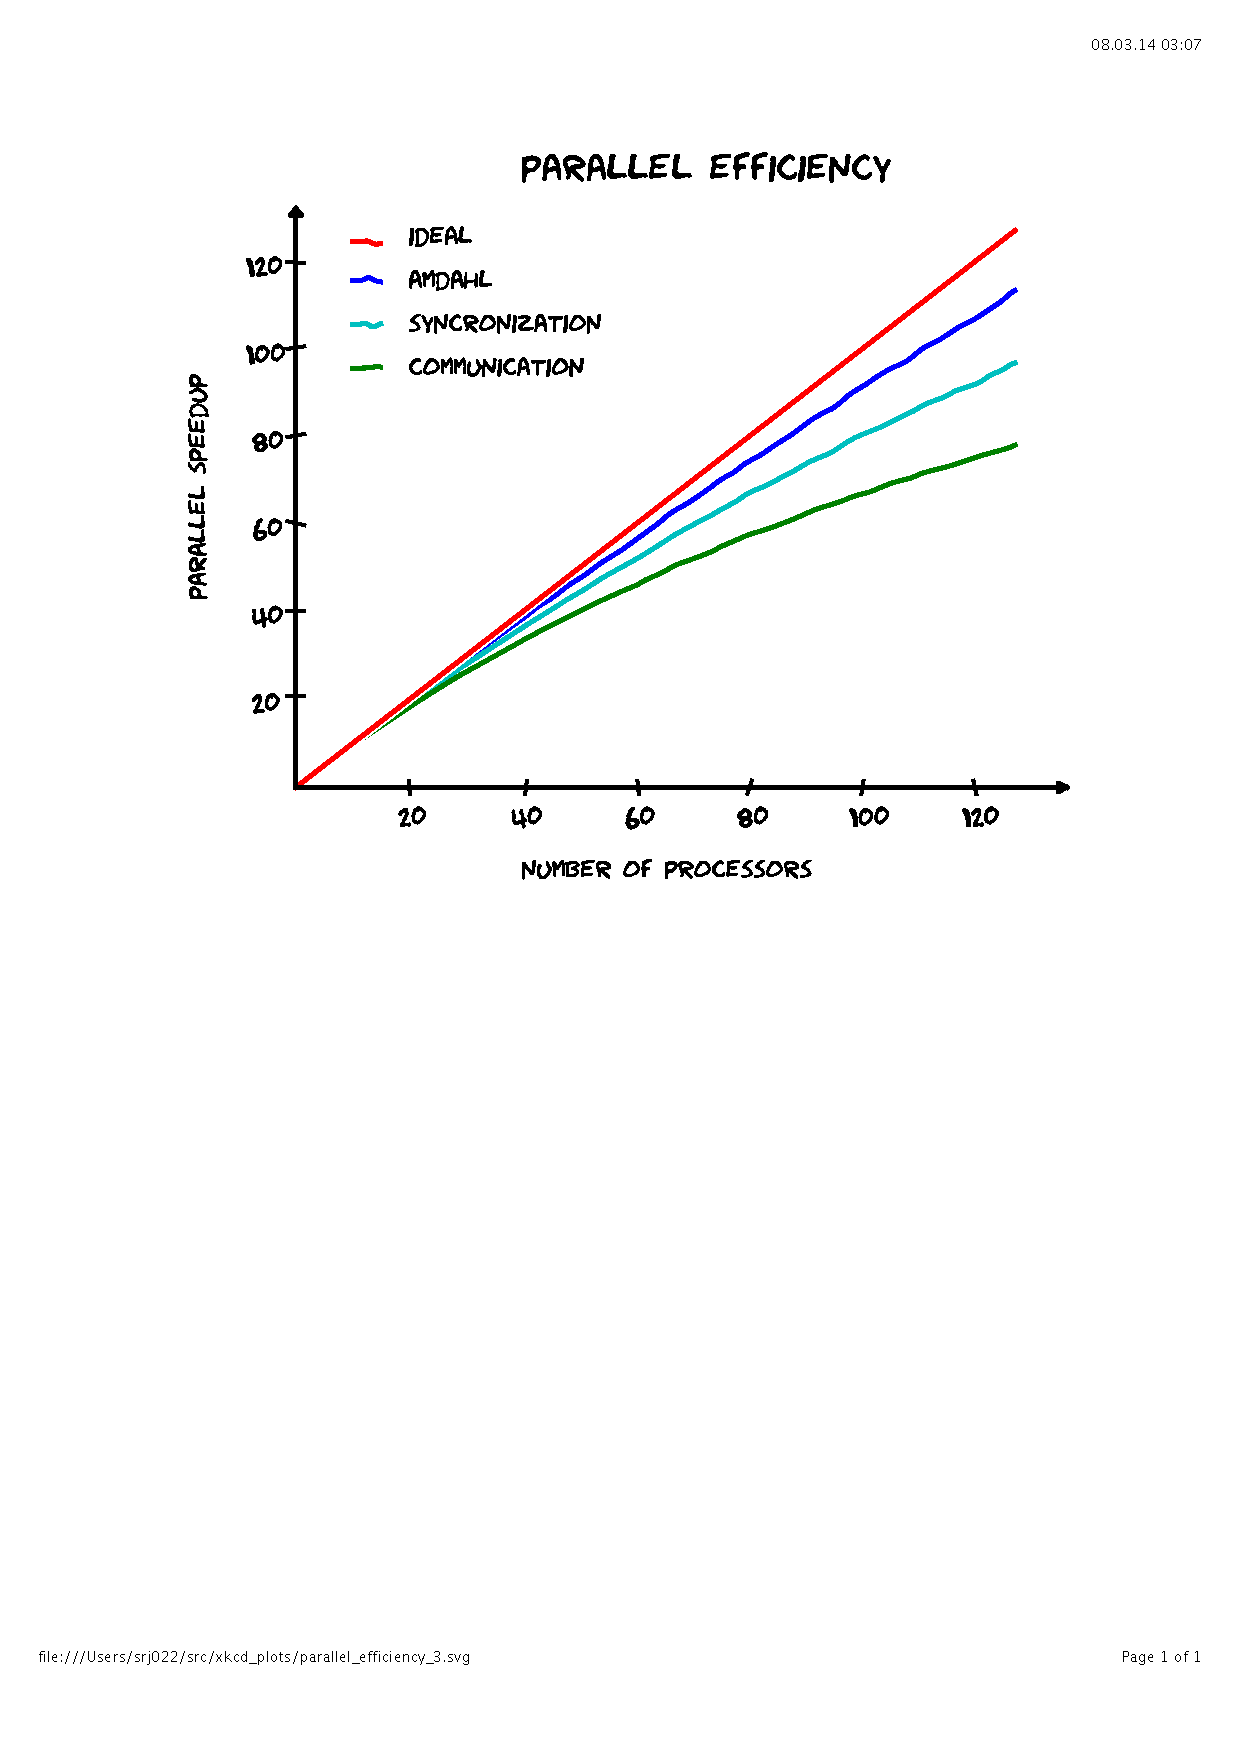
\includegraphics[clip, viewport = 50 250 550 800, scale=0.5]{figures/parallel_efficiency_3.pdf}}
    %\end{center}
%\end{frame}

\begin{frame}
    \frametitle{Parallelization}
    \begin{columns}
    \begin{column}{.5\textwidth}
	\ \ \ \ \textbf{Shared memory using OpenMP}
	\begin{itemize}
	    \item All CPUs have access to the \textbf{full} grid
	    \item No communication needed
	    \item Small scale parallelization ($<50$ CPUs)
	    \item Work (grid cells) dynamically distributed
	\end{itemize}
    \end{column}
    \begin{column}{.5\textwidth}
	\ \ \ \ \textbf{Distributed memory using MPI}
	\begin{itemize}
	    \item Each CPU has access to a \textbf{local} part of the grid
	    \item Communication required
	    \item Large scale parallelization ($>1000$ CPUs)
	    \item Work (grid cells) distributed \it{a priori}
	\end{itemize}
    \end{column}
    \end{columns}
    \ \\
    \ \\
    \ \\
    \ \\
    \begin{columns}
    \begin{column}{0.4\textwidth}
	\centering
	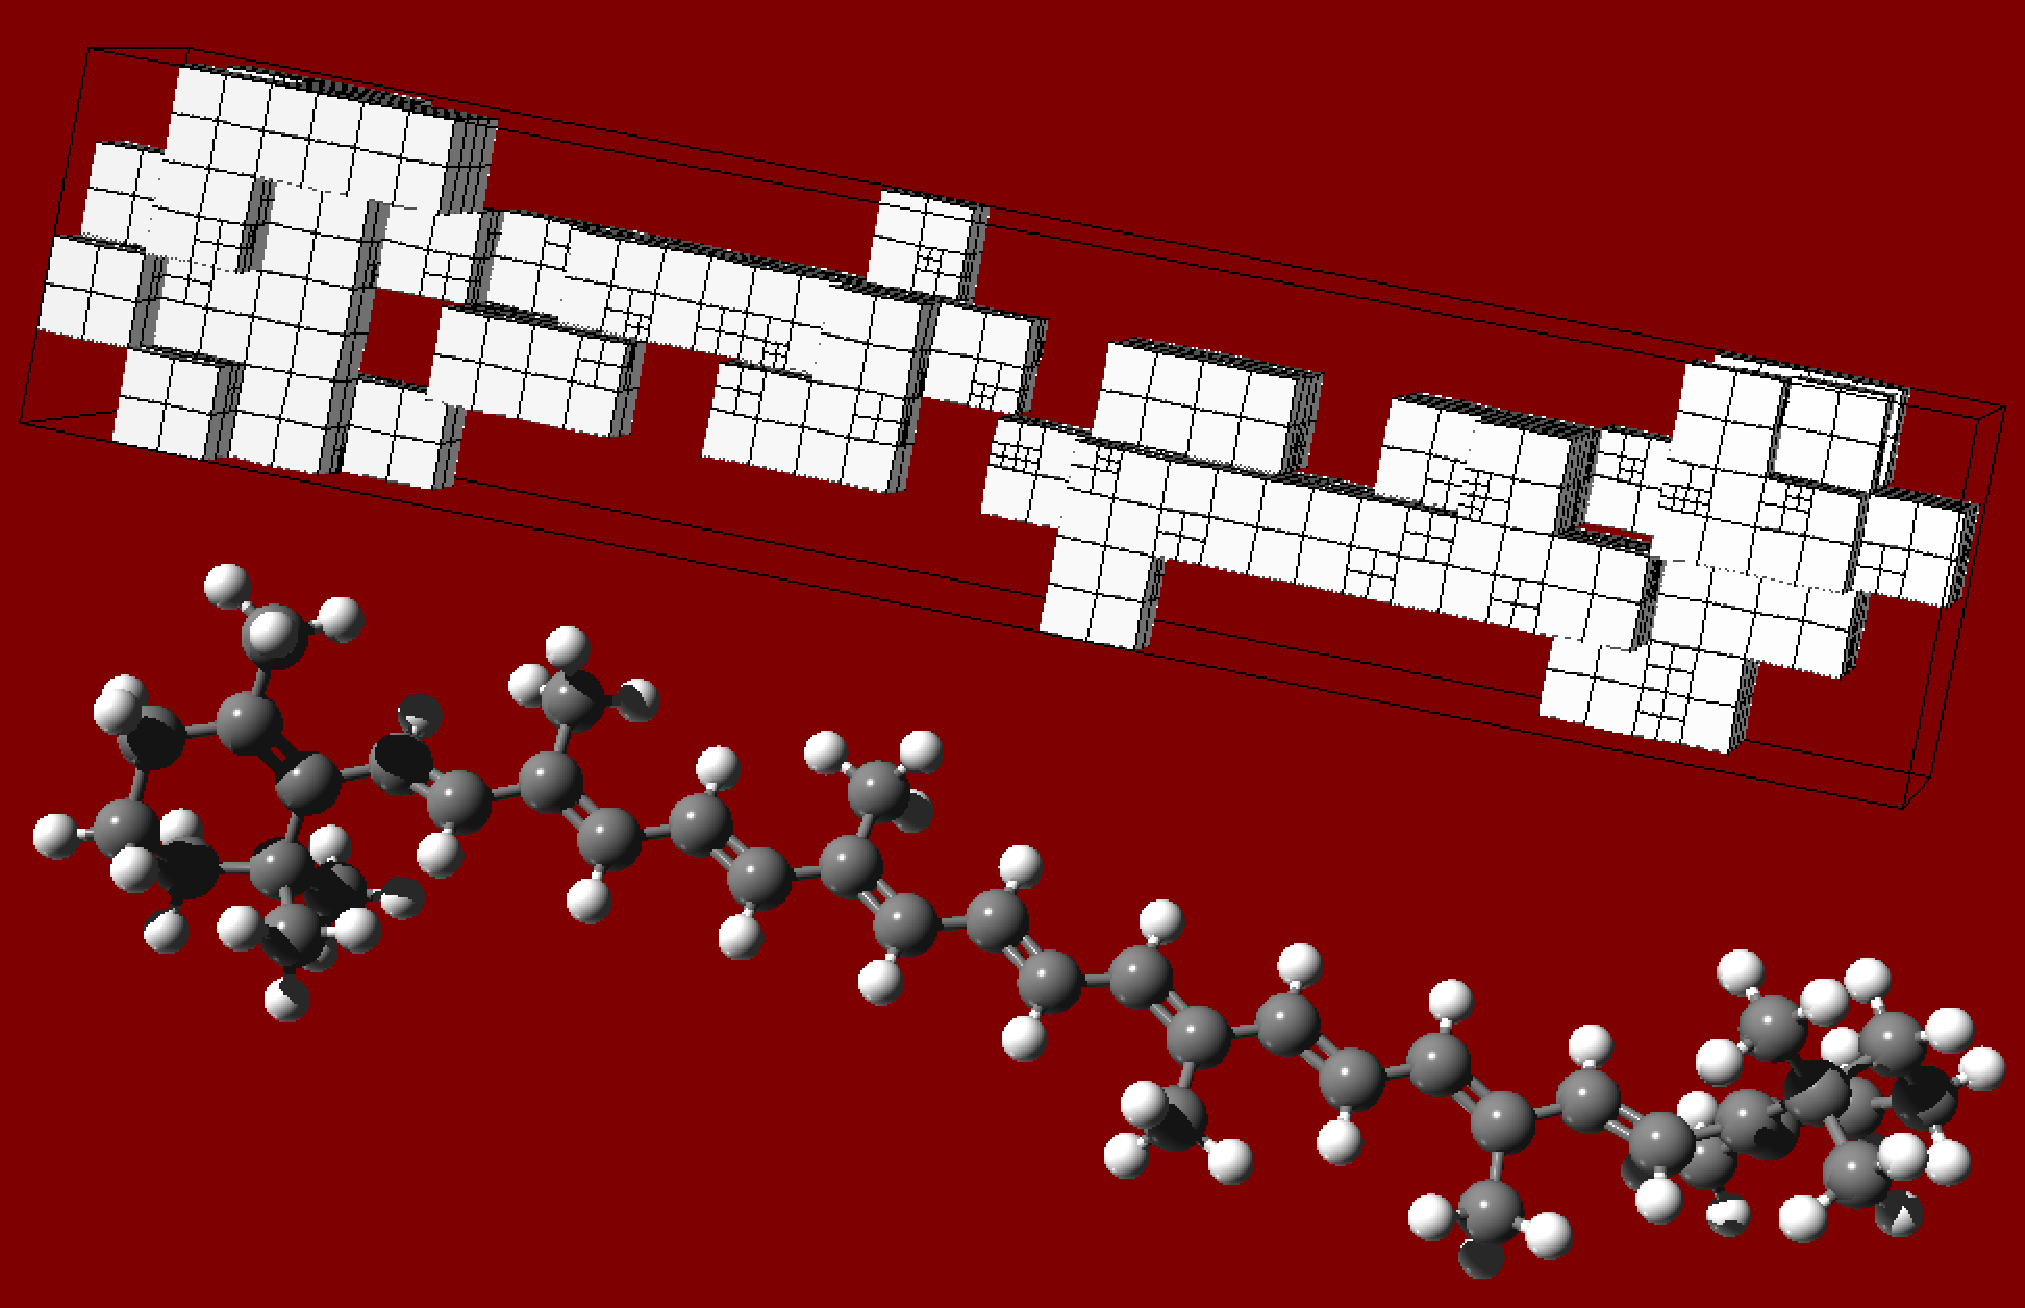
\includegraphics[angle=-90, scale=0.15]{figures/caroteneGrid.pdf}
    \end{column}
    \begin{column}{0.6\textwidth}
	\centering
	\textbf{Lebesgue path}
	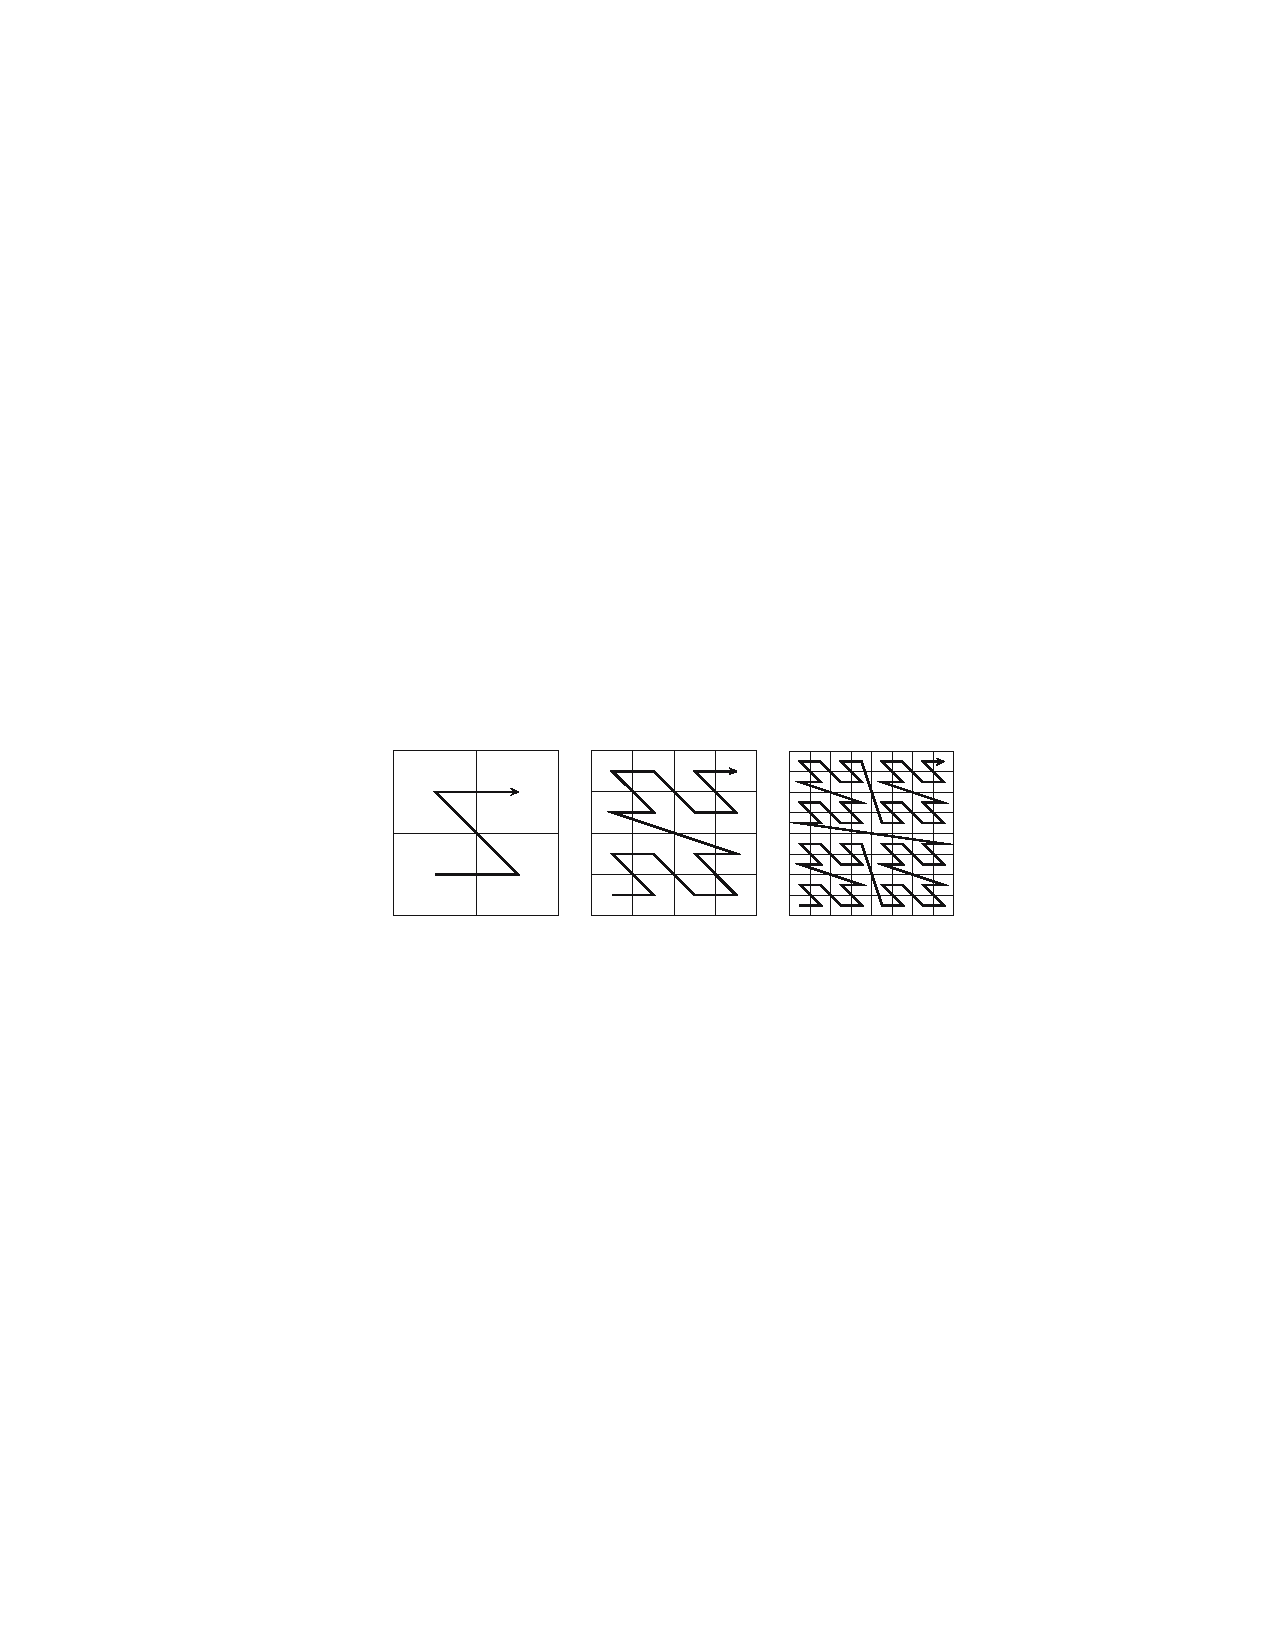
\includegraphics[scale=0.5, viewport = 150 350 500 435, clip]{figures/lebesgue.pdf}
	\ \\
	\ \\
	\ \\
	\textbf{Hilbert path}
	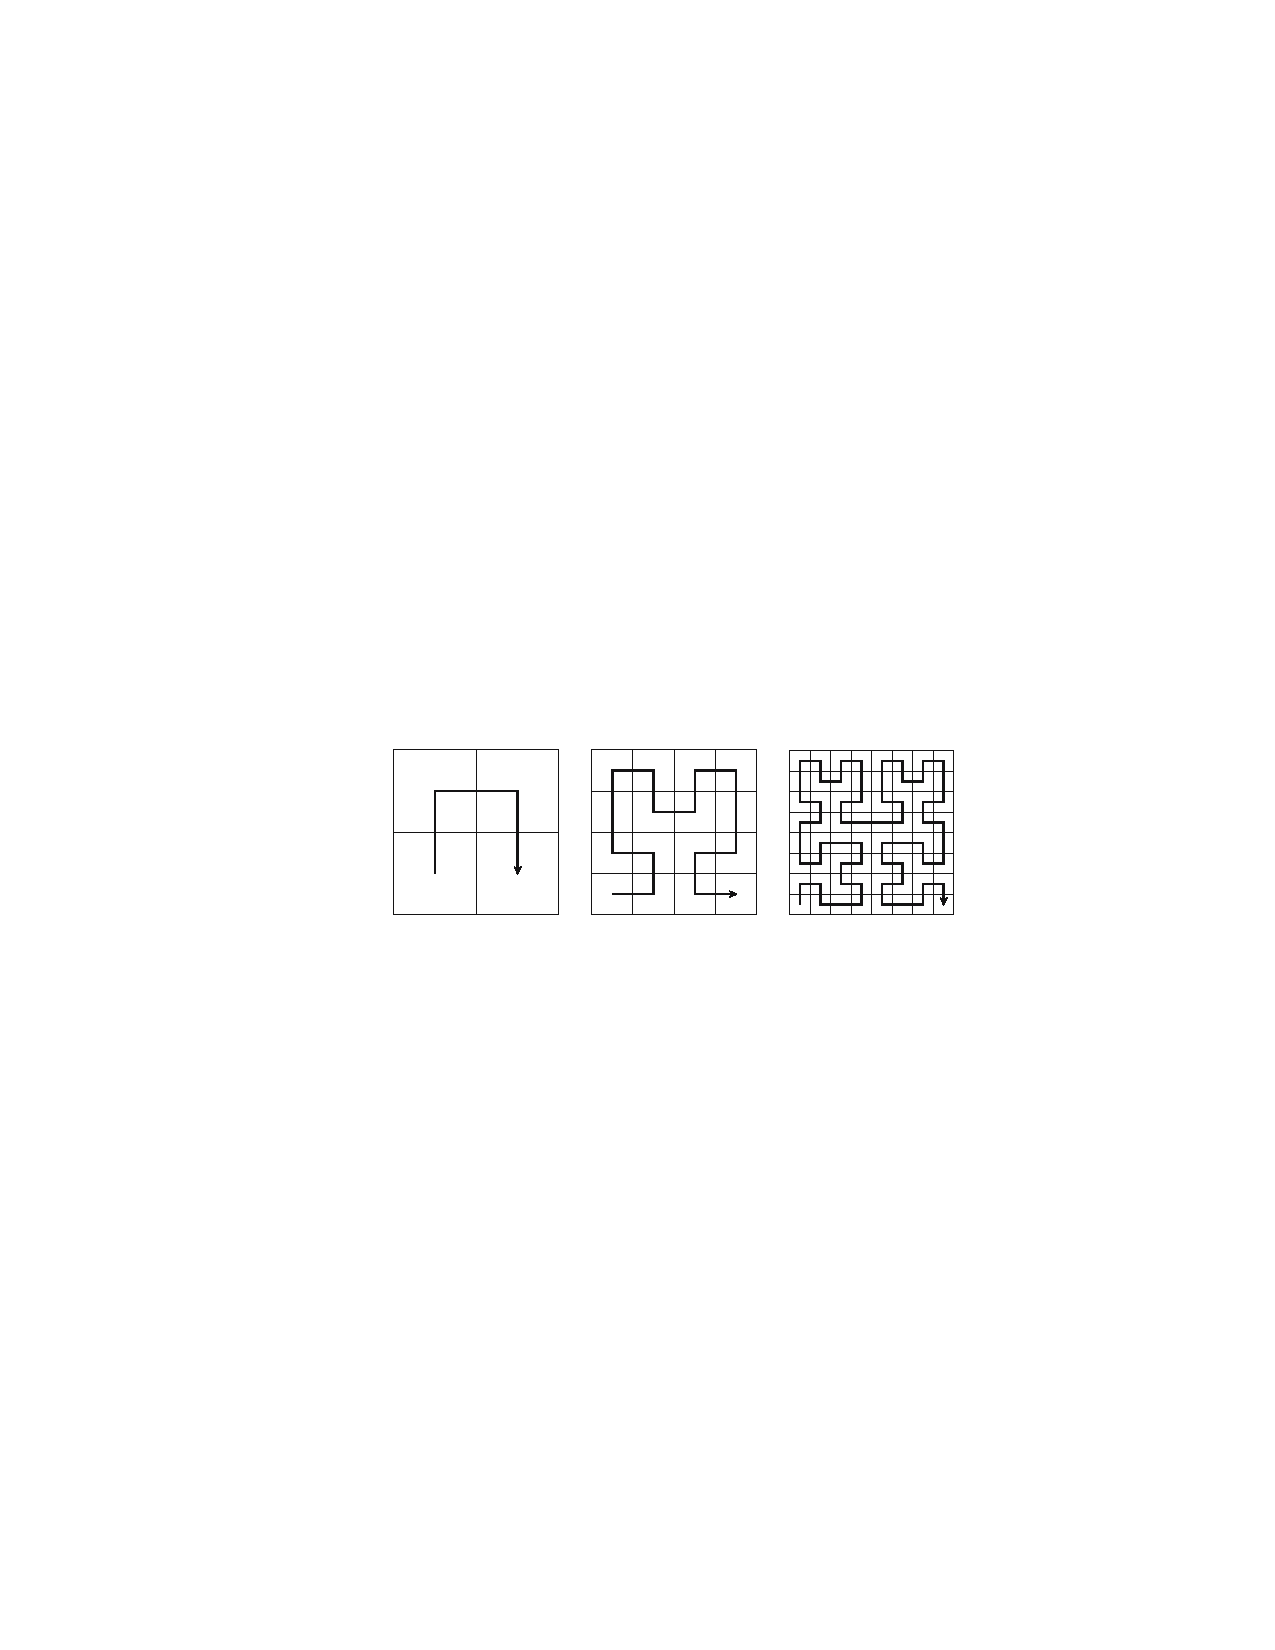
\includegraphics[scale=0.5, viewport = 150 350 500 435, clip]{figures/hilbert.pdf}
    \end{column}
    \end{columns}
\end{frame}

\begin{frame}
    \frametitle{Parallel algorithm}
    \begin{algorithmic}[1]
	\STATE \red{MPI:} assume input \tree distributed among hosts through Hilbert path
	\STATE create \tree skeleton of empty \nodes for the output function
	\STATE \red{MPI:} distribute output \nodes among hosts through Hilbert path
	\STATE create list of \emph{all} output \nodes
	\WHILE{number of output \nodes in the current list $N>0$}
	    \STATE \red{OpenMP:} divide the list of output \nodes among available processors
	    \FOR{each output \node in the current list}
		\STATE fetch \red{\emph{local}} input \nodes within bandwidth of the \emph{full} operator
		\STATE compute scaling and wavelet coefficients of output \node
	    \ENDFOR
	    \STATE \red{MPI:} communicate the \nodes of the output function to the appropriate host
	    \FOR{each \red{\emph{local}} \node of the output function}
		\STATE remove \node from current list
		\IF{\node needs to be refined}
		    \STATE allocate children \nodes (\red{inherits MPI ownership from parent})
		    \STATE add children \nodes to the current list
		\ENDIF
	    \ENDFOR
	    \STATE \red{MPI:} collect list of \emph{all} output \nodes for the next iteration
	\ENDWHILE
    \end{algorithmic}
\end{frame}

\begin{frame}
    \frametitle{OpenMP performance}
    \begin{columns}
    \begin{column}{.10\textwidth}
    \ \\
    \end{column}
    \begin{column}{.45\textwidth}
    \centering
    Electrostatic potential calculated to a relative precision of $\epsilon=10^{-6}$
    for diamond fragments
    \begin{equation}
	\nonumber
	C_{(2n+3)(n+2)(n+1)/6}H_{2(n+2)(n+1)}
    \end{equation}
    \ \\
    \ \\
    \ \\
    \textbf{Fitted curve}
    \begin{equation}
	\nonumber
	t_{rel}(n) = 11.6 + 1.84n^{0.805}
    \end{equation}
    \end{column}
    \begin{column}{.50\textwidth}
	\begin{figure}
	    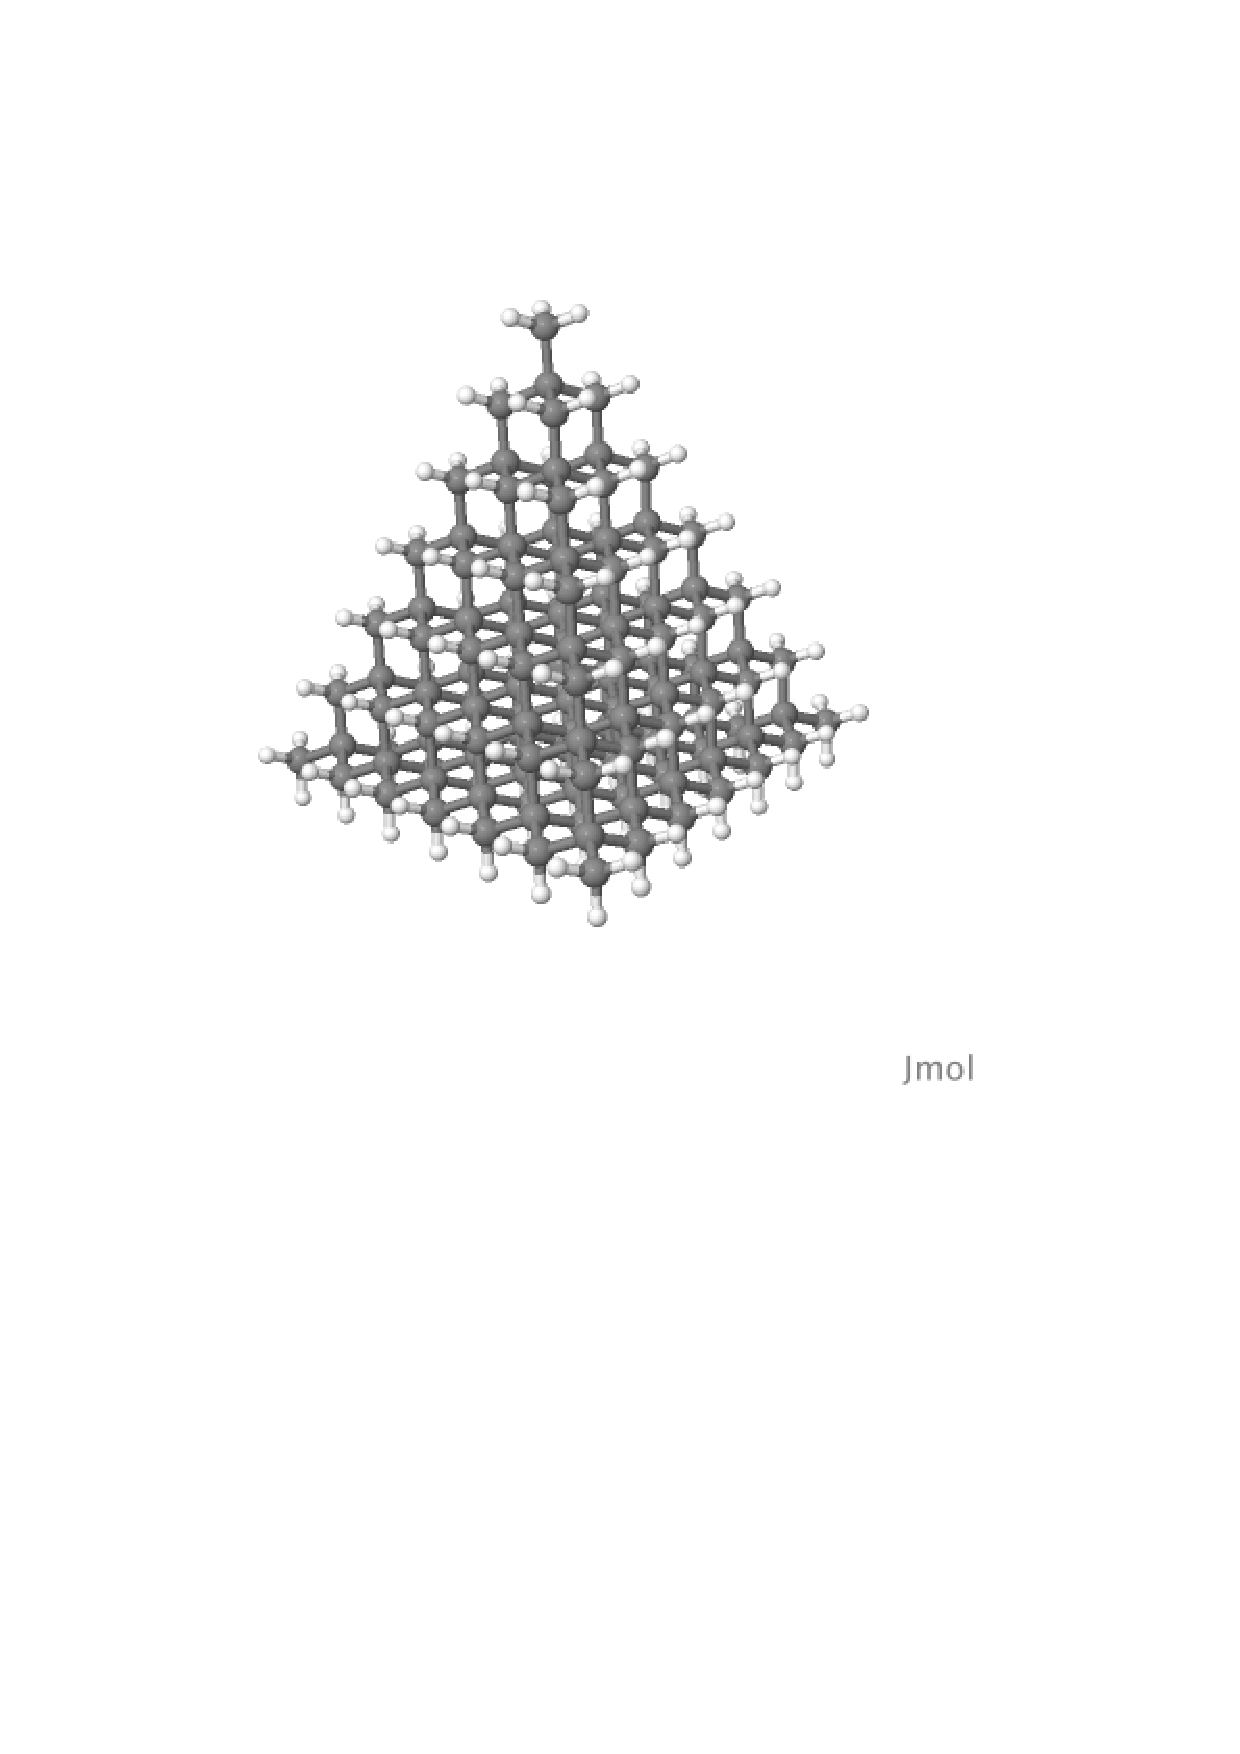
\includegraphics[scale=0.25, clip, viewport = 10 390 500 720]{figures/diamond.pdf}
	\end{figure}
    \end{column}
    \end{columns}    
    \begin{center}
	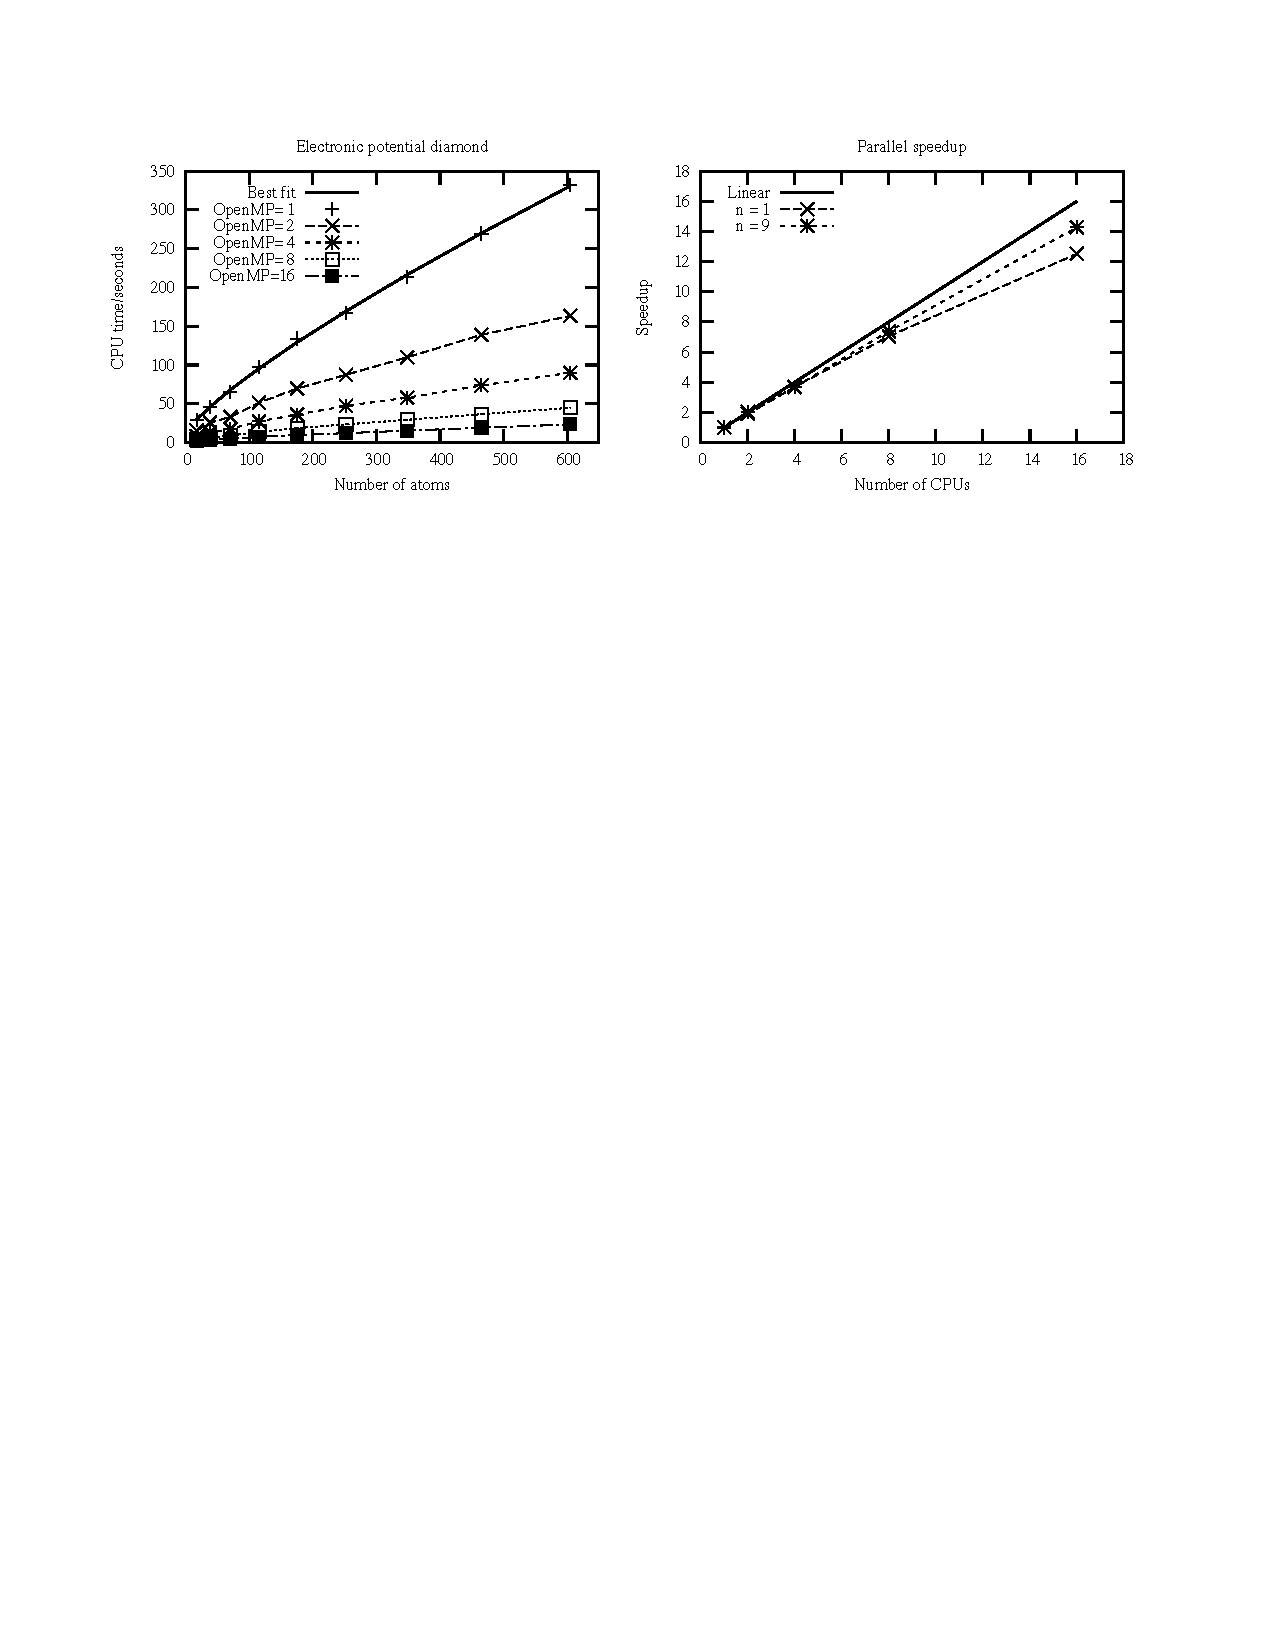
\includegraphics[scale=0.6, clip, viewport = 50 550 545 730]{figures/ompScaling.pdf}
    \end{center}
\end{frame}

\begin{frame}
    \frametitle{Hybrid MPI/OpenMP performance}
    \centering
    Wall clock computation time in seconds for parallel calculation of electronic potential\\
    of diamond fragments using pure OpenMP and hybrid MPI/OpenMP strategies.\\
    \begin{table}
    \tiny
    \begin{tabular}{cccrrrrrrrrr}
	\hline
	\hline                                                                           
	\multicolumn{3}{c}{Number of CPUs}&
	\multicolumn{9}{c}{Diamond system $n$ in $C_{(2n+3)(n+2)(n+1)/6}H_{2(n+2)(n+1)}$}\\
	MPI&OMP&TOT	&1	&2	&3	&4	&5	&6	&7	&8	&9	\\
	\hline
	   &   &   	&	&      	&	&	&	&	&	&	&	\\
	  1&  1&  1	& 29.4	& 46.2 	& 64.7 	& 97.8  &133.9  &166.8  &213.4  &269.4  &332.0  \\
	  1&  2&  2	& 15.5	& 25.5 	& 33.0 	& 51.3  & 69.5  & 87.2  &110.0  &138.9  &163.4  \\
	  1&  4&  4	&  8.0 	& 12.8 	& 17.4 	& 27.0  & 36.1  & 47.3  & 57.8  & 73.7  & 90.1  \\
	  1&  8&  8	&  4.2 	&  6.5 	&  8.8 	& 13.9  & 18.6  & 23.5  & 29.4  & 36.7  & 45.0  \\
	  1& 16& 16	&  2.4 	&  3.5 	&  4.7 	&  7.5  &  9.6  & 12.2  & 15.4  & 19.1  & 23.3  \\
	   %&   &   	&      	&      	&    	&    	&    	&	&	&	&	\\
	  %2&  1&  2	& 17.9 	& 28.4 	& 35.8 	& 59.2  & 81.6  & 93.0  &121.7  &147.5  &176.5  \\
	  %4&  1&  4	& 10.1 	& 16.3 	& 21.2 	& 32.5  & 51.6  & 53.8  & 60.8  & 85.3  &100.7  \\
	  %8&  1&  8	&  6.1 	&  9.4 	& 11.8 	& 19.9  & 25.6  & 28.0  & 35.4  & 43.7  & 50.7  \\
	 %16&  1& 16	&  5.0 	&  6.2 	&  8.2 	& 12.4  & 15.0  & 17.3  & 23.0  & 26.1  & 31.3  \\
	 %32&  1& 32	&  3.6 	&  4.2 	&  5.4 	&  9.5  &  9.2  & 10.9  & 14.1  & 16.8  & 20.0  \\
	 %64&  1& 64	&  3.1 	&  3.9 	&  4.3 	&  6.5  &  6.6  &  7.4  & 10.3  & 11.4  & 13.4  \\
	%128&  1&128	&  5.2 	&  5.7 	&  6.4 	&  7.6  &  7.8  &  8.8  & 10.9  & 10.9  & 11.9  \\
	   %&   &   	&      	&      	&      	& 	& 	& 	& 	& 	&	\\
	  2& 16& 32	&  1.5 	&  2.2 	&  2.9 	&  4.8  &  6.0  &  7.0  &  9.6  & 11.4  & 13.7  \\
	  4& 16& 64	&  1.1 	&  1.6 	&  2.0 	&  3.2  &  4.3  &  4.7  &  6.3  &  7.3  &  7.9  \\
	  8& 16&128	&  1.0 	&  1.4 	&  1.8 	&  2.9  &  3.3  &  3.8  &  4.8  &  5.9  &  6.4  \\
	 16& 16&256	&  0.9 	&  1.3 	&  1.6 	&  2.2  &  2.9  &  3.3  &  4.2  &  4.9  &  6.0  \\
	 32& 16&512	&  1.1 	&  1.3 	&  1.5 	&  2.0  &  2.4  &  2.8  &  3.4  &  4.0  &  4.8  \\
	   &   &   	&      	&      	&      	&    	&    	&	&	&	&	\\
	\hline                                                                           
	\hline
    \end{tabular}
    \end{table}
    \ \\
    \ \\
    \begin{itemize}
	\item Computation time can be pushed down to a few seconds for all systems
	\item Efficient OpenMP implementation (90\% at 16 CPUs)
	\item Hybrid MPI/OpenMP preferred over pure MPI for a given number of CPUs
    \end{itemize}
\end{frame}

%\begin{frame}
    %\centering
    %\Large{Part III:}\\
    %\ \\
    %\ \\
    %\centering
    %\Large{Real-space Density Functional Theory with\\ Localized Orbitals and Multiwavelets}
%\end{frame}

%\begin{frame}
    %\frametitle{The molecular Schr\"{o}dinger equation}
    %\ \\
    %\begin{equation}
	%\nonumber
	%\hat{H}\psi = E\psi
    %\end{equation}
    %\ \\
    %\begin{equation}
	%\nonumber
	%\hat{H} =   -\sum_I \frac{\nabla^2}{2M_I} - \sum_i \frac{\nabla^2}{2}
		    %%+\sum_{I>J} \frac{Z_IZ_J}{|\boldsymbol{R}_I-\boldsymbol{R}_J|} 
		    %-\sum_{i,I} \frac{Z_I}{|\boldsymbol{r}_i-\boldsymbol{R}_I|} 
		    %+\sum_{i>j} \frac{1}{|\boldsymbol{r}_i-\boldsymbol{r}_j|} 
    %\end{equation}
    %\ \\
    %\ \\
    %\ \\
    %\centering
    %For an $N$-particle problem, the wave function is $3N$-dimensional
    %\begin{equation}
	%\nonumber
	%\psi = \psi(\boldsymbol{r}_1,\boldsymbol{r}_2,\dots,\boldsymbol{r}_N)
    %\end{equation}
    %\ \\
    %\ \\
    %\ \\
    %\pause
    %\centering
    %$\beta$-Carotene ($C_{40}H_{56}$) has 296 electrons and an 888-dimensional wave function!
    %\only<1>{
    %\begin{center}
    %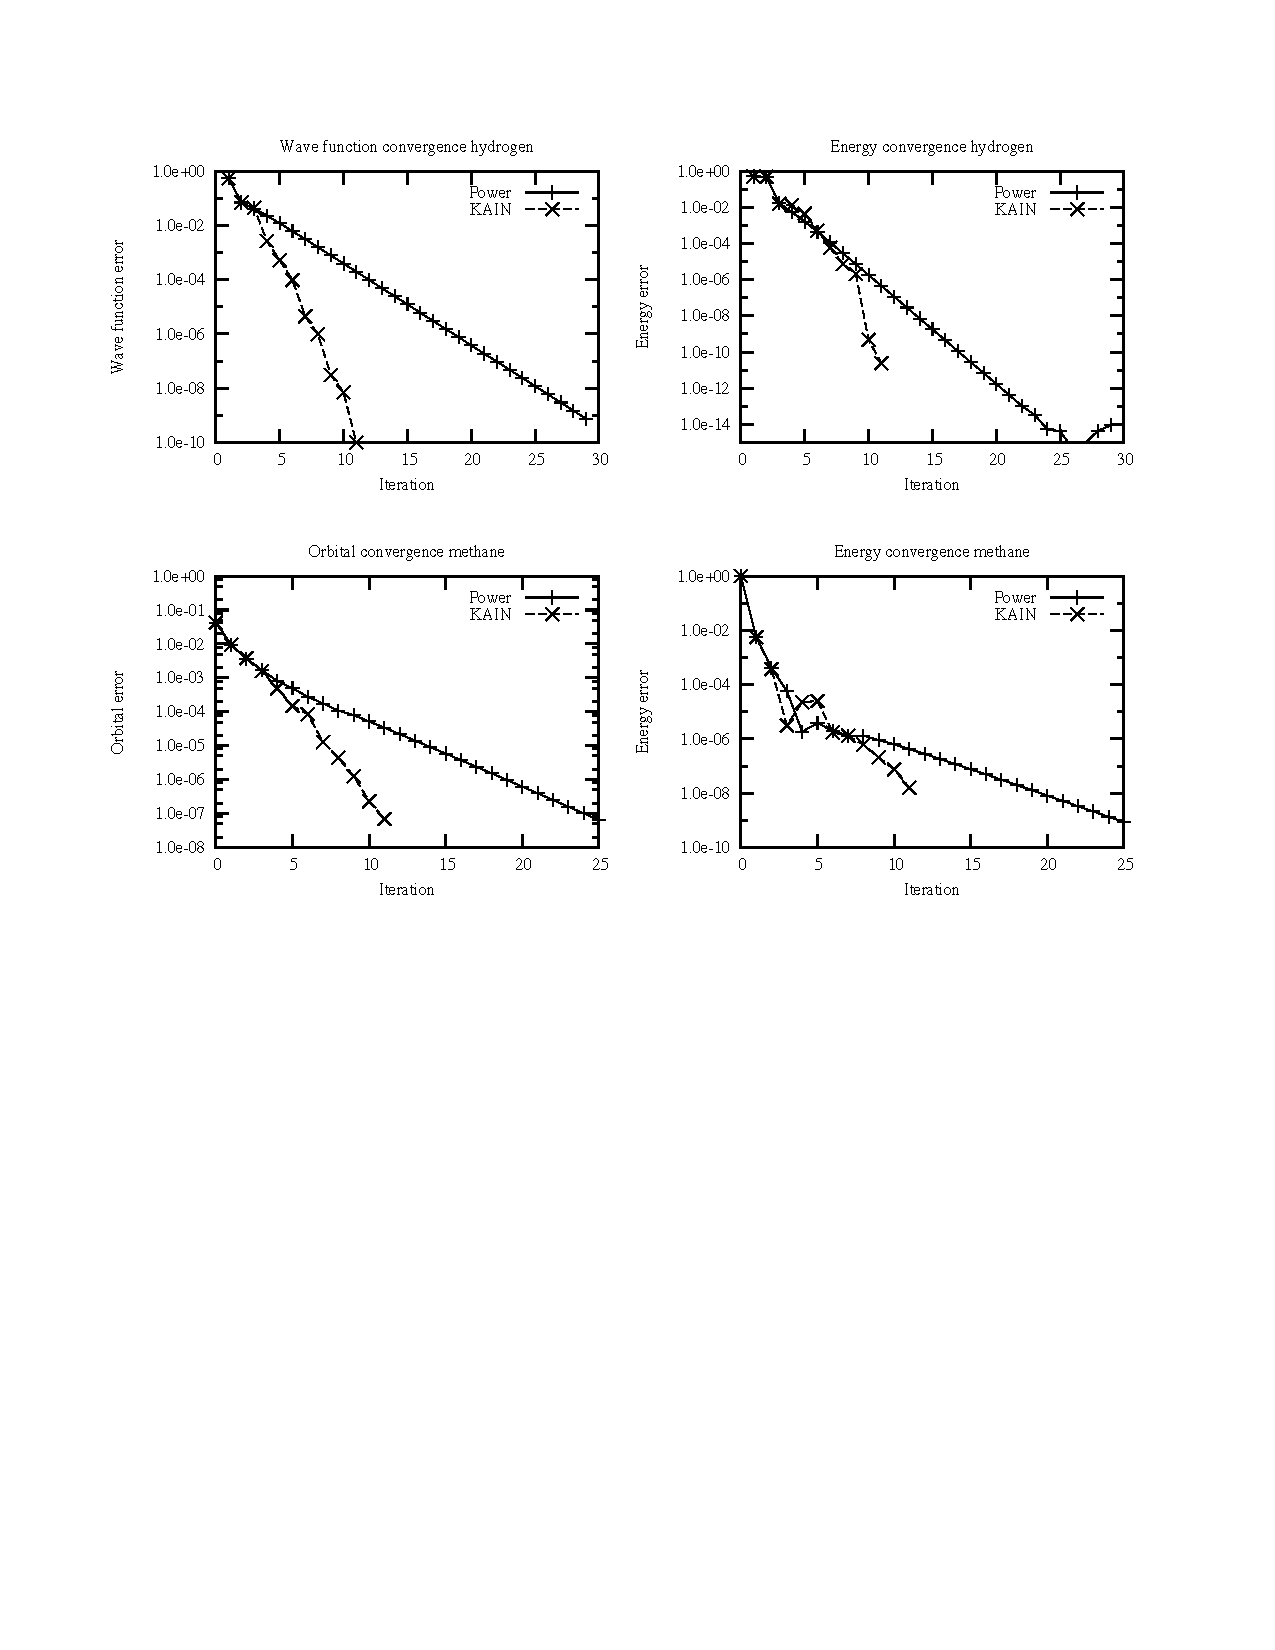
\includegraphics[scale=0.3, clip, viewport = 0 0 900 280]{figures/convergence.pdf}
    %\end{center}
    %}
    %\only<2>{
    %\begin{center}
    %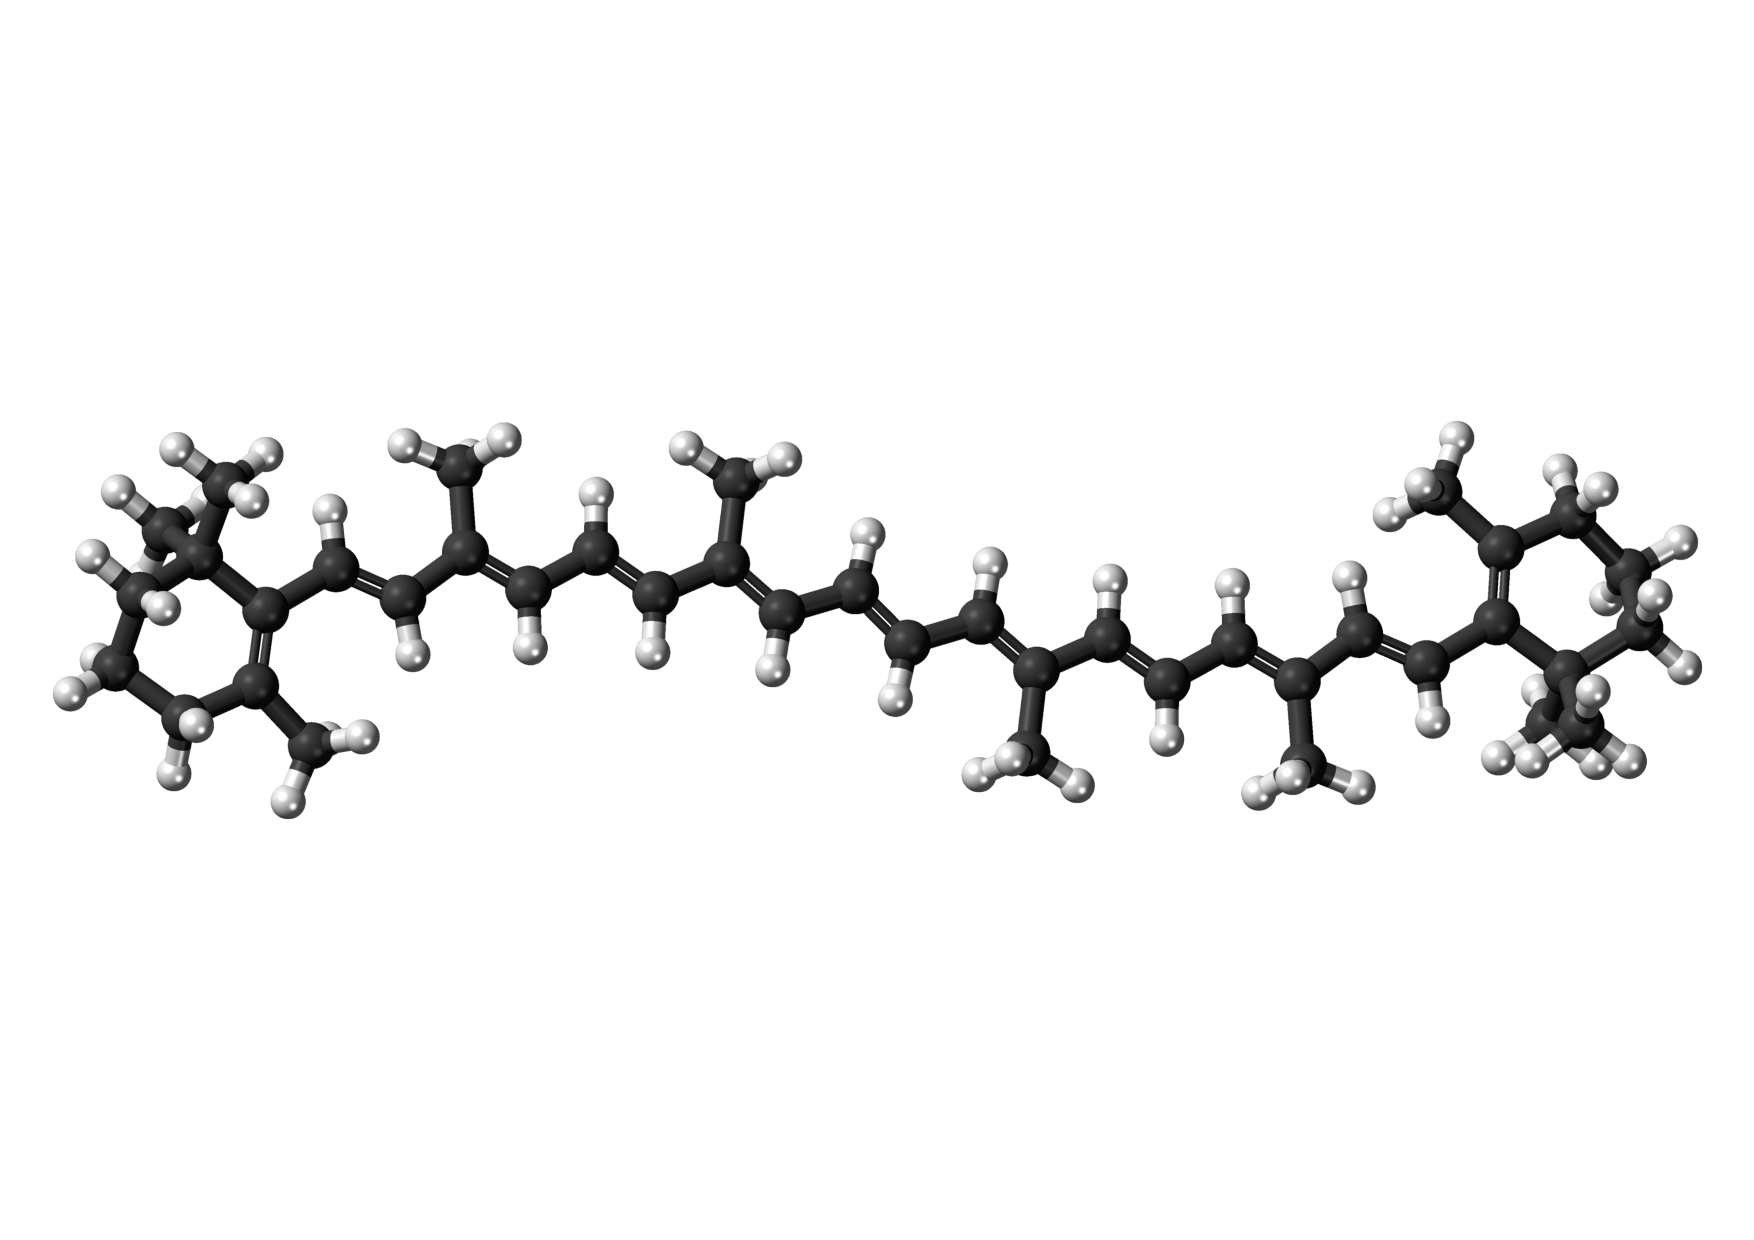
\includegraphics[scale=0.3, clip, viewport = 0 150 900 430]{figures/beta-carotene.pdf}
    %\end{center}
    %}
%\end{frame}

%\begin{frame}
    %\frametitle{Density Functional Theory}
    %\centering
    %Dramatically reduce the dimensionality
    %\begin{equation}
	%\nonumber
	%\rho(\boldsymbol{r}_1) = N \int |\psi(\boldsymbol{r}_1, \boldsymbol{r}_2,\dots,
	%\boldsymbol{r}_N)|^2 d\boldsymbol{r}_2\cdots d\boldsymbol{r}_N
    %\end{equation}
    %\ \\
    %\ \\
    %\ \\
    %\pause
    %Energy expressed as functional of the density
    %\begin{equation}
	%\nonumber
	%E[\rho] = T_s[\rho] + V_{ne}[\rho] + J[\rho] + E_{xc}[\rho]
    %\end{equation}
    %\ \\
    %\ \\
    %\ \\
    %\begin{columns}
    %\begin{column}{.50\textwidth}
    %\centering
    %\pause
    %\textbf{Energy expressions}
    %\begin{align}
	%\nonumber
	%V_{ne}[\rho]	&= \int \rho(\boldsymbol{r})v_{nuc}(\boldsymbol{r})d\boldsymbol{r}\\
	%\nonumber
			%&\\
	%\nonumber
	%J[\rho] &= \frac{1}{2} \int \rho(\boldsymbol{r})v_{el}(\boldsymbol{r})d\boldsymbol{r}\\
	%\nonumber
			%&\\
	%\nonumber
	%E_{xc}[\rho]	&= \int F_{xc}(\rho) d\boldsymbol{r}
    %\end{align}
    %\end{column}
    %\begin{column}{.50\textwidth}
    %\centering
    %\pause
    %\textbf{Potentials}
    %\begin{align}
	%\nonumber
	%v_{nuc}(\boldsymbol{r}) &= -\sum_I\frac{Z_I}{|\boldsymbol{r}-\boldsymbol{R}_I|}\\
	%\nonumber
			%&\\
	%\nonumber
	%v_{el}(\boldsymbol{r}) &= 
	    %\int \frac{\rho(\boldsymbol{r}')}{4\pi|\boldsymbol{r}-\boldsymbol{r}'|} d\boldsymbol{r}'\\
	%\nonumber
			%&\\
	%\nonumber
	%v_{xc}(\boldsymbol{r}) &= \frac{\delta E_{xc}[\rho]}{\delta\rho}
    %\end{align}
    %\end{column}
    %\end{columns}    
%\end{frame}
%
%\begin{frame}
    %\frametitle{Kohn-Sham DFT}
    %\centering
    %Express density through one-electron orbitals
    %\begin{equation}
	%\nonumber
	%\rho(\boldsymbol{r}) = \sum_i |\phi_i(\boldsymbol{r})|^2
    %\end{equation}
    %\ \\
    %\ \\
    %\ \\
    %\ \\
    %\pause
    %\begin{columns}
    %\begin{column}{.50\textwidth}
    %\centering
    %Kinetic energy
    %\begin{equation}
	%\nonumber
	%T_s[\rho] = -\sum_i \frac{1}{2}\nabla^2\phi_i(\boldsymbol{r})
    %\end{equation}
    %\end{column}
    %\begin{column}{.50\textwidth}
    %\centering
    %Effective potential
    %\begin{equation}
	%\nonumber
	%v_{eff}(\boldsymbol{r}) = v_{nuc}(\boldsymbol{r}) + v_{el}(\boldsymbol{r}) + v_{xc}(\boldsymbol{r})
    %\end{equation}
    %\end{column}
    %\end{columns}
    %\ \\
    %\ \\
    %\ \\
    %\ \\
    %\pause
    %\centering
    %\textbf{The Kohn-Sham equations}
    %\begin{equation}
	%\nonumber
	%\left[-\frac{1}{2}\nabla^2 + v_{eff}(\boldsymbol{r})\right]\phi_i(\boldsymbol{r}) = 
	%\epsilon_i\phi_i(\boldsymbol{r})
    %\end{equation}
%\end{frame}

%\begin{frame}
    %\frametitle{Computational chemistry}
    %\begin{center}
    %\only<1>{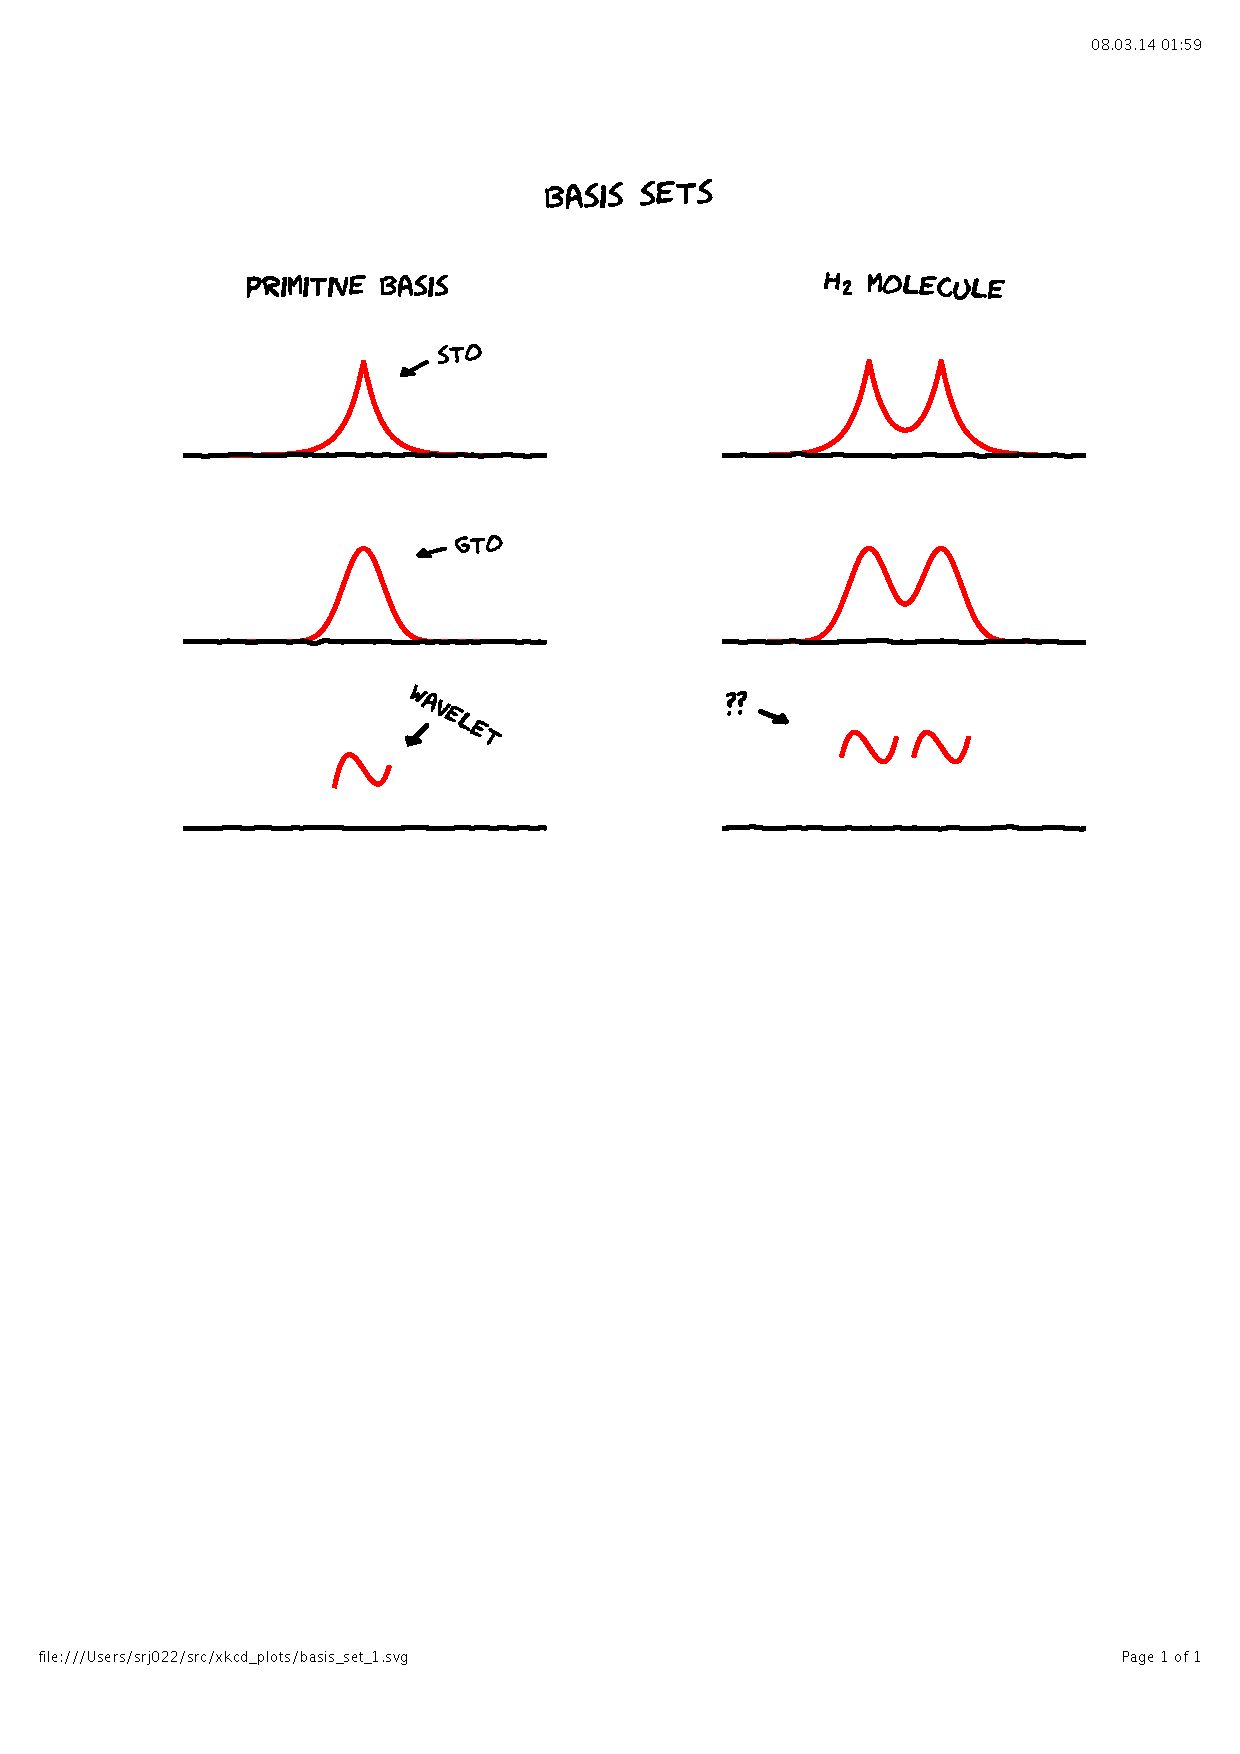
\includegraphics[scale=0.5, clip, viewport = 50 300 550 800]{figures/basis_set_1.pdf}}
    %\only<2>{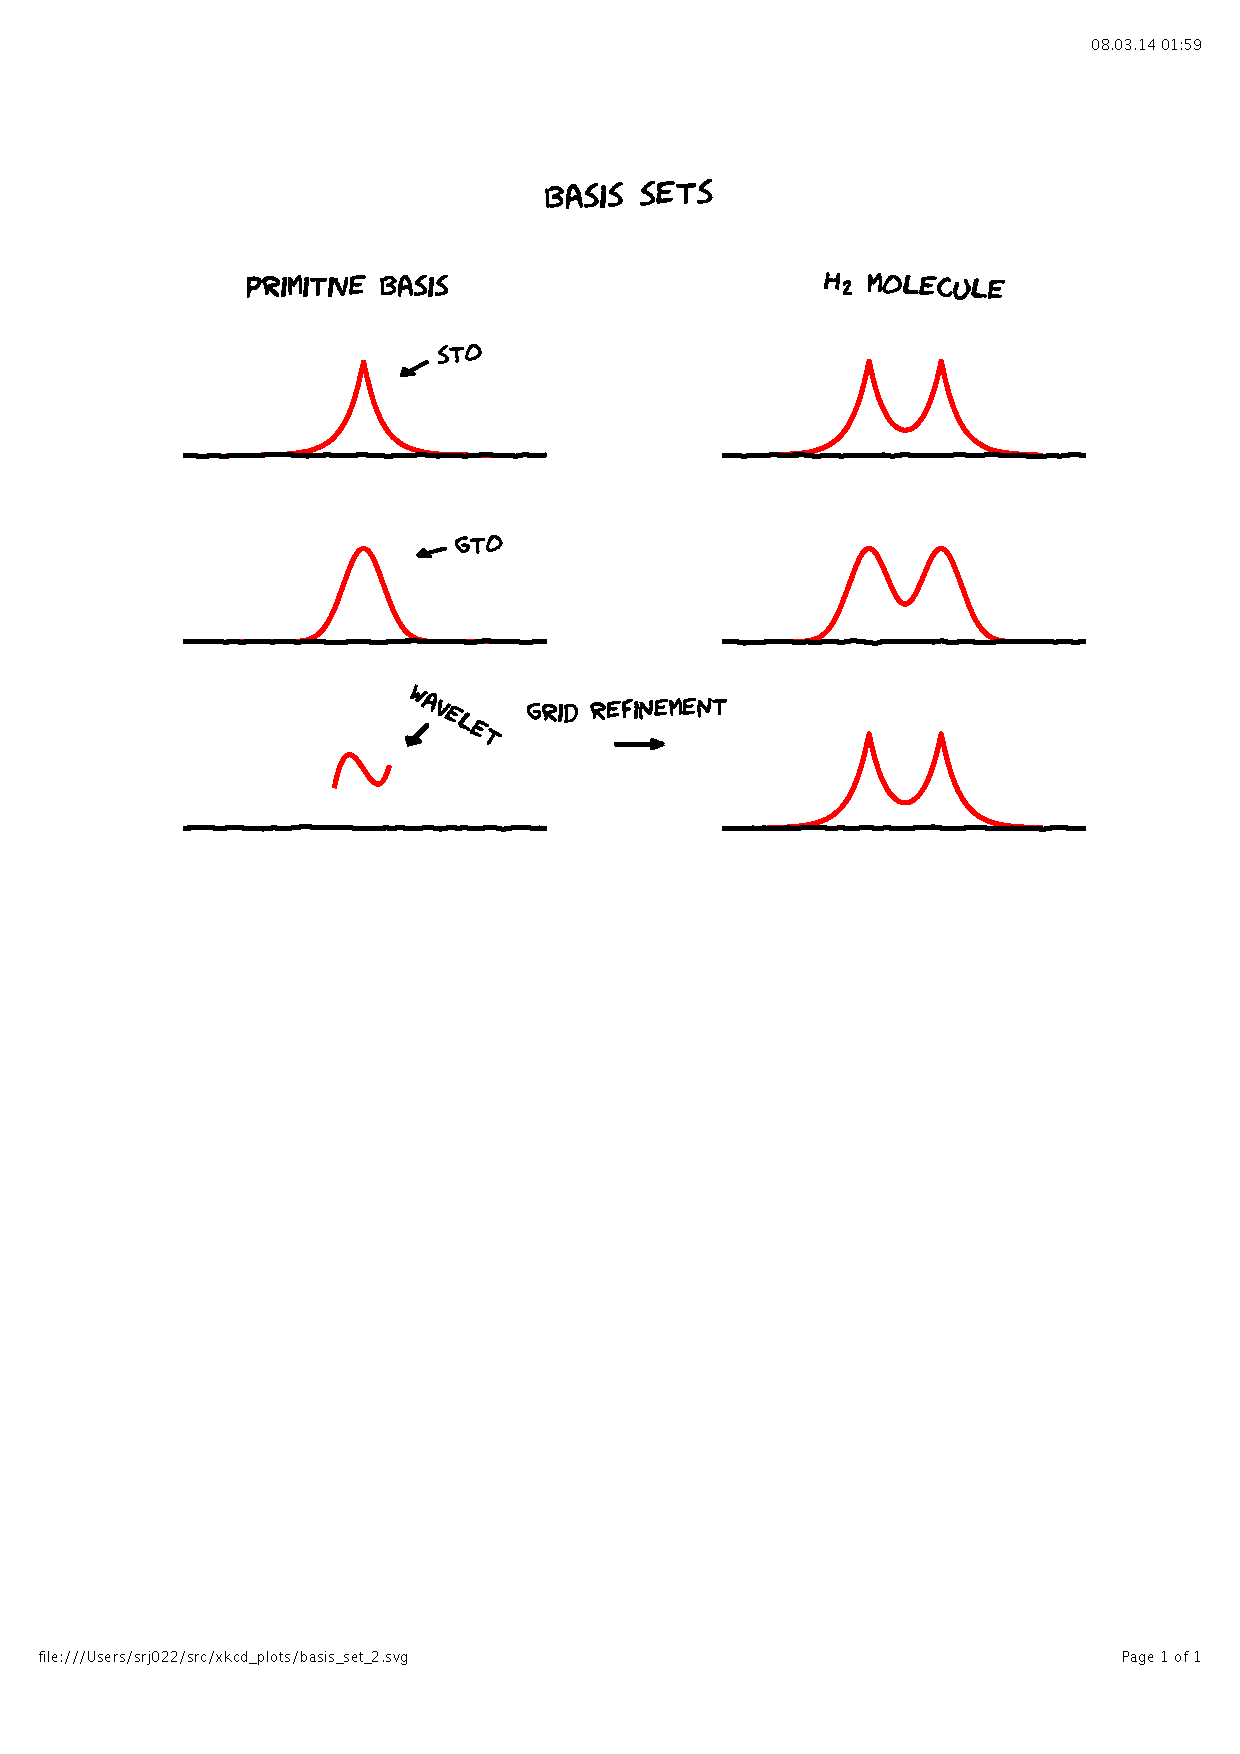
\includegraphics[scale=0.5, clip, viewport = 50 300 550 800]{figures/basis_set_2.pdf}}
    %\only<3>{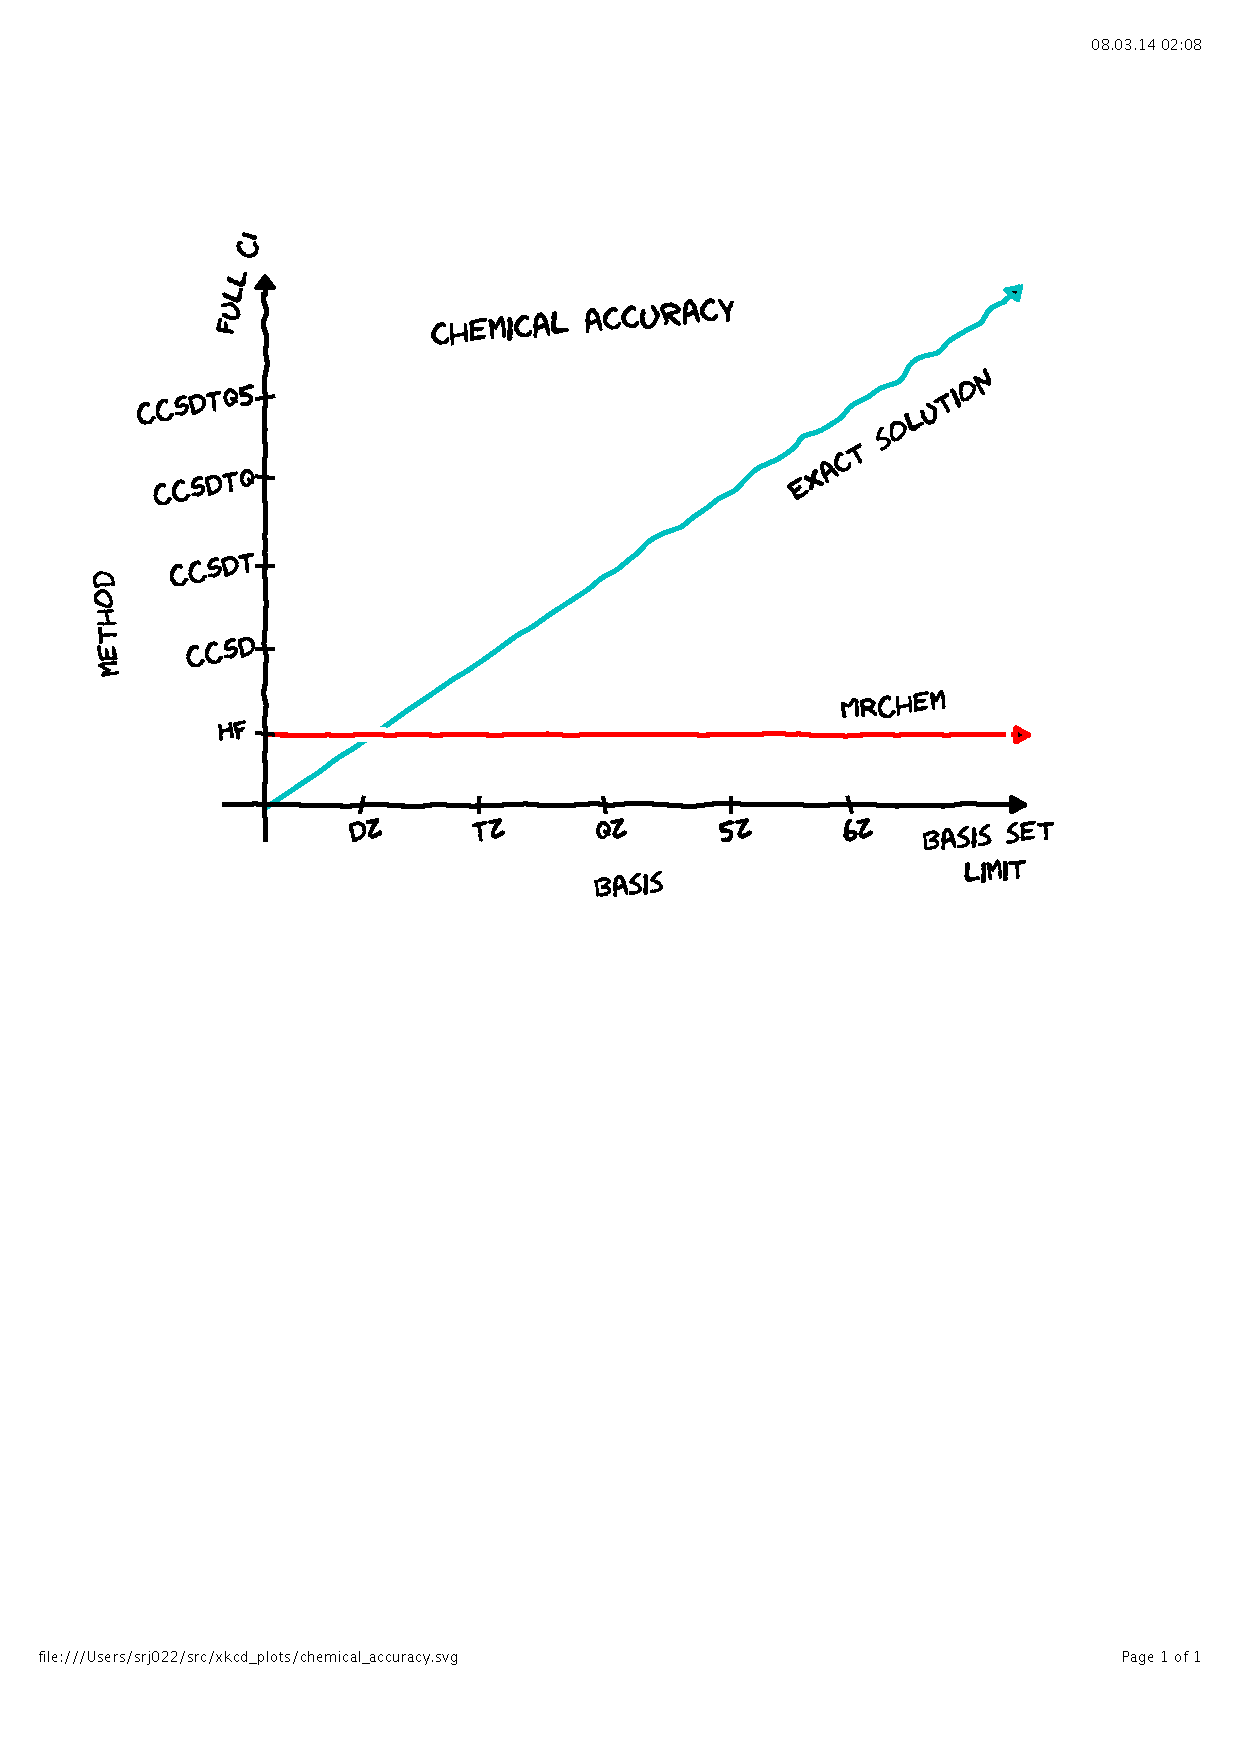
\includegraphics[scale=0.5, clip, viewport = 0 300 550 800]{figures/chemical_accuracy.pdf}}
    %\end{center}
%\end{frame}
%
%\begin{frame}
    %\frametitle{Integral formulation}
    %\centering
    %The Kohn-Sham equations
    %\begin{equation}
	%\nonumber
	%\left[-\frac{1}{2}\nabla^2 + v_{eff}(\boldsymbol{r})\right]
	%\phi_i(\boldsymbol{r}) =\ \epsilon_i \phi(\boldsymbol{r})
    %\end{equation}
    %\ \\
    %\ \\
    %\ \\
    %\ \\
    %\pause
    %can be expressed in integral form
    %\begin{equation}
	%\nonumber
	%\phi_i(\boldsymbol{r}) =\ -2\int H^{\mu}(\boldsymbol{r}-\boldsymbol{r}')\
	    %\Big[v_{eff}(\boldsymbol{r}') \phi_i(\boldsymbol{r}')\Big] d\boldsymbol{r}'
    %\end{equation}
    %\ \\
    %\ \\
    %\ \\
    %\ \\
    %\pause
    %and solved iteratively
    %\begin{equation}
	%\nonumber
	%\phi_i^{n+1} =\ -2\hat{H}\left[v_{eff}^n\phi_i^n\right]
    %\end{equation}
    %\ \\
    %\ \\
    %\ \\
    %\ \\
    %standard iterative subspace acceleration techniques (KAIN or DIIS) can be applied
%\end{frame}
%
%\begin{frame}
    %\frametitle{Hydrogen atom}
    %\centering
    %\textbf{Power iteration}
    %\begin{equation}
	%\nonumber
	%\phi^{n+1} = -2\hat{H}\left[v_{nuc}\phi^n\right]
    %\end{equation}
    %\ \\
    %\ \\
    %\ \\
    %\begin{columns}
    %\begin{column}{.10\textwidth}
    %\ \\
    %\end{column}
    %\begin{column}{.40\textwidth}
    %\centering
    %\textbf{Orbital update}
    %\begin{equation}
	%\nonumber
	%\Delta\phi^n = \phi^{n+1} - \phi^n
    %\end{equation}
    %\end{column}
    %\begin{column}{.50\textwidth}
    %\centering
    %\textbf{Energy update}
    %\begin{equation}
	%\nonumber
	%\Delta \epsilon^n = \left<\phi^{n+1}|v_{nuc}|\Delta\phi^n\right>
    %\end{equation}
    %\end{column}
    %\end{columns}    
    %\begin{center}
	%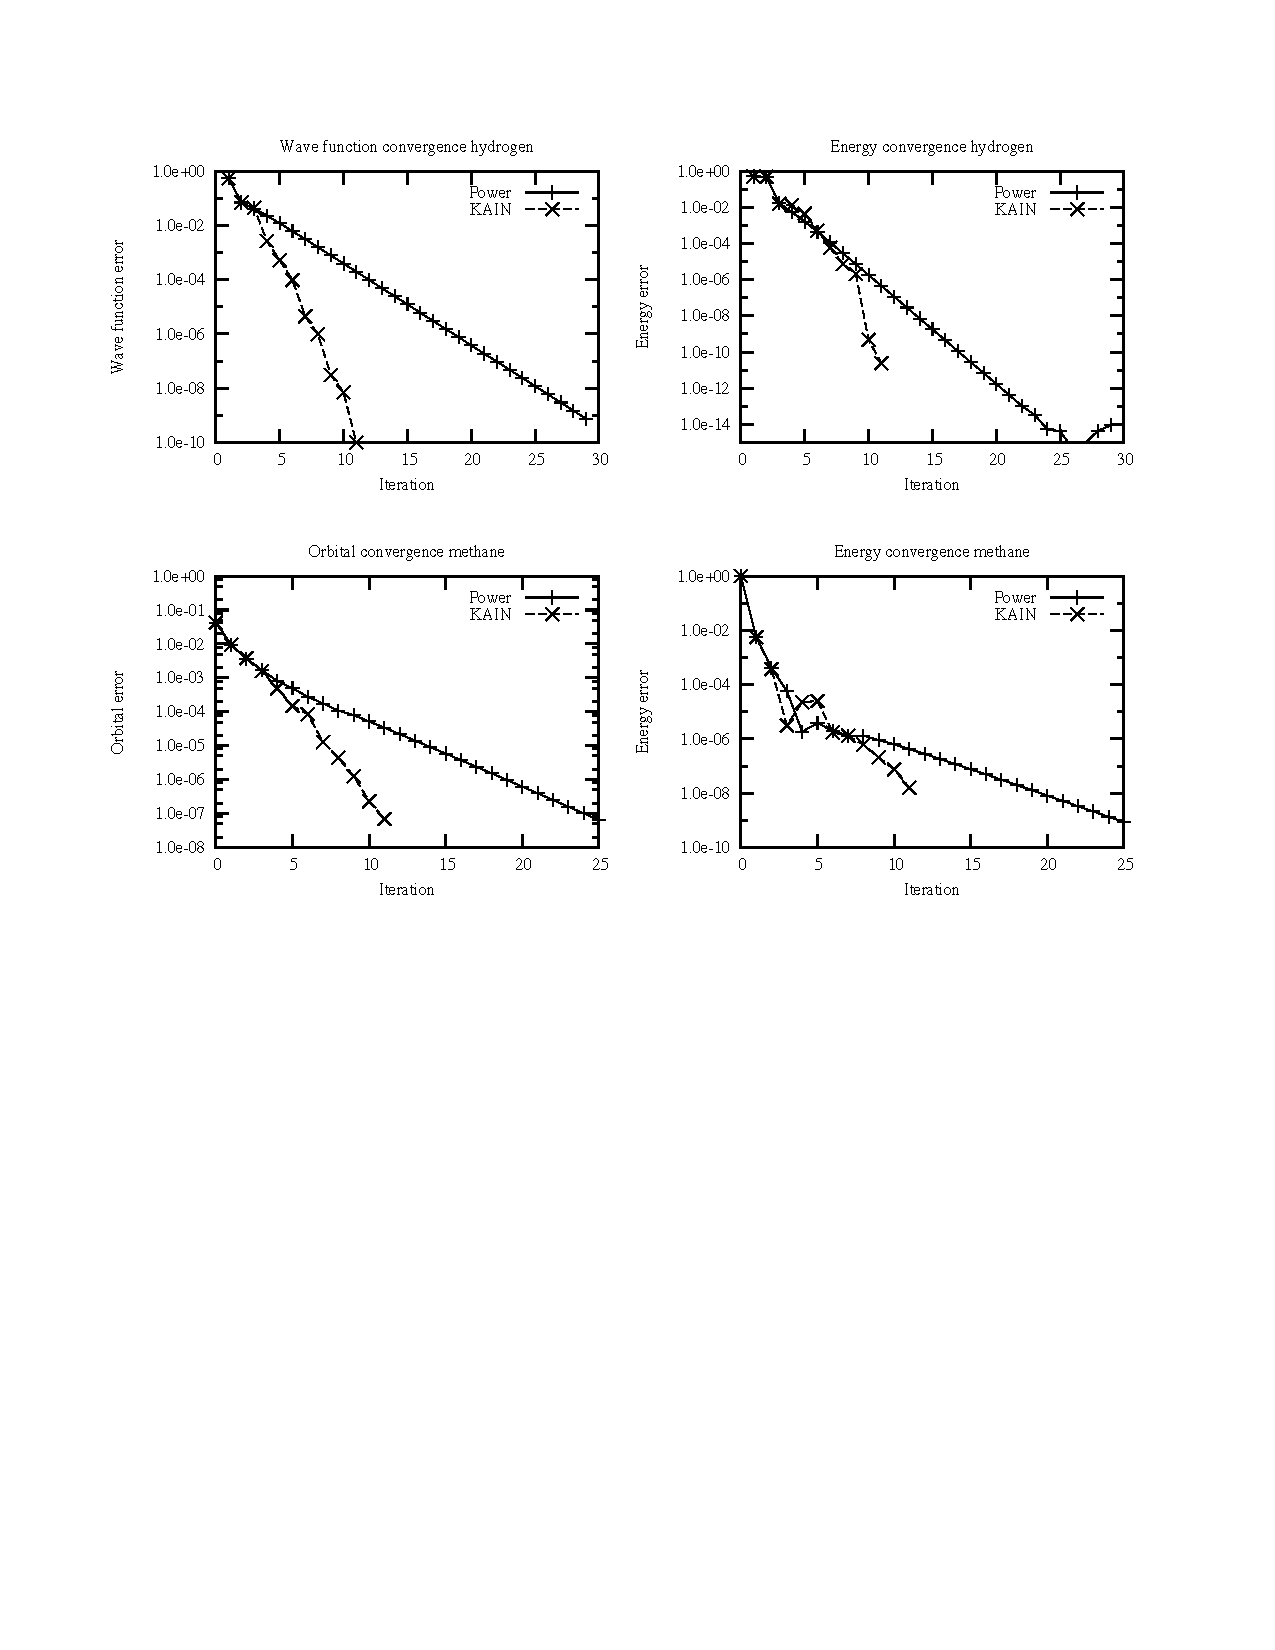
\includegraphics[scale=0.6, clip, viewport = 50 550 540 730]{figures/convergence.pdf}
    %\end{center}
%\end{frame}
%
%\begin{frame}
%    \frametitle{Hydrogen atom}
%    \only<1>{\includegraphics[viewport = 50 430 300 640, clip, scale=1.2]{figures/s1Orb_1.pdf}}
%    \only<2>{\includegraphics[viewport = 50 430 300 640, clip, scale=1.2]{figures/s1Orb_2.pdf}}
%    \only<3>{\includegraphics[viewport = 50 430 300 640, clip, scale=1.2]{figures/s1Orb_3.pdf}}
%    \only<4>{\includegraphics[viewport = 50 430 300 640, clip, scale=1.2]{figures/s1Orb_4.pdf}}
%    \only<5>{\includegraphics[viewport = 50 430 300 640, clip, scale=1.2]{figures/s1Orb_5.pdf}}
%    \only<6>{\includegraphics[viewport = 50 430 300 640, clip, scale=1.2]{figures/s1Orb_10.pdf}}
%\end{frame}

%\begin{frame}
    %\frametitle{Many-electron systems}
    %\begin{columns}
    %\begin{column}[b]{0.1\textwidth}
    %\ \\
    %\end{column}
    %\begin{column}[b]{0.4\textwidth}
    %\centering
    %Density
    %\begin{equation}
	%\nonumber
	%\rho^n(\boldsymbol{r}) = \sum_i |\phi_i^n(\boldsymbol{r})|^2
    %\end{equation}
    %\end{column}
    %\begin{column}[b]{0.4\textwidth}
    %\centering
    %Potentials
    %\begin{equation}   
	%\nonumber
	%\rho^n(\boldsymbol{r}) \rightarrow v_{eff}^n(\boldsymbol{r})
    %\end{equation}
    %\end{column}
    %\begin{column}[b]{0.1\textwidth}
    %\ \\
    %\end{column}
    %\end{columns}
    %\ \\
    %\ \\
    %\begin{columns}
    %\begin{column}[b]{0.1\textwidth}
    %\ \\
    %\end{column}
    %\begin{column}[b]{0.4\textwidth}
    %\centering
    %Power iteration
    %\begin{equation}
	%\nonumber
	%\tilde{\phi}_i^n = -2\hat{H}\left[v_{eff}^n\phi_i^n\right]
    %\end{equation}
    %\end{column}
    %\begin{column}[b]{0.4\textwidth}
    %\centering
    %Calculate updates
    %\begin{equation}
	%\nonumber
	%\Delta\phi^n = \tilde{\phi}^n - \phi^n
    %\end{equation}
    %\end{column}
    %\begin{column}[b]{0.1\textwidth}
    %\ \\
    %\end{column}
    %\end{columns}
    %\ \\
    %\ \\
    %\pause
    %\only<1,2>{
    %\centering
    %\ \\
    %\textbf{Complicating issues}
    %\ \\
    %\begin{columns}
    %\begin{column}[b]{0.25\textwidth}
    %\ \\
    %\end{column}
    %\begin{column}[b]{0.75\textwidth}
    %\begin{itemize}
	%\item	Straightforward iteration will bring all\\ 
		%orbitals to the lowest energy eigenfunction
	%\item	Orthonormality must be imposed
	%\item	Achieved by diagonalizing the Fock matrix 
    %\end{itemize}
    %\end{column}
    %\end{columns}
    %\begin{equation}
        %\nonumber
        %F_{ij} = \left<\phi_i|\hat{T} + v_{eff}|\phi_j\right>
    %\end{equation}
    %\ \\
    %\ \\
    %\ \\
    %\ \\
    %}
    %\only<3,4,5>{
    %\centering
    %Compute Fock matrix update
    %\begin{equation}
	%\nonumber
	%\Delta F_{ij}^n = \left<\tilde{\phi}_i^n|v_{eff}^n |\Delta\phi_j^n\right>
			    %+ \left<\tilde{\phi}_i^n|\Delta v_{eff}^n|\phi_j^n\right>
    %\end{equation}
    %\ \\
    %\ \\
    %\ \\
    %\pause
    %\pause
    %\begin{columns}
    %\begin{column}[b]{0.1\textwidth}
    %\ \\
    %\end{column}
    %\begin{column}[b]{0.4\textwidth}
    %\centering
    %Diagonalize matrix
    %\begin{equation}
	%\nonumber
	%F^{n+1} = M^{-1}\tilde{F}^nM
    %\end{equation}
    %\end{column}
    %\begin{column}[b]{0.4\textwidth}
    %\centering
    %Rotate orbitals
    %\begin{equation}
	%\nonumber
	%\phi_i^{n+1} = \sum_jM^{-1}_{ij}\tilde{\phi}_j^n
    %\end{equation}
    %\end{column}
    %\begin{column}[b]{0.1\textwidth}
    %\ \\
    %\end{column}
    %\end{columns}
    %\ \\
    %\ \\
    %\pause
    %Compute iterative subspace acceleration (KAIN or DIIS)\\
    %\ \\
    %Orthonormalize\\
    %\ \\
    %}
%\end{frame}
%
%\begin{frame}
    %\frametitle{Many-electron systems}
    %\begin{columns}
    %\begin{column}[b]{0.20\linewidth}
	%\ \\
	%\ \\
    %\end{column}
    %\begin{column}[b]{0.30\linewidth}
    %\begin{figure}
	%\centering
	%\includegraphics[scale=0.2, clip, viewport = 60 450 600 720]{figures/methane.pdf}\\
	%\ \\
	%\ \\
    %\end{figure}
    %\end{column}
    %\begin{column}[b]{0.50\linewidth}
    %\begin{figure}
	%\begin{center}
	%\includegraphics[scale=0.45, clip, viewport = 320 200 520 400]{figures/methaneGrid.pdf}\\
	%\end{center}
    %\end{figure}
    %\end{column}
    %\end{columns}
    %\begin{center}
	%\includegraphics[scale=0.6, clip, viewport = 50 350 550 540]{figures/convergence.pdf}
    %\end{center}
%\end{frame}
%
%\begin{frame}
    %%\frametitle{Many-electron systems}
    %\centering
    %Overall accuracy kept at $\epsilon = 10^{-6}$
    %\begin{center}
	%\includegraphics[scale=0.6, clip, viewport = 50 550 550 740]{figures/accuracy.pdf}
    %\end{center}
%\ \\
%\ \\
%\ \\
%\begin{itemize}
    %\item All orbitals of all atoms converge within the requested precision
    %\item Energies are an order of magnitude more accurate than the orbitals
%\end{itemize}
%\end{frame}

%\begin{frame}
    %\frametitle{Accurate calculations}
    %\centering
    %LDA energies in atomic units (Hartree)
    %\begin{table}
	%\tiny
	%\centering
        %\begin{tabular}{lr@{.}lr@{.}lr@{.}lr@{.}lr@{.}lr@{.}l}
	    %\hline
	    %\hline
	    %&
	    %\multicolumn{4}{c}{Helium}&\multicolumn{4}{c}{Neon}&\multicolumn{4}{c}{Argon}\\
	    %&
	    %\multicolumn{2}{c}{HOMO}&\multicolumn{2}{c}{Total}&
	    %\multicolumn{2}{c}{HOMO}&\multicolumn{2}{c}{Total}&
	    %\multicolumn{2}{c}{HOMO}&\multicolumn{2}{c}{Total}\\
	    %\hline
	    %&\multicolumn{4}{c}{}&\multicolumn{4}{c}{}&\multicolumn{4}{c}{}\\
	    %MRChem $\epsilon=10^{-3}$&	-0&570467&-2&8348568&-0&496833&-128&262186&-0&387692&-525&966790\\
	    %MRChem $\epsilon=10^{-5}$&	-0&570424&-2&8348352&-0&498035&-128&233472&-0&382348&-525&946109\\
	    %MRChem $\epsilon=10^{-7}$&	-0&570425&-2&8348836&-0&498034&-128&233481&-0&382330&-525&946196\\
	    %&\multicolumn{4}{c}{}&\multicolumn{4}{c}{}&\multicolumn{4}{c}{}\\
	    %NIST&			-0&570425&-2&8348836&-0&498034&-128&233481&-0&382330&-525&946195\\
	    %&\multicolumn{4}{c}{}&\multicolumn{4}{c}{}&\multicolumn{4}{c}{}\\
	    %aug-cc-pV6Z&		-0&570424&-2&8348289&-0&498027&-128&233402&-0&382323&-525&944181\\
	    %aug-cc-pV5Z&		-0&570417&-2&8347859&-0&498059&-128&232889&-0&382388&-525&942021\\
	    %aug-cc-pVQZ&		-0&570406&-2&8346891&-0&498302&-128&229212&-0&382463&-525&938021\\
	    %aug-cc-pVTZ&		-0&570260&-2&8343489&-0&498859&-128&218459&-0&382838&-525&933682\\
	    %aug-cc-pVDZ&		-0&569386&-2&8291516&-0&498201&-128&176831&-0&382143&-525&915702\\
	    %&\multicolumn{4}{c}{}&\multicolumn{4}{c}{}&\multicolumn{4}{c}{}\\
	    %\hline
	    %\hline
	%\end{tabular}
    %\end{table}
    %\it{NIST: National Institute of Standards and Technology (Basis set limit)}\\
%\ \\
%\ \\
%\ \\
%\begin{itemize}
    %\item We are able to attain \textbf{considerably higher} accuracy than high-quality Gaussian basis sets
    %\item Energies are not variational, but \textbf{basis set limit} within the requested precision
    %\item Calculations are still more expensive than conventional methods
%\end{itemize}
%\end{frame}
%
%\begin{frame}
    %\frametitle{Orbital localization}
    %\centering
    %Total energy invariant under unitary transformations among occupied orbitals
    %\begin{equation}
	%\nonumber
	%\phi_i(\boldsymbol{r}) = \sum_j U_{ji}^\ast \phi_i(\boldsymbol{r}), \qquad \qquad U^\ast U = UU^\ast = I
    %\end{equation}
    %Possible to find matrix $U$ that leads to localized orbitals\\
    %\begin{columns}
    %\begin{column}[b]{0.48\linewidth}
    %\begin{center}
	%\only<1>{\includegraphics[scale=0.3, clip, viewport = 80 260 600 400]{figures/alkane.pdf}}
	%\only<2,3>{\includegraphics[scale=0.3, clip, viewport = 80 560 600 700]{figures/alkane.pdf}}
	%\only<1>{\includegraphics[scale=0.3, clip, viewport = 80 260 600 400]{figures/can_orb_1.pdf}}
	%\only<2,3>{\includegraphics[scale=0.3, clip, viewport = 80 560 600 700]{figures/can_orb_1.pdf}}
	%\only<1>{\includegraphics[scale=0.3, clip, viewport = 80 260 600 400]{figures/can_orb_2.pdf}}
	%\only<2,3>{\includegraphics[scale=0.3, clip, viewport = 80 560 600 700]{figures/can_orb_2.pdf}}
    %\end{center}
    %\end{column}
    %\begin{column}[b]{0.48\linewidth}
    %\begin{center}
	%\only<3>{\includegraphics[scale=0.3, clip, viewport = 80 560 600 700]{figures/loc_orb_1.pdf}\\}
	%\only<3>{\includegraphics[scale=0.3, clip, viewport = 80 560 600 700]{figures/loc_orb_2.pdf}\\}
	%\only<3>{\includegraphics[scale=0.3, clip, viewport = 80 560 600 700]{figures/loc_orb_3.pdf}}
    %\end{center}
    %\end{column}
    %\end{columns}
%\end{frame}
%
%\begin{frame}
%\frametitle{Orbital localization}
    %\centering
    %Number of iterations required to converge the orbitals to $\epsilon_r \leq 10^{-4}$
%\begin{table}
%\tiny
%\centering
%\begin{tabular}{lcrrrrrrrr}
%\hline
%\hline
	    %&		&\multicolumn{8}{c}{Size $m$ of KAIN history}\\
%Molecule    & N orbitals&  0	&  1    &  2    &  3    &  4    &  5    &  6    &  7    \\
%\hline
              	%&   	&       &       &       &       &       &       &       &       \\
%&&\multicolumn{8}{c}{Canonical orbitals}\\
%$C_{ 1}H_{ 4}$	&  5    &  8    &  8    &  7    &  6    &  6    &  6    &  6    &  6    \\ 
%$C_{ 2}H_{ 6}$	&  9    &  9    &  8    &  7    &  7    &  7    &  7    &  7    &  7    \\ 
%$C_{ 4}H_{10}$	& 17    & 17    & 15    & 10    &  9    & 10    & 10    & 10    & 10    \\
%$C_{ 6}H_{14}$	& 25	& 36    & 23    & 13    & 12    & 11    & 11    & 11    & 11    \\
              	%&   	&       &       &       &       &       &       &       &       \\
%&&\multicolumn{8}{c}{Localized orbitals}\\
%$C_{ 1}H_{ 4}$	&  5	&  9    &  9    &  7    &  7    &  7    &  7    &  7    &  7    \\ 
%$C_{ 2}H_{ 6}$	&  9	& 10    & 10    &  8    &  8    &  8    &  8    &  8    &  8    \\ 
%$C_{ 4}H_{10}$	& 17	& 13    & 12    &  9    &  9    &  9    &  9    &  9    &  9    \\
%$C_{ 6}H_{14}$	& 25	& 14    & 11    &  9    & 10    &  9    &  9    &  9    &  9    \\
%$C_{ 8}H_{18}$	& 33	& 11    & 10    &  8    &  9    &  8    &  8    &  8    &  8    \\
%$C_{10}H_{22}$	& 41	& 11    & 11    &  9    &  9    &  8    &  8    &  8    &  8    \\
              	%&   	&       &       &       &       &       &       &       &       \\
%\hline
%\hline
%\end{tabular}
%\end{table}
%\ \\
%\ \\
%\ \\
%\begin{columns}
%\begin{column}{0.5\textwidth}
%\ \ \ \ \textbf{Canonical orbitals}
%\begin{itemize}
    %\item more efficient for small molecules
    %\item power iteration deteriorates for bigger systems
    %\item subspace acceleration required
%\end{itemize}
%\end{column}
%\begin{column}{0.5\textwidth}
%\ \ \ \ \textbf{Localized orbitals}
%\begin{itemize}
    %\item more efficient for bigger systems
    %\item power iteration unaffected by system size
    %\item subspace acceleration not required
%\end{itemize}
%\end{column}
%\end{columns}
%\end{frame}
%
%\begin{frame}
    %\frametitle{Accurate calculations}
    %\centering
    %Replacing the exchange-correlation potential $v_{xc}$ with the exact exchange operator
    %\begin{equation}
	%\nonumber
	%\hat{K}\phi_i(\boldsymbol{r}) = \sum_j \phi_j(\boldsymbol{r}) \int P(\boldsymbol{r}-\boldsymbol{r}')
	    %\left[\phi_i(\boldsymbol{r}')\phi_j(\boldsymbol{r}')\right] d\boldsymbol{r}'
    %\end{equation}
    %gives the Hartree-Fock equations, which can be solved by the same iterative methods
    %\ \\
    %\ \\
%\begin{table}
%\tiny
%\begin{tabular}{cllll}
%\hline   
%\hline
%\multicolumn{5}{c}{Total Hartree-Fock energies in atomic units (Hartree)}\\
%&\multicolumn{1}{c}{H$_2$O}
%&\multicolumn{1}{c}{H$_2$O$_2$}
%&\multicolumn{1}{c}{CO}
%&\multicolumn{1}{c}{CO$_2$}\\
%\hline 
            		    %&               &               &               &               \\
%MRChem $\epsilon=10^{-5}$   & -76.067611455 & -150.85253297 & -112.79087294 & -187.72538886 \\
%MRChem $\epsilon=10^{-6}$   & -76.067556696 & -150.85249254 & -112.79069389 & -187.72541991 \\
%MRChem $\epsilon=10^{-7}$   & -76.067535613 & -150.85246986 & -112.79081263 & -187.72538522 \\
%MRChem $\epsilon=10^{-8}$   & -76.067535431 & -150.85247037 & -112.79081269 & -187.72538560 \\
            		    %&               &               &               &               \\
%Est. HF limit		    & -76.0675      & -150.8525     & -112.7908     & -187.7254     \\
            		    %&               &               &               &               \\
%aug-cc-pCV5Z		    & -76.067379371 & -150.85218780 & -112.79063514 & -187.72508317 \\
%aug-cc-pCVQZ		    & -76.066140457 & -150.84985235 & -112.78919290 & -187.72260431 \\
            		    %&               &               &               &               \\
%\hline   
%\hline   
%\end{tabular}
%\end{table}
%\ \\
%\ \\
%\ \\
%\begin{itemize}
    %\item We are able to attain \textbf{considerably higher} accuracy than high-quality Gaussian basis sets
    %\item Energies are not variational, but \textbf{basis set limit} within the requested precision
    %\item Calculations are still more expensive than conventional methods
%\end{itemize}
%\end{frame}

\begin{frame}
    \frametitle{Summary}
    About the presented computer codes
    \begin{itemize}
	\item	written in C++
	\item	parallelized using OpenMP, MPI and hybrid
	\item	based on \textbf{multiresolution analysis} and the \textbf{multiwavelet basis}
    \end{itemize}
    \ \\
    \ \\
    Features of \textbf{MultiResolution Computation Program Package (MRCPP)}
    \begin{itemize}
	\item	Multiresolution representations of functions and operators
	\item	On-the-fly adaptive multiresolution grids
	\item	Arithmetic operations and numerical integrals
	\item	\textbf{Linear scaling} application of operators
	\item	\textbf{Guaranteed accuracy}
    \end{itemize}
    \ \\
    \ \\
    Features of \textbf{MultiResolution Grid (MRGrid)}
    \begin{itemize}
	\item	Numerical grid generator for conventional QM programs
	\item	Provide accurate and reliable numerical grids for diffuse properties
    \end{itemize}
    \ \\
    \ \\
    Features of \textbf{MultiResolution Chemistry (MRChem)}
    \begin{itemize}
	\item	Numerical solution for the electronic structure of molecules
	\item	SCF level of theory (Hartree-Fock and DFT)
	\item	Spin-restricted and spin-unrestricted calculations
	\item	Able to attain high (guaranteed) accuracy in energies
    \end{itemize}
\end{frame}

\begin{frame}
    \frametitle{Acknowledgments}
    \large
    \begin{columns}
    \begin{column}[b]{0.5\linewidth}
    \textbf{Chemistry:}
    \begin{itemize}
	\item Luca Frediani
    \end{itemize}
    \ \\
    \ \\
    \ \\
    \textbf{High performance computing:}
    \begin{itemize}
    	\item Jonas Jus\'{e}lius
    	\item Peter Wind
    \end{itemize}
    \ \\
    \ \\
    \ \\
    \textbf{Mathematics:}
    \begin{itemize}
	\item Tor Fl\aa
	\item Antoine Durdek
    \end{itemize}
    \end{column}
    \begin{column}[b]{0.5\linewidth}
	\centering
	\includegraphics[scale=0.4, clip, viewport = 0 300 400 400]{../templets/ctcc_forside.jpg}\\
	\ \\
	\ \\
	\includegraphics[scale=0.6, clip, viewport = 0 730 600 800]{figures/notur.pdf}
	\ \\
	\ \\
	\ \\
    \end{column}
    \end{columns}
\end{frame}

\end{document}
